%%%%%%%%%%%%%%%%%%%%%%%%%%%%%%%%%%%%%%%%%%%%%%%%%%%%%%%%%%%%
%%  This Beamer template was created by Cameron Bracken.
%%  Anyone can freely use or modify it for any purpose
%%  without attribution.
%%
%%  Last Modified: January 9, 2009
%%

\documentclass[xcolor=x11names,compress]{beamer}\usepackage[]{graphicx}\usepackage[]{color}
%% maxwidth is the original width if it is less than linewidth
%% otherwise use linewidth (to make sure the graphics do not exceed the margin)
\makeatletter
\def\maxwidth{ %
  \ifdim\Gin@nat@width>\linewidth
    \linewidth
  \else
    \Gin@nat@width
  \fi
}
\makeatother

\definecolor{fgcolor}{rgb}{0.345, 0.345, 0.345}
\newcommand{\hlnum}[1]{\textcolor[rgb]{0.686,0.059,0.569}{#1}}%
\newcommand{\hlstr}[1]{\textcolor[rgb]{0.192,0.494,0.8}{#1}}%
\newcommand{\hlcom}[1]{\textcolor[rgb]{0.678,0.584,0.686}{\textit{#1}}}%
\newcommand{\hlopt}[1]{\textcolor[rgb]{0,0,0}{#1}}%
\newcommand{\hlstd}[1]{\textcolor[rgb]{0.345,0.345,0.345}{#1}}%
\newcommand{\hlkwa}[1]{\textcolor[rgb]{0.161,0.373,0.58}{\textbf{#1}}}%
\newcommand{\hlkwb}[1]{\textcolor[rgb]{0.69,0.353,0.396}{#1}}%
\newcommand{\hlkwc}[1]{\textcolor[rgb]{0.333,0.667,0.333}{#1}}%
\newcommand{\hlkwd}[1]{\textcolor[rgb]{0.737,0.353,0.396}{\textbf{#1}}}%

\usepackage{framed}
\makeatletter
\newenvironment{kframe}{%
 \def\at@end@of@kframe{}%
 \ifinner\ifhmode%
  \def\at@end@of@kframe{\end{minipage}}%
  \begin{minipage}{\columnwidth}%
 \fi\fi%
 \def\FrameCommand##1{\hskip\@totalleftmargin \hskip-\fboxsep
 \colorbox{shadecolor}{##1}\hskip-\fboxsep
     % There is no \\@totalrightmargin, so:
     \hskip-\linewidth \hskip-\@totalleftmargin \hskip\columnwidth}%
 \MakeFramed {\advance\hsize-\width
   \@totalleftmargin\z@ \linewidth\hsize
   \@setminipage}}%
 {\par\unskip\endMakeFramed%
 \at@end@of@kframe}
\makeatother

\definecolor{shadecolor}{rgb}{.97, .97, .97}
\definecolor{messagecolor}{rgb}{0, 0, 0}
\definecolor{warningcolor}{rgb}{1, 0, 1}
\definecolor{errorcolor}{rgb}{1, 0, 0}
\newenvironment{knitrout}{}{} % an empty environment to be redefined in TeX

\usepackage{alltt}
%\usepackage{pgfpages}
%\pgfpagesuselayout{4 on 1}[letterpaper,border shrink=5mm]
%\usepackage{booktabs}
\usepackage{tikz}
\usepackage{verbatim}
\usepackage{caption}
\usetikzlibrary{arrows}
\usetikzlibrary{shapes}
%\setbeamersize{text margin left=3pt,text margin right=3pt}

%gets rid of bottom navigation bars
%\setbeamertemplate{footline}[page number]{}
%gets rid of navigation symbols
\setbeamertemplate{navigation symbols}{}

%% General document %%%%%%%%%%%%%%%%%%%%%%%%%%%%%%%%%%
\usepackage{graphicx}
\usepackage{tikz}
\usepackage{bookmark}
\usepackage[absolute,overlay]{textpos} 
\usetikzlibrary{decorations.fractals}
\usetikzlibrary{lindenmayersystems}
%%%%%%%%%%%%%%%%%%%%%%%%%%%%%%%%%%%%%%%%%%%%%%%%%%%%%%


%% Beamer Layout %%%%%%%%%%%%%%%%%%%%%%%%%%%%%%%%%%
\useoutertheme[subsection=false,shadow]{miniframes}
\useinnertheme{default}
%\usefonttheme{serif}
%\usepackage{palatino}

%\setbeamerfont{title like}{shape=\scshape}
%\setbeamerfont{frametitle}{shape=\scshape}

\setbeamercolor*{lower separation line head}{bg=DeepSkyBlue4} 
\setbeamercolor*{normal text}{fg=black,bg=white} 
\setbeamercolor*{alerted text}{fg=red} 
\setbeamercolor*{example text}{fg=black} 
\setbeamercolor*{structure}{fg=black} 
 
\setbeamercolor*{palette tertiary}{fg=black,bg=black!10} 
\setbeamercolor*{palette quaternary}{fg=black,bg=black!10} 

\renewcommand{\(}{\begin{columns}}
\renewcommand{\)}{\end{columns}}
\newcommand{\<}[1]{\begin{column}{#1}}
\renewcommand{\>}{\end{column}}
%%%%%%%%%%%%%%%%%%%%%%%%%%%%%%%%%%%%%%%%%%%%%%%%%%


%\pgfdeclareimage[width=.4in]{dumc:logo}{../Logo/d_medicine_vert_rgb.png} 
\pgfdeclareimage[width=.6in]{dumc:logo}{Logo/d_DCI_signature_NCI_rgb.png} 
\pgfdeclareimage[width=.4in]{bb:logo}{Logo/bblogo.png}

\newcommand{\bP}{\mathbb P}
\newcommand{\bI}{\mathbb I}
\newcommand{\bE}{\mathbb E}

\usepackage{amssymb}

\let\oldemptyset\emptyset
\let\emptyset\varnothing



\AtBeginSection{\frame{\sectionpage}}
\IfFileExists{upquote.sty}{\usepackage{upquote}}{}
\begin{document}
\tikzstyle{pointing} = [pin edge={to-,thin,black}]
\tikzset{
    cross/.style={cross out, draw=black, inner sep=1pt, outer sep=1pt},
}

\begin{frame}
\title{NGS Course}
\subtitle{Week 1}
\author{Biostatistics and Bioinformatics}
\date{
\begin{tikzpicture}[decoration=Koch curve type 2] 
	\draw[DeepSkyBlue4] decorate{ decorate{ decorate{ (0,0) -- (3,0) }}}; 
\end{tikzpicture}  \\
\vspace{0.5cm}
Summer 2015}
\titlepage
\begin{textblock*}{\textwidth}(.25in,3.5in)
  \pgfuseimage{dumc:logo}
\end{textblock*} 
\begin{textblock*}{\textwidth}(4.4in,3.44in)
  \pgfuseimage{bb:logo}
\end{textblock*} 
\end{frame}

%%%%%%%%%%%%%%%%%%%%%%%%%%%%%%%%%%%%%%%%%%%%%%%%%%%%%%
%%%%%%%%%%%%%%%%%%%%%%%%%%%%%%%%%%%%%%%%%%%%%%%%%%%%%%
\begin{frame}{Outline}
\tableofcontents
\end{frame}








\section{Introduction}

\begin{frame}[fragile]{RNA-Seq: A tool for measuring abundance of RNA from cells}
\begin{knitrout}\tiny
\definecolor{shadecolor}{rgb}{0.969, 0.969, 0.969}\color{fgcolor}
\begin{tabular}{l|l|r|r|r|r|r|r}
\hline
  & gene & AGTCAA & AGTTCC & ATGTCA & CCGTCC & GTCCGC & GTGAAA\\
\hline
20 & GeneID:12930133 & 23 & 36 & 32 & 28 & 34 & 31\\
\hline
21 & GeneID:12930134 & 4 & 2 & 0 & 0 & 6 & 0\\
\hline
22 & GeneID:12930135 & 19 & 19 & 24 & 13 & 57 & 22\\
\hline
23 & GeneID:12930136 & 18 & 39 & 47 & 36 & 35 & 26\\
\hline
24 & GeneID:12930137 & 175 & 238 & 227 & 88 & 103 & 97\\
\hline
25 & GeneID:12930138 & 27 & 49 & 46 & 47 & 24 & 37\\
\hline
26 & GeneID:12930139 & 44 & 63 & 43 & 20 & 50 & 24\\
\hline
27 & GeneID:12930140 & 17 & 23 & 18 & 8 & 23 & 13\\
\hline
28 & GeneID:12930141 & 2 & 3 & 0 & 0 & 0 & 2\\
\hline
29 & GeneID:12930142 & 4 & 3 & 1 & 10 & 8 & 9\\
\hline
30 & GeneID:12930143 & 746 & 928 & 754 & 723 & 831 & 776\\
\hline
\end{tabular}


\end{knitrout}
Data from dry run.
\end{frame}






\begin{frame}{PCR/Microarray versus RNA-seq: Common objectives and challenges}
  \begin{itemize}
  \item Hypothesis testing: Is the RNA level related to a phenotype, or changed
        in response to treatment or over time
  \item Effect size estimation: How to quantify the effect size and then how to estimate it from data 
  \item Classification: Predict an outcome on the basis of baseline RNA levels from multiple genes
  \item Class Discovery: Discover subsets on the basis of baseline levels or changes in the levels
        of multiple genes
  \item Multiplicity: several candidate genes or genome-wide analysis
  \end{itemize}
\end{frame}


\begin{frame}{PCR/Microarray versus RNA-seq: Main Difference}
  \begin{itemize}
  \item PCR/Microarray
    \begin{itemize}
    \item Quantify the "expression" of a gene
    \end{itemize}
  \item RNA-seq
    \begin{itemize}
    \item The observed data are digital counts
    \end{itemize}
  \item Two general approaches for analysis of RNA-seq
    \begin{itemize}
    \item Two-stage method: Convert counts to "Expression" (e.g., RPKM, FPKM, TPM) and then 
      plug these into a standard test (e.g., t-test) 
    \item One-stage method: Relate the counts directly to the phenotype (through statistical methods for modeling counts)
    \end{itemize}
  \end{itemize}
\end{frame}


\begin{frame}{Emphasis, Focus, Approach and Topics}
  \begin{itemize}
  \item Concepts rather than on mechanics (e.g., which software or method to use to fit a regression
        model)
  \item How statistical concepts are misunderstood or misinterpreted
  \item How and why things could go wrong
  \item Use simulation as a tool to illustrate these issues 
  \item Topics:
    \begin{itemize}
    \item Statistical Inference (testing and estimation)
    \item Supervised learning (classification and regression)
    \item Unsupervised learning (class discovery)
    \item Multiple testing
    \item Distributions and regression models for counts
    \end{itemize}
  \item Week 1: Focus on general issues
  \item Week 2 and later: Focus on RNA-Seq specific issues
  \end{itemize}
\end{frame}

\begin{frame}
  \frametitle{On Statistics, Conclusions and Solutions}
"No isolated experiment, however significant in itself, can suffice 
for the experimental demonstration of any natural phenomenon; for 
the 'one chance in a million' will undoubtedly occur, with no less 
and no more than its appropriate frequency, however surprised we may 
be that it should occur to us."
\vskip 0.1in
Ronald Aylmer Fisher 
(The Design of Experiments (1935), 16)
\vskip 0.5in
"Doing statistics is like doing crosswords except that one 
cannot know for sure whether
one has found the solution."
\vskip 0.1in
John Wilder Tukey
(Annals of Statistics, 2002:30(6))


\end{frame}



  
\section[Inference]{Elements of Statistical Inference}


\begin{frame}
  \frametitle{Statistical Hypothesis Testing (Recap of Yesterday)}
  \begin{itemize}
  \item Formulate a scientific hypothesis
  \item Formulate the corresponding statistical hypothesis
  \item This will consist of a {\it null} hypothesis ($H_0$) and an {\it alternative}
        hypothesis ($H_1$)
  \item Specify an experimental design
  \item Specify the testing procedure to be used:
    \begin{itemize}
    \item an appropriate test statistic
    \item decision rule based on the test statistic (typically under a set of assumptions)
    \end{itemize}
  \item Execute Experiment (collect data)
  \item Based on the amount of evidence using the decision rule
    \begin{itemize}
    \item either conclude there is evidence to reject the null hypothesis  $H_0$ in favor
          of  $H_1$
    \item or fail to reject $H_0$  (inconclusive)
    \end{itemize}
  \end{itemize}
IMPORTANT: Failing to reject $H_0$ does {\it not} afford us to conclude that
$H_1$ is {\it true}
\end{frame}

%% \begin{frame}{Scientific versus Statistical Hypothesis}
%%   \begin{itemize}
%%   \item Scientific Hypothesis
%%     \begin{itemize}
%%     \item Gene {\it XYZ} is
%%     \item Which feature (e.g., mutations, 
%%     \end{itemize}
%%   \item Statistical hypothesis
%%     \begin{itemize}
%%     \item 
%%     \end{itemize}
%%   \end{itemize}
%% \end{frame}

%% \begin{frame}
%%   \frametitle{Sampling Distribution of Test Statistic}
%%   \begin{itemize}
%%   \item The test statistic $T$ is a random variable inducing
%%         a (probability) distribution
%%   \item The distribution of a test statistic is typically called
%%         the {\it sampling} distribution
%%   \item The sampling distribution will depend on whether $H$
%%         is true or not 
%%   \item The sampling distribution under $H$ (the null) is 
%%         often called the null sampling distribution.
%%   \end{itemize}
%% \end{frame}

\begin{frame}{Null versus Alternative}
  \begin{itemize}
  \item The null hypothesis posits the status quo
  \item It is the conservative hypothesis 
  \item In the US legal system, the defendant is assumed to be innocent
  \item The null hypothesis: Defendant is innocent
  \item Study: Investigate if gene {\it XYZ} is differentially expressed with respect to treatment
  \item In other words, does the distributions of the feature of the gene
      you are interested in change when the experimental unit is exposed to 
      treatment?
    \begin{itemize}
    \item $H_0$ gene {\it XYZ} is {\it not} differentially expressed with respect to treatment
    \item $H_1$ gene {\it XYZ} is differentially expressed with respect to treatment
    \end{itemize}
  \end{itemize}
  
\end{frame}

\begin{frame}{More on Null versus Alternative}
  \begin{itemize}
  \item Suppose that your are studying the effect of a drug in a clinical study
  \item Safety Study:
    \begin{itemize}
    \item $H_0$: Drug is toxic
    \item $H_1$: Drug is safe
    \end{itemize}
  \item Efficacy study:
    \begin{itemize}
    \item $H_0$: Drug is not efficacious
    \item $H_1$: Drug is efficacious
    \end{itemize}
  \end{itemize}
  
\end{frame}
%% \begin{frame}{More on Null versus Alternative}
%%   \begin{itemize}
%%   \item Study if gene {\it XYZ} is expressed in a certain tissue 
%%     \begin{itemize}
%%     \item $H_0$ gene {\it XYZ} is {\it not} expressed in the tissue
%%     \item $H_1$ gene {\it XYZ} is expressed in the tissue
%%     \end{itemize}
%%   \item Study the effect of treatment on mRNA level of gene {\it XYZ} 
%%       \begin{itemize}
%%     \item $H_0$ gene {\it XYZ} is {\it not} differentially expressed with respect to treatment
%%     \item $H_1$ gene {\it XYZ} is differentially expressed with respect to treatment
%%     \end{itemize}
    
%%   \end{itemize}
  
%% \end{frame}

\begin{frame}{Notation: True versus False Null Hypothesis}
  \begin{itemize}
  \item The truth may be stated either by the null or alternative hypothesis
  \item If the truth is stated by the statement of the null hypothesis, we will say that 
    \begin{itemize}
    \item The null hypothesis is true
    \item or call it a true null hypothesis
    \end{itemize}
  \item  If the truth is stated by the statement of the alternative hypothesis, we will say that 
    \begin{itemize}
    \item The null hypothesis is false
    \item or call it a false null hypothesis
    \end{itemize}
  \item We will use these terms for notational convenience
  \end{itemize}
\end{frame}



\begin{frame}
  \frametitle{Type I and II errors}
  \begin{itemize}
  \item Type I Error: Erroneously decide in favor of the alternative
        hypothesis (reject a true null hypothesis)
  \item Type II Error: Erroneously decide in favor of the null
        hypothesis (fail to reject a false null hypothesis)
  \item The so called "alpha" level is the probability of a type I error
  \item The "power" of a test, is the complement of the probability of the type II error
  \item IMPORTANT: There is a trade-off between these two error rates
  
  \end{itemize}
\end{frame}


\begin{frame}{Type I and II error trade-off}
  \begin{itemize}
  \item In our court system, a defendant is assumed innocent until proven guilty 
    \begin{itemize}
    \item Type I error: Convict an innocent defendant
    \item Type II error: Free a guilty defendant
    \end{itemize}
  \item If the prosecution gets too much leeway, the the likelihood of convicting an
        innocent defendant increases
  \item Conversely, if the prosecution is reigned in by the judge, the likelihood of letting a guilty defendant walk
        free increases
  \item Similar analogy in the case of a smoke detector
    \begin{itemize}
    \item Dialing up the sensitivity, increases the likelihood of annoying beeps when using your toaster
    \item Dialing down the sensitivity, increases the likelihood of missing a true fire
    \end{itemize}
  \end{itemize}
\end{frame}

\begin{frame}{Notation: Decision}
  \begin{itemize}
  \item false-positive (FP): Reject a true null hypothesis (Type I error)
  \item true-positive (TP): Reject a false null hypothesis
  \item false-negative (FN): Fail to reject a false null hypothesis (Type II error)
  \item true-negative (TN): Fail to reject a false null hypothesis
   \item We will use these terms for notational convenience
  \end{itemize}
\end{frame}


\begin{frame}{Three Decision Rules}
  \begin{itemize}
  \item Following the collection of data, consider using one of the
        three decision rules
  \item Decision Rule 1: Reject $H_0$
  \item Decision Rule 2: Do not reject $H_0$
  \item Decision Rule 3: Flip a coin: Reject $H_0$ if tails and do not reject $H_0$ if heads
  \item What are the type I and II error rates for these decision rules?
  \item Which one would you choose?
  \end{itemize}
\end{frame}

\begin{frame}{Decision Rule 1}
  \begin{itemize}
  \item Decision: Reject $H_0$
  \item If $H_0$ is true, then it will be rejected
  \item A false-positive decision will be made if $H_0$ is true
  \item  $\alpha=1$
   \item If $H_0$ is false, then it will be rejected
  \item A true-positive decision will be made if $H_0$ is false
  \item  $\beta=0$
  \end{itemize}
\end{frame}


\begin{frame}{Decision Rule 2}
  \begin{itemize}
  \item Decision: Do not reject $H_0$
  \item If $H_0$ is true, then it will not be rejected
  \item A false-positive decision will not be made
  \item  $\alpha=0$
   \item If $H_0$ is false, then it will not be rejected
  \item A false-negative decision is will be made
  \item  $\beta=1$
  \end{itemize}
\end{frame}

\begin{frame}{Decision Rule 3}
  \begin{itemize}
  \item Decision: Flip a coin: Reject $H_0$ if tails and do not reject $H_0$ if heads
  \item If $H_0$ is true, then the probability of rejecting it is one-half
  \item  $\alpha=\frac{1}{2}$
   \item If $H_0$ is false, then probability of not rejecting it is one-half
  \item  $\beta=\frac{1}{2}$
  \end{itemize}
\end{frame}



\begin{frame}{A Bad Rule is a Valid (but bad) Decision Rule}
  \begin{itemize}
  \item Decision Rule 1: Reject $H_0$
    \begin{itemize}
    \item $\alpha=1$ and $\beta=0$ 
    \end{itemize}
  \item Decision Rule 2: Do not reject $H_0$
    \begin{itemize}
    \item  $\alpha=0$ and $\beta=1$ 
    \end{itemize}
  \item Decision Rule 3: Flip a coin: Reject $H_0$ if tails and do not reject $H_0$ if heads
    \begin{itemize}
    \item $\alpha=\frac{1}{2}$ and $\beta=\frac{1}{2}$ 
    \end{itemize}
  \item Note that these decision rules effectively ignore the data
  \item While they are poor decision rules, they are technically valid decision rules
  \item A poor statistical approach will effectively reduce to one of the three
  \item Note that while $\alpha+\beta=1$ in all these cases, that is generally not the case
  \item The type I error is generally {\it not} the complement of the type II error
  \end{itemize}
\end{frame}

\begin{frame}{A Simple Example: Formulation}

  \begin{itemize}
  \item You suspect that a coin (H on side and T on the other) 
         is not fair (biased)
  \item Let $\pi$ denote the probability that the coin lands a head on any given toss
  \item A coin is "fair" if $\pi=\frac{1}{2}$
  \item or is "biased" otherwise (i.e., $\pi\ne\frac{1}{2}$)
  \item It is more likely to land a tail if $\pi<\frac{1}{2}$
  \item or more likely to land a head if $\pi>\frac{1}{2}$
\end{itemize}
\end{frame}

\begin{frame}{A Simple Example: Statistics and Plain English}
  \begin{itemize}
  \item The statistical hypotheses could be succinctly stated as:
    \begin{itemize}
    \item Test $H_0: \pi=\frac{1}{2}$ against $H_1:\pi\ne\frac{1}{2}$
    \end{itemize}
  \item In English: 
    
     \begin{itemize}
    \item
    We give benefit of the doubt to the fact that the coin is fair
        and then will, under this assumption, ascertain if there is enough
        evidence, on the basis of the data, to conclude that the coin is biased
    \end{itemize}
  \end{itemize}
\end{frame}

\begin{frame}{A Simple Example: Decision Rule}
  \begin{itemize}
  \item Following the formulation of the hypotheses, we have to decide on an
        experimental design and a decision rule
  \item These, along with the specification of the hypotheses,
        should be done before collecting data. Why?
  \item Our experimental design: flip the coin $n=12$ times
  \item Why $n=12$ and not say $n=13$ (more on this later)
  \item A reasonable decision rule for this type of design
        is to use the so called Binomial
        Test 
  \item We will skip the technical details on the test
  \end{itemize}
\end{frame}

\begin{frame}[fragile]{A Simple Example: Collect Data}
  \begin{itemize}
  \item We conduct the experiment and observe
\begin{knitrout}\tiny
\definecolor{shadecolor}{rgb}{0.969, 0.969, 0.969}\color{fgcolor}\begin{kframe}
\begin{verbatim}
##  [1] "T" "T" "T" "T" "T" "H" "T" "H" "T" "T" "T" "T"
\end{verbatim}
\end{kframe}
\end{knitrout}
\item There are (per design) 12 flips of the coin
\item We observe 2 heads and 10 tails
\item What would you conclude?
\item Would you reject if the number of heads were 3?
\item how about 4?
\item or 5?
  \end{itemize}
\end{frame}

\begin{frame}[fragile]{A Simple Example: Binomial Test in Action}
  \begin{itemize}    
  \item We conduct the  binomial test
\begin{knitrout}\tiny
\definecolor{shadecolor}{rgb}{0.969, 0.969, 0.969}\color{fgcolor}\begin{kframe}
\begin{alltt}
\hlstd{test}\hlkwb{=}\hlkwd{binom.test}\hlstd{(}\hlkwc{x}\hlstd{=}\hlkwd{sum}\hlstd{(x}\hlopt{==}\hlstr{'T'}\hlstd{),}\hlkwc{n}\hlstd{=}\hlkwd{length}\hlstd{(x),}\hlkwc{p}\hlstd{=}\hlnum{1}\hlopt{/}\hlnum{2}\hlstd{)}
\hlstd{test}
\end{alltt}
\begin{verbatim}
## 
## 	Exact binomial test
## 
## data:  sum(x == "T") and length(x)
## number of successes = 10, number of trials = 12, p-value = 0.03857
## alternative hypothesis: true probability of success is not equal to 0.5
## 95 percent confidence interval:
##  0.5158623 0.9791375
## sample estimates:
## probability of success 
##              0.8333333
\end{verbatim}
\end{kframe}
\end{knitrout}
\item What should we conclude?
\item At the $\alpha=0.05$ level, there is sufficient evidence to reject
      the hypothesis that the coin is fair 
      ({\it P}-value$=$0.039)
\item Note that there is {\it not} sufficient evidence to reject the null
      if you wish to control the type I error rate at $\alpha=0.01$ 
  \end{itemize}
\end{frame}

\begin{frame}{The Two-Sample Problem: Formulation}
  \begin{itemize}
  \item Question: Does treatment alter the distribution of the RNA abundance of a given gene?
  \item $\mu_0$ denotes the average abundance level of the untreated group
  \item In other words: If we take a large random sample of untreated experimental units from the untreated group,
        the "average" RNA abundance for the sample will be about $\mu_0$
    \item $\mu_1$ denotes the average RNA abundance of the treated group

  \end{itemize}
  
\end{frame}


\begin{frame}{The Two-Sample Problem: Treatment Effect}
  \begin{itemize}
  \item  There is a treatment effect if the means, $\mu_0$ and $\mu_1$, differ:
    \begin{itemize}
    \item Null Hypothesis: There is no treatment effect ($\mu_0=\mu_1$)
    \item Alternative Hypothesis: There is a treatment effect ($\mu_0\ne\mu_1$)
    \end{itemize}
  \item Why is the null hypothesis not $\mu_0\ne\mu_1$?
  \item and the alternative  hypothesis not ($\mu_0=\mu_1$)?
  \end{itemize}
\end{frame}


\begin{frame}{The Two-sample Problem: Assumptions}
  \begin{itemize}
  \item The decision rule is typically chosen on the basis of some putative assumptions
  \item Distributional assumptions:
    \begin{itemize}
    \item RNA abundance for the untreated group follows a normal distribution with mean $\mu_0$ and
        variance $\sigma^2$
     \item RNA abundance for the treated group follows a normal distribution with mean $\mu_1$ and
        variance $\sigma^2$
    \end{itemize}
  \item Assumptions:
    \begin{itemize}
    \item the distributions are normal (questionable assumption for digital counts)
    \item the variability of the RNA abundance is not affected by treatment (same $\sigma^2$)
    \item Another implicit key assumption: The experimental units are independent
    \end{itemize}
  \item The (two-sample) t-test is a commonly method for testing this hypothesis under the given set of assumptions
  
  \end{itemize}
  
\end{frame}


\begin{frame}{Quick Note: Conservative versus Anti-conservative; Robustness}
  \begin{itemize}
  \item The properties of the decision rule will depend on these 
         underlying assumptions
  \item They  may be greatly sensitive to these assumptions
  \item The type I error of a decision procedure we hope to achieve is
        called the nominal level
  \item Example: If we claim that the nominal level of our decision is 0.05, then we are asserting that the probability of committing a false-positive is at most 0.05.
  \item If the {\it actual} type I error rate exceeds
        the nominal level the test is said to be anti-conservative
  \item If the {\it actual} type I error rate is less than
        the nominal level the test is said to be  conservative
   \item A decision rule that is not sensitive to the underlying 
     assumptions, with respect to type I error control, is said to be robust
  \end{itemize}
\end{frame}




\begin{frame}{Designing the Experiment}
  \begin{itemize}
  \item The sample size to achieve the desired power at a given type I error
        rate depends on the effect size
  \item Given everything else fixed, a larger effect size requires a smaller
        size to achieve a power at a given type I error rate
  \item The effect size for the two-sample t-test is defined as
    \begin{equation*}
      \Delta=\frac{| \mu_0-\mu1 |}{\sigma}
    \end{equation*}
  \item The numerator $| \mu_0-\mu1 |$ is the difference (in absolute
       value) of the means
  \item The size of this difference (how large it is) is in relation to (scaled by ) 
    the standard deviation
  \end{itemize}
\end{frame}


\begin{frame}{Sample Size Formula}
  \begin{itemize}
  \item The sample size formula the two-sample t-test is
    \begin{equation*}
      n=2\frac{(Z_{1-\alpha}+Z_{1-\beta})^2}{\Delta^2}
    \end{equation*}
  \item Here $Z_{1-\alpha}$ denote the right $\alpha$ tail of 
        a normal distribution
  \item Let's forget most of the technical details
  \item Just observe that the sample size decreases as the effect
        size become larger. Why?
  \item Many other sample size formulas look very similar
  \end{itemize}
\end{frame}

\begin{frame}{Our Example: The Unknown Truth}
  \begin{itemize}
  \item The true values of the unknown parameters:
    \begin{itemize}
    \item $\mu_0=0$ 
    \item $\mu_1=2$
    \item $\sigma=5$
    \end{itemize}
  \item The effect size is
    \begin{equation*}
      \Delta=\frac{|0-2|}{5}=0.4
    \end{equation*}
  \end{itemize}
\end{frame}


\begin{frame}[fragile]{Forgot about the Design}

  \begin{itemize}
  \item What is the power if we use 3 units per group
\begin{knitrout}\tiny
\definecolor{shadecolor}{rgb}{0.969, 0.969, 0.969}\color{fgcolor}\begin{kframe}
\begin{verbatim}
## 
##      Two-sample t test power calculation 
## 
##               n = 3
##           delta = 2
##              sd = 5
##       sig.level = 0.05
##           power = 0.05784303
##     alternative = two.sided
## 
## NOTE: n is number in *each* group
\end{verbatim}
\end{kframe}
\end{knitrout}
  \end{itemize}
  
\end{frame}

\begin{frame}[fragile]{Forgot about the Design}

  \begin{itemize}
  \item What is the power if we use 6 units per group
\begin{knitrout}\tiny
\definecolor{shadecolor}{rgb}{0.969, 0.969, 0.969}\color{fgcolor}\begin{kframe}
\begin{verbatim}
## 
##      Two-sample t test power calculation 
## 
##               n = 6
##           delta = 2
##              sd = 5
##       sig.level = 0.05
##           power = 0.09156966
##     alternative = two.sided
## 
## NOTE: n is number in *each* group
\end{verbatim}
\end{kframe}
\end{knitrout}
  \end{itemize}
  
\end{frame}


\begin{frame}[fragile]{Forgot about the Design}

  \begin{itemize}
  \item What is the power if we use 12 units per group
\begin{knitrout}\tiny
\definecolor{shadecolor}{rgb}{0.969, 0.969, 0.969}\color{fgcolor}\begin{kframe}
\begin{verbatim}
## 
##      Two-sample t test power calculation 
## 
##               n = 12
##           delta = 2
##              sd = 5
##       sig.level = 0.05
##           power = 0.1532882
##     alternative = two.sided
## 
## NOTE: n is number in *each* group
\end{verbatim}
\end{kframe}
\end{knitrout}
  \end{itemize}
  
\end{frame}


\begin{frame}[fragile]{Now Use Experimental Design}
  \begin{itemize}
  \item The required sample size, per group, to detect an effect size of
      \begin{equation*}
      \Delta=\frac{|0-2|}{5}=0.4
    \end{equation*}
    with a power of 0.8, at the 0.05 level is
\begin{knitrout}\tiny
\definecolor{shadecolor}{rgb}{0.969, 0.969, 0.969}\color{fgcolor}\begin{kframe}
\begin{verbatim}
## 
##      Two-sample t test power calculation 
## 
##               n = 99.08057
##           delta = 2
##              sd = 5
##       sig.level = 0.05
##           power = 0.8
##     alternative = two.sided
## 
## NOTE: n is number in *each* group
\end{verbatim}
\end{kframe}
\end{knitrout}
  \end{itemize}
  
\end{frame}

\begin{frame}{How to check the type I Error and Power}
  \begin{itemize}
  \item Simulation provide a powerful framework for understanding
        the properties of the decision rule
  \item In the case of the two-sample t-test this works as follows
    \begin{enumerate}
    \item Draw a random sample of size $n$ 
          from a normal distribution with mean $\mu_0$ and
          standard deviation $\sigma$
    \item Draw a random sample of size $n$ 
          from a normal distribution with mean $\mu_1$ and
          standard deviation $\sigma$
    \item Apply the two-sample test to the two data samples and
          record the {\it P}-value
    \end{enumerate}
  \item Now repeat the last three steps a large number of times
  \item The distribution of these simulated {\it P}-values
        should be similar to the true distribution of the  {\it P}-value
  \end{itemize}
\end{frame}

\begin{frame}[fragile]{Simulation Example}
   \begin{itemize}
     \item Set parameters
\begin{knitrout}\tiny
\definecolor{shadecolor}{rgb}{0.969, 0.969, 0.969}\color{fgcolor}\begin{kframe}
\begin{alltt}
\hlkwd{set.seed}\hlstd{(}\hlnum{4141}\hlstd{)}
\hlstd{n}\hlkwb{=}\hlnum{6}\hlstd{;mu0}\hlkwb{=}\hlnum{0}\hlstd{;mu1}\hlkwb{=}\hlnum{2}\hlstd{;sigma}\hlkwb{=}\hlnum{5}
\end{alltt}
\end{kframe}
\end{knitrout}
\item Simulate data
\begin{knitrout}\tiny
\definecolor{shadecolor}{rgb}{0.969, 0.969, 0.969}\color{fgcolor}\begin{kframe}
\begin{alltt}
\hlstd{x0}\hlkwb{=}\hlkwd{rnorm}\hlstd{(n,mu0,sigma)}
\hlstd{x1}\hlkwb{=}\hlkwd{rnorm}\hlstd{(n,mu1,sigma)}
\hlstd{x0}
\end{alltt}
\begin{verbatim}
## [1] -2.1071177 -0.2402046  2.6668539 -4.4884699  2.6865668  5.1362518
\end{verbatim}
\begin{alltt}
\hlstd{x1}
\end{alltt}
\begin{verbatim}
## [1]  6.0170556 -4.3949286 -1.4848887 -3.5189476 -8.7897573 -0.4961073
\end{verbatim}
\end{kframe}
\end{knitrout}
\item Carry out t-test
\begin{knitrout}\tiny
\definecolor{shadecolor}{rgb}{0.969, 0.969, 0.969}\color{fgcolor}\begin{kframe}
\begin{alltt}
\hlkwd{t.test}\hlstd{(x0,x1)}
\end{alltt}
\begin{verbatim}
## 
## 	Welch Two Sample t-test
## 
## data:  x0 and x1
## t = 1.0984, df = 9.104, p-value = 0.3002
## alternative hypothesis: true difference in means is not equal to 0
## 95 percent confidence interval:
##  -2.872410  8.312895
## sample estimates:
## mean of x mean of y 
##  0.608980 -2.111262
\end{verbatim}
\end{kframe}
\end{knitrout}
  \end{itemize}
\end{frame}


\begin{frame}{Simulation: Important Notes}
  \begin{itemize}
  \item Data are generated under the truth
  \item Parameters and distributions are set by you
  \item A simulated experiment is to mimic a hypothetical, but real, experiment
  \item The truth is not known in the context of a real experiment
  \item IMPORTANT: The decision rule step has to remain {\it blinded} to this truth
  \item Computing Exercise: Evaluate the type I error and power for the two-sample example
        using simulation and formula
  \end{itemize}
\end{frame}


\begin{frame}
  \frametitle{Stat 101 Example: One-sided or Two-sided Test?}
  \begin{itemize}
  \item Suppose that company XYZ Dairies sells milk in glass bottles
  \item The company claims that the net content of each bottle is 
        1 gallon
  \item Mr. Smith, owner of the ABC Supermarket, suspects
        he, and ultimately his customers, are being swindled by XYZ 
  \item Let $\mu$ denote the mean net content (in gallons)
        of the {\it population} of
        XYZ Dairies milk bottles
  \item The company claims $\mu=1$
  \item Mr. Smith hypothesizes that $\mu <1$
  \end{itemize}
\end{frame}

\begin{frame}
  \frametitle{Stat 101 Example (null vs alternative)}
  \begin{itemize}
\item Mr. Smith has to give benefit of the doubt to company XYZ's claim (i.e.,
      $\mu=1$)
\item The purpose of the experiment is to ascertain if there is
      sufficient evidence to the contrary (i.e., show
      $\mu\ne 1)$
\item The null hypothesis is formulated as $H_0: \mu=0$
\item The alternative is formulated as $H_1: \mu\ne 0$
\item Mr. Smith has no interest in gathering evidence for showing
      that XYZ overfills its bottles (i.e., $\mu>1$
\item In this case, a one-sided hypothesis would be appropriate
  \end{itemize}
\end{frame}




\begin{frame}
  \frametitle{Stat 101 Example (continued)}
  \begin{itemize}
  \item Hypothesis: Test $H: \mu =1$ versus $\bar{H}: \mu < 1$
  \item He collects a random sample of twenty milk bottles.
  \item Let $X_1,\ldots,X_{20}$ denote the observed net contents
        for these 20 bottles
  \item He decides to assume that these are normally distributed
        with mean $\mu$ and variance $\sigma^2$
  \end{itemize}
\end{frame}

\begin{frame}
  \frametitle{Stat 101 Example (continued)}
  \begin{itemize}
  \item The one-sample $t$-test is a commonly used test for this
        setting (normality assumption):
        \begin{equation}
          T=\sqrt{n}\frac{\bar{X}_n-\mu}{s_n},
        \end{equation}
        where $\bar{X}_n$ and $s_n$ are the sample mean and standard
        deviations
  \item Under $H$ where $\mu=1$ the {\it sampling} distribution of $T$
        follows a $t$ distribution with $n-1=19$ degrees of freedom
  \end{itemize}
\end{frame}


%% \begin{frame}[containsverbatim]
%%   \frametitle{Stat 101 Example (almost done)}
%% We simulate 20 bottles assuming a normal distribution with 
%% mean 0.95 and standard deviation 0.05
%% \begin{small}
%% <<>>=
%% set.seed(12345)
%% x=rnorm(20,0.95,0.1)
%% stat=sqrt(20)*(mean(x)-1)/sd(x)
%% stat
%% pt(stat,df=20-1)
%% @ 
%% \end{small}
%% \end{frame}

%% \begin{frame}[containsverbatim]
%%  \frametitle{Stat 101}
%% <<echo=FALSE,fig=TRUE>>=
%% tt=seq(-5,5,length=100)
%% plot(tt,dt(tt,df=19),xlab="",ylab="",main="Density for a t(19) Distribution",type="l")
%% abline(v=stat,lty=2)
%% abline(v=-stat,lty=2)
%% @ 
%% \end{frame}



%% \begin{frame}
%%   \frametitle{Hypothesis of Association for Microarrays}
%%   \begin{itemize}
%%   \item Consider the hypothesis in the context of a single gene (say $j$)
%%   \item Is gene $j$ associated with clinical outcome (or phenotype)?
%%   \item More specifically, is the expression of probe set $j$ associated
%%         with the outcome?
%%   \item Independence: $H_j: X^j \perp Y$ (null hypothesis)
%%   \item Dependence:    $\bar{H}_j: X^j \not\perp Y$ (alternative hypothesis)
%%   \item Given that this set of hypotheses are specific to gene $j$, they
%%         are referred to as {\it marginal} hypotheses (for gene $j$)
%%   \end{itemize}
%% \end{frame}


%% \begin{frame}
%%   \frametitle{Classes of Test Statistic/Procedures}
%%   \begin{itemize}
%%   \item The distribution of the expression of each gene
%%         is typically assumed to be continuous
%%    \item So the testing procedure should be applicable to
%%          the setting where one of the variables in continuous
%%   \item For example, the $\chi^2$ test for contingency tables
%%         may not be appropriate
%%   \item Classes of Test Statistic
%%     \begin{itemize}
%%     \item Parametric: Assume that you {\it completely}
%%           know the shape of the distribution 
%%           of the sampling distribution (the milk example)
%%     \item Non-parametric: Do not assume that know the shape
%%           of the sampling distribution
%%     \item Semi-parametric: Assume you know something about the shape
%%     \end{itemize}
%%   \end{itemize}
%% \end{frame}


% \begin{frame}
%   \frametitle{Decision Procedure}
%   \begin{itemize}
%   \item Determine what the sampling distribution of the test statistic
%         is under the null hypothesis
%   \item Determine the amount of evidence by comparing the magnitude
%         of the observed test statistic to the null sampling distribution
%   \item You could consider computing a so called {\it P}-value for this
%   \end{itemize}
% \end{frame}


% \begin{frame}
%   \frametitle{Stochastic Order}
%   \begin{itemize}
%   \item Suppose that you have two experimental groups
%   \item Let $X$ denote a typical measurement from group 1
%   \item Let $Y$ denote a typical measurement from group 2
% \item If the distribution of the measurements does not depend on the group then $P(X<Y)=P(X>Y)=0.5$
%    \item If $P(X<Y)<0.5$, the $Y$ is said to be stochastically larger than $X$
%    \item If $P(X<Y)>0.5$, trhe $X$ is said to be stochastically larger than $Y$
%   \end{itemize}
% \end{frame}

%% <<echo=FALSE>>=
%% detach("file:Data/BEERRMA.RData")
%% @ 
%% \begin{frame}[containsverbatim]
%%   \frametitle{Data Preparation}
%% \small
%% \begin{itemize}
%% \item Load the Golub data set from the {\tt golubEsets} package
%% <<>>=
%% library(golubEsets)
%% library(Biobase)
%% data(Golub_Merge)
%% @ 
%% \item Load the Beer data set (the RMA algorithm has been applied to this version).
%%       The {\tt survival} package is loaded as well.
%% <<>>=
%% library(survival)
%% attach("Data/BEERRMA.RData")
%% @ 
%% \item Also load the {\tt lattice} and {\tt ggplot2} packages for graphics
%% <<>>=
%% library(ggplot2)
%% library(lattice)
%% @ 
%% \end{itemize}
%% \end{frame}



%% \begin{frame}[containsverbatim]
%%   \frametitle{Categorical Outcome (two levels)}
%%   \begin{itemize}
%%   \item This case can be formulated within the context of a two sample problem
%%   \item Two standard test statistics for this case are the {\it t}-test and the
%%         Wilcoxon rank-sum test
%%   \end{itemize}
%% \end{frame}

%% \begin{frame}[containsverbatim]
%%   \frametitle{Categorical Outcome (two levels)}
%% \footnotesize
%% <<ttest>>=
%% grp<-pData(Golub_Merge)[["ALL.AML"]]
%% x<-exprs(Golub_Merge)["X59417_at",]
%% t.test(x~grp)
%% wilcox.test(x~grp)
%% @ 
%% \end{frame}

%% \begin{frame}[containsverbatim]
%% \frametitle{Categorical Outcome (more than two levels)}
%% \small
%% \setkeys{Gin}{width=0.6\textwidth}
%% \begin{figure}
%% \centering
%% <<ttestfig,fig=TRUE>>=
%% print(xyplot(x~grp,xlab="Disease Type",ylab="Expression (X59417_at)",pch=19,col="blue3"))
%% @                                                                                                                       
%% \end{figure}
%% \end{frame}


%% \begin{frame}
%%   \frametitle{Categorical Outcome (more than two levels)}
%%   \begin{itemize}
%%   \item Two standard test statistics for this case are the
%%          $F$-test (parametric) and the Kruskal-Wallis test (non-parametric)
%%   \item The $F$-test is also known as the ANOVA test
%%   \item In the two-sample case, the $F$-test and Kruskal-Wallis
%%         tests reduce to the two-sample $t$-test (pooled variance)
%%         and Wilcoxon test respectively.
%%   \end{itemize}
%% \end{frame}



%% \begin{frame}[containsverbatim]
%%   \frametitle{Categorical Outcome (more than two levels)}
%%   \footnotesize
%% <<ftest>>=
%% grp=factor(pData(BEERRMA)[["Factor.Value..DiseaseStage."]])
%% x<-exprs(BEERRMA)["J02874_at",]
%% anova(lm(x~grp))
%% kruskal.test(x~grp)
%% @ 
%% \end{frame}

%% \begin{frame}[containsverbatim]
%% \frametitle{Categorical Outcome (more than two levels)}
%% \footnotesize
%% \setkeys{Gin}{width=0.55\textwidth} 
%% \begin{figure}
%% \centering
%% <<ftestfig,fig=TRUE>>=
%% print(xyplot(x~grp,xlab="Disease Stage",ylab="Expression (J02874_at)",pch=19,col="blue3"))
%% @ 
%% \end{figure}
%% \end{frame}

%% \begin{frame}
%%   \frametitle{Continuous Outcome}
%%   \begin{itemize}
%%   \item Example: Blood Pressure
%%   \item Possible Test Statistics:
%%     \begin{itemize}
%%     \item Pearson correlation test (parametric; similar to simple linear
%%           regression)
%%     \item Spearman correlation test (non-parametric rank test counterpart
%%           to Pearson)
%%     \item Kendall's test (non-parametric rank test for concordance)
%%     \end{itemize}
%%   \end{itemize}
%% \end{frame}


%% \begin{frame}[containsverbatim]
%%   \frametitle{Continuous (Contrived Example)}
%% \footnotesize
%% <<corrtest>>=
%% y<-pData(BEERRMA)[["Characteristics..Age."]]
%% ii<-!is.na(y);y=y[ii]
%% x<-exprs(BEERRMA)["S78234_at",ii]
%% cor.test(y,x)
%% xx=x
%% yy=y
%% cor.test(y,x,method="spearman")
%% @
%% \end{frame}

%% \begin{frame}[containsverbatim]
%% \frametitle{Continuous Outcome (Contrived Example)}  
%% \footnotesize
%% \setkeys{Gin}{width=0.55\textwidth}
%% \begin{figure}
%%   \centering
%% <<corrfig,fig=TRUE>>=
%% plot(x,y,ylab="Age",xlab="Expression (S78234_at)",pch=19,col="blue3")
%% lines(lowess(x,y),col="red3")
%% @ 
%% \end{figure}
%% \end{frame}

%% \begin{frame}
%%   \frametitle{Censored Survival Outcome}
%%   \begin{itemize}
%%   \item Example: Time to Death or Time to Disease Progression
%%   \item Patients who have not experienced the event of interest
%%         at the time of the analysis are (right) censored.
%%   \item Possible Test Statistics:
%%     \begin{itemize}
%%     \item Cox score statistic (semi-parametric)
%%     \item Rank Score statistic (non-parametric)
%%      \end{itemize}
%%   \end{itemize}
%% \end{frame}

%% \begin{frame}[containsverbatim]
%%   \frametitle{Censored Survival Outcome (Example)}
%% \tiny
%% <<coxph>>=
%% ostime=pData(BEERRMA)[["ostime"]]
%% ii=!is.na(ostime);ostime=ostime[ii]
%% event=pData(BEERRMA)[["event"]][ii]
%% x=exprs(BEERRMA)["X03363_s_at",][ii]
%% summary(coxph(Surv(ostime,event)~x))
%% @ 
%% \end{frame}

%% \begin{frame}[containsverbatim]
%%   \frametitle{Censored Survival Outcome (Example)}
%% \footnotesize
%% \setkeys{Gin}{width=0.6\textwidth}
%% \begin{figure}
%% <<coxph-fig,fig=TRUE>>=
%% fit0=coxph(Surv(ostime,event)~1)
%% plot(x,resid(fit0),xlab="Expression (X03363_s_at)",
%%      ylab="Residual",pch=19,col="blue3")
%% @
%% \end{figure}
%% \end{frame}

%% \begin{frame}[containsverbatim]
%%   \frametitle{Censored Survival Outcome (Example)}
%% \footnotesize
%% <<coxph-robust,fig=FALSE>>=
%% summary(coxph(Surv(ostime,event)~x))$sctest
%% summary(coxph(Surv(ostime,event)~rank(x)))$sctest
%% summary(coxph(Surv(ostime,event)~x,subset=x<14))$sctest

%% @
%% \end{frame}

%% <<coxph-robust-rm,echo=FALSE>>=
%% rm(x,ii,fit0)
%% @ 

\begin{frame}
  \frametitle{Statistical versus Clinical/Biological Significance}
  \begin{itemize}
  \item Hypothesis testing is carried out to investigate
        {\it statistical} and not {\it biological} significance
  \item It is the responsibility of the investigator to 
        pose a biologically relevant hypothesis.
  \item It is also the responsibility of the investigator
        to ensure that a statistically significant finding
        is biologically plausible/realistic
  \item Statistical significance does not necessarily imply
        biological significance or vice versa
  \end{itemize}
\end{frame}



\begin{frame}[containsverbatim]
\frametitle{Biologically but not Statistically Significant}
\begin{small}
\begin{knitrout}\tiny
\definecolor{shadecolor}{rgb}{0.969, 0.969, 0.969}\color{fgcolor}\begin{kframe}
\begin{alltt}
\hlkwd{set.seed}\hlstd{(}\hlnum{1122333}\hlstd{)}
\hlstd{x0}\hlkwb{=}\hlkwd{rnorm}\hlstd{(}\hlnum{3}\hlstd{,}\hlnum{1}\hlstd{,}\hlnum{1}\hlstd{)}
\hlstd{x1}\hlkwb{=}\hlkwd{rnorm}\hlstd{(}\hlnum{3}\hlstd{,}\hlnum{2}\hlstd{,}\hlnum{1}\hlstd{)}
\hlstd{x0}
\end{alltt}
\begin{verbatim}
## [1] -0.25824011  0.02820527  2.20878939
\end{verbatim}
\begin{alltt}
\hlstd{x1}
\end{alltt}
\begin{verbatim}
## [1] 1.5462733 0.6578732 3.1782064
\end{verbatim}
\begin{alltt}
\hlkwd{t.test}\hlstd{(x0,x1)}
\end{alltt}
\begin{verbatim}
## 
## 	Welch Two Sample t-test
## 
## data:  x0 and x1
## t = -1.0572, df = 3.988, p-value = 0.3502
## alternative hypothesis: true difference in means is not equal to 0
## 95 percent confidence interval:
##  -4.117361  1.848295
## sample estimates:
## mean of x mean of y 
## 0.6595849 1.7941176
\end{verbatim}
\end{kframe}
\end{knitrout}
\end{small}

\end{frame}

\begin{frame}[containsverbatim]
  \frametitle{Statistically but not Biologically Significant}
\begin{small}
\begin{knitrout}\tiny
\definecolor{shadecolor}{rgb}{0.969, 0.969, 0.969}\color{fgcolor}\begin{kframe}
\begin{alltt}
\hlstd{x0}\hlkwb{=}\hlkwd{c}\hlstd{(}\hlnum{3.0001}\hlstd{,}\hlnum{3.0002}\hlstd{,}\hlnum{3.0003}\hlstd{,}\hlnum{3.0004}\hlstd{,}\hlnum{3.0005}\hlstd{)}
\hlstd{x1}\hlkwb{=}\hlkwd{c}\hlstd{(}\hlnum{3.0006}\hlstd{,}\hlnum{3.0007}\hlstd{,}\hlnum{3.0008}\hlstd{,}\hlnum{3.0009}\hlstd{,}\hlnum{3.0010}\hlstd{)}
\hlstd{x0}
\end{alltt}
\begin{verbatim}
## [1] 3.0001 3.0002 3.0003 3.0004 3.0005
\end{verbatim}
\begin{alltt}
\hlstd{x1}
\end{alltt}
\begin{verbatim}
## [1] 3.0006 3.0007 3.0008 3.0009 3.0010
\end{verbatim}
\begin{alltt}
\hlkwd{t.test}\hlstd{(x0,x1)}
\end{alltt}
\begin{verbatim}
## 
## 	Welch Two Sample t-test
## 
## data:  x0 and x1
## t = -5, df = 8, p-value = 0.001053
## alternative hypothesis: true difference in means is not equal to 0
## 95 percent confidence interval:
##  -0.0007306004 -0.0002693996
## sample estimates:
## mean of x mean of y 
##    3.0003    3.0008
\end{verbatim}
\end{kframe}
\end{knitrout}
\end{small}
\end{frame}




\begin{frame}{Distribution of  {\it P}-values under $H_0$}
  \begin{itemize}
  \item Under the null hypothesis, the distribution of the
        {\it P}-values is uniform
  \item If you repeat the experiment many times under the null hypothesis
        (e.g., no differential expression), the distribution of the 
        {\it P}-values will look like this
\begin{knitrout}\tiny
\definecolor{shadecolor}{rgb}{0.969, 0.969, 0.969}\color{fgcolor}

{\centering 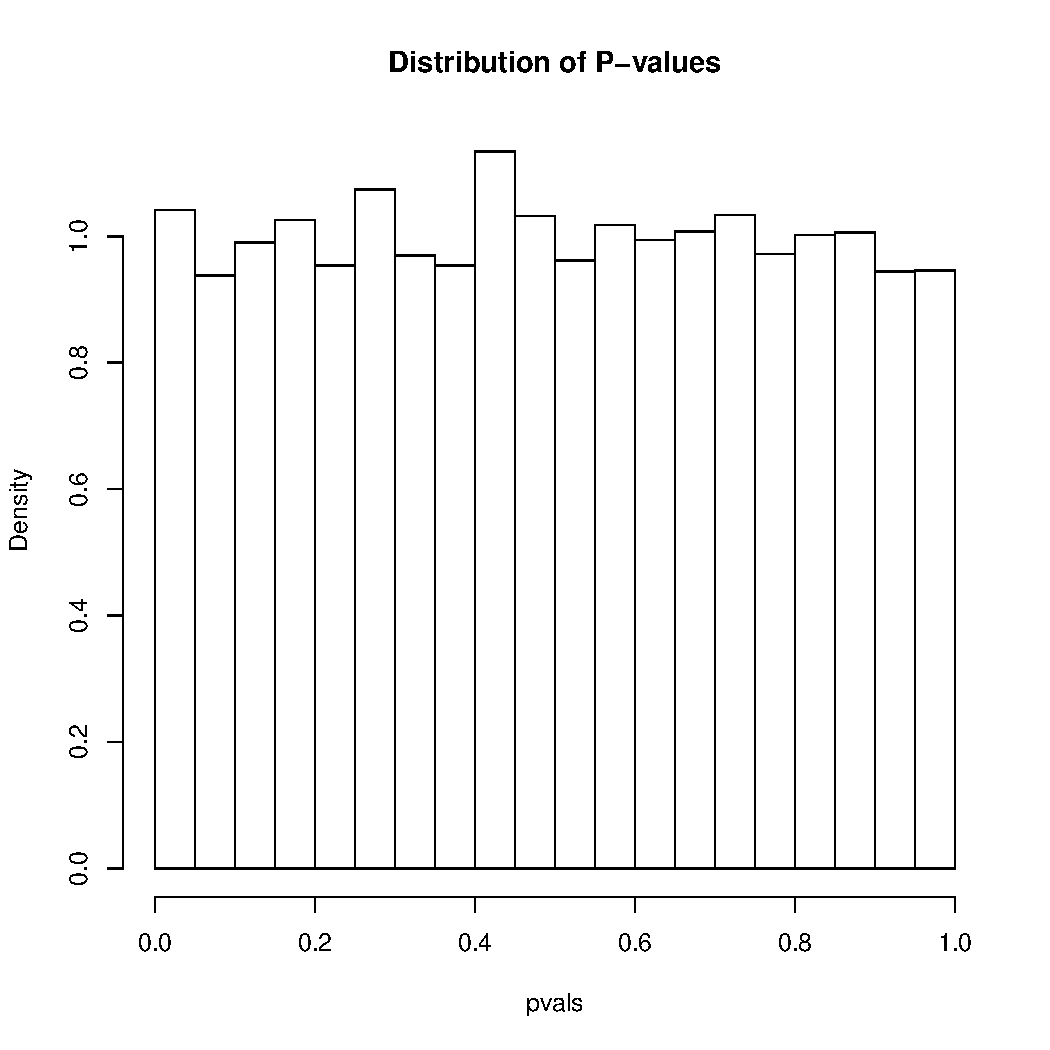
\includegraphics[width=.6\linewidth]{figure/beamer-unnamed-chunk-17-1} 

}



\end{knitrout}
  \end{itemize}
\end{frame}

\begin{frame}{Quantile-Quantile Plot}
  \begin{itemize}
  \item An important tool to assess type I error control is the
        Quantile-Quantile Plot (aka QQ-Plot)
  \item The plot should look like this under $H_0$
\begin{knitrout}\tiny
\definecolor{shadecolor}{rgb}{0.969, 0.969, 0.969}\color{fgcolor}

{\centering 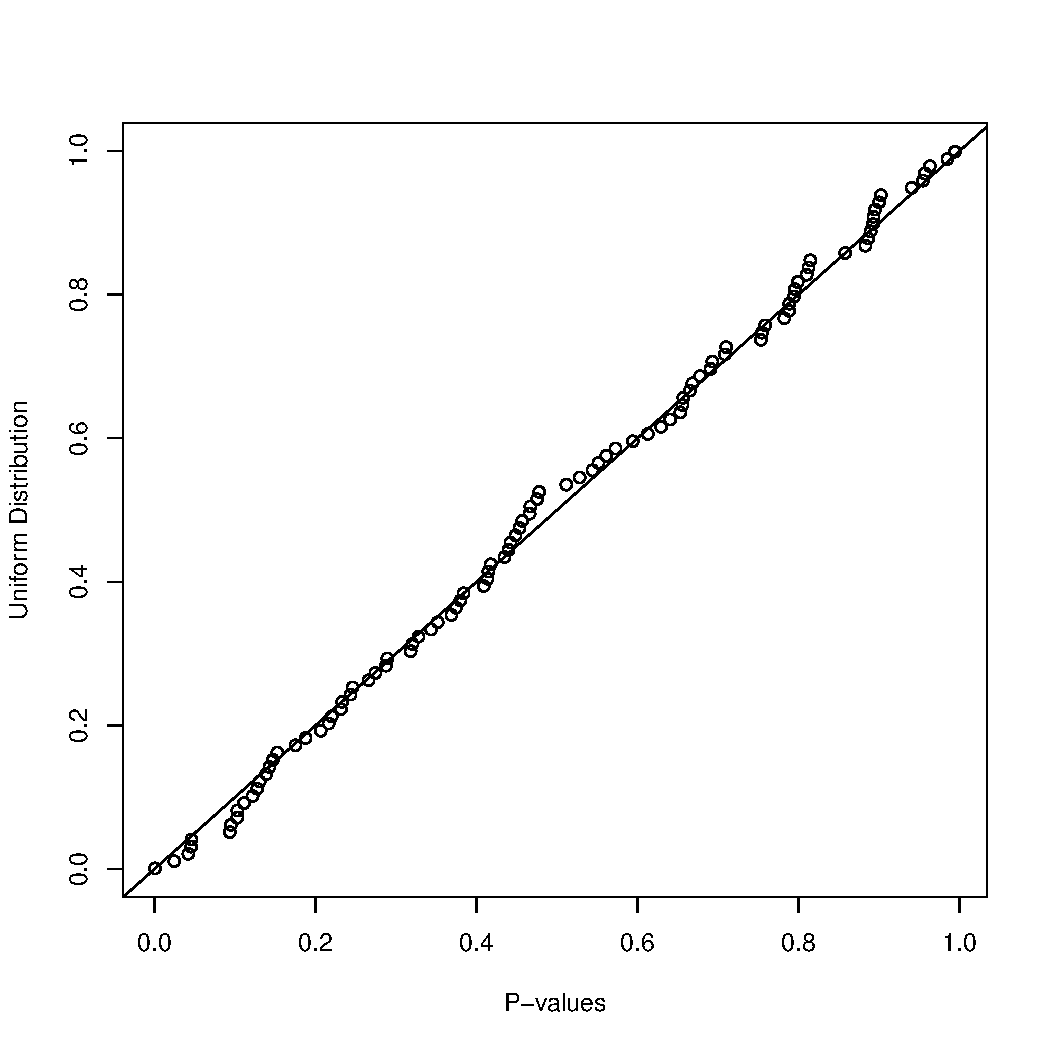
\includegraphics[width=.6\linewidth]{figure/beamer-unnamed-chunk-18-1} 

}



\end{knitrout}
  \end{itemize}
\end{frame}

\begin{frame}{Quantile-Quantile Plot: Deviation}
  \begin{itemize}
  \item A deviation in the QQ-Plot indicates that there may be evidence
        to reject $H_0$ 
  \item Or that teh decision rule is not accounting for type I error: INFLATION!!
\begin{knitrout}\tiny
\definecolor{shadecolor}{rgb}{0.969, 0.969, 0.969}\color{fgcolor}

{\centering 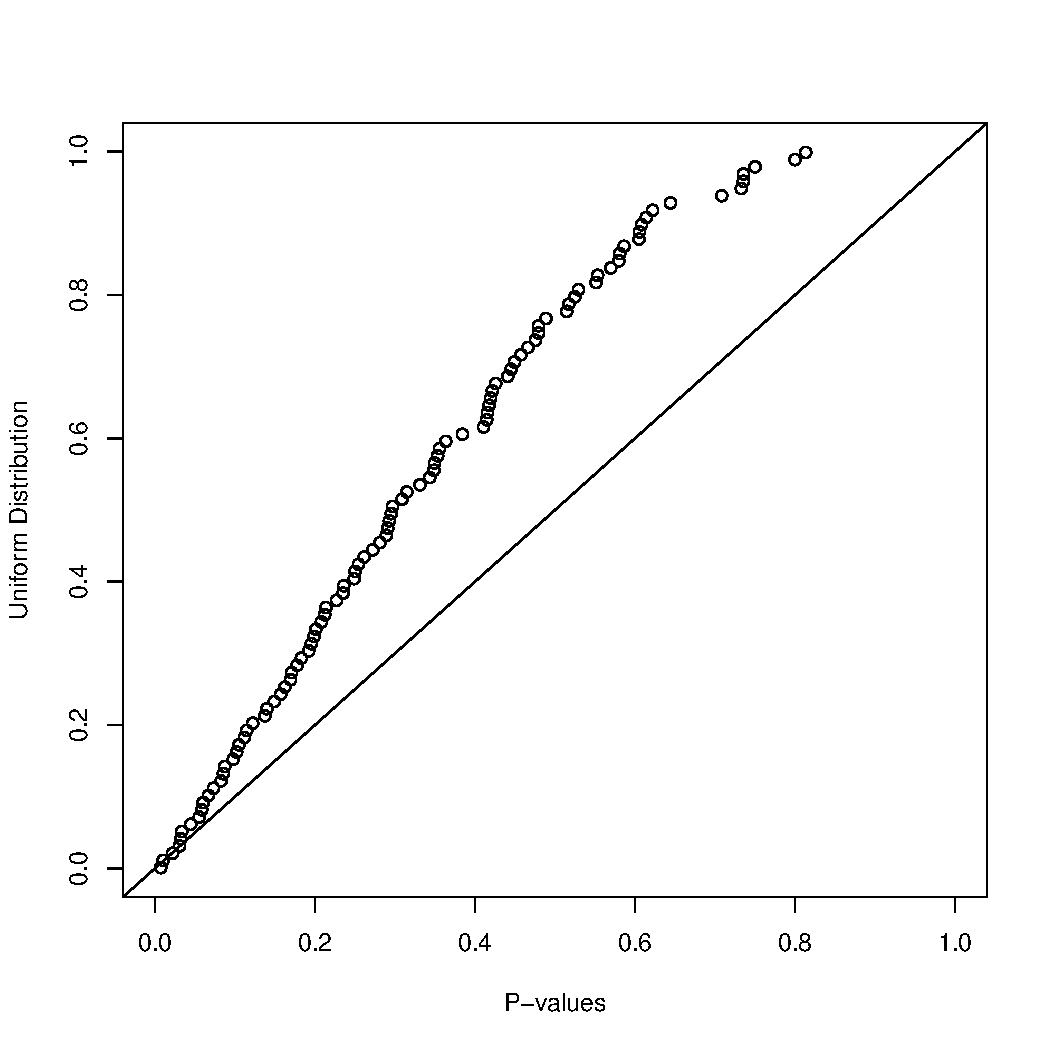
\includegraphics[width=.6\linewidth]{figure/beamer-unnamed-chunk-19-1} 

}



\end{knitrout}
  \end{itemize}
\end{frame}


\begin{frame}{Estimation}
  \begin{itemize}
  \item So far we have considered concepts and issues related to hypothesis testing
  \item What is often of interested is estimate the unknown parameters
  \item First determine how to quantify the effect size
  \item Consider the two sample problem
  \item Examples
    \begin{itemize}
    \item Mean level for the untreated group $\mu_0$
    \item Mean level for the treated group $\mu_1$
    \item Fold-change $\rho=\frac{\mu_1}{\mu_0}$
    \item Standardized difference $\Delta=|\mu_1-\mu_0|/\sigma$
  \end{itemize}
  \item Next figure out how to estimate the effect size
  \item Two types of estimates
    \begin{itemize}
    \item Point estimate
    \item Interval estimate
    \end{itemize}
  \end{itemize}
\end{frame}


\begin{frame}{Confidence Intervals}
  \begin{itemize}
  \item Example: The sample mean (the average of the observations) is a point estimate of the 
        population (true) mean
  \item It is either equal to the true value of the parameter or is not
  \item As it is a single number it does not provide any direct measure of accuracy
  \item An interval estimate incorporates some measure of accuracy
  \item Thus it is generally more appropriate to present an interval estimate
  \item A common example of an interval estimate is the confidence interval
  \end{itemize}
\end{frame}

\begin{frame}[fragile]{Estimation Example}

  \begin{itemize}  
  \item Assumption: The RNA abundance follows a normal distribution with mean $\mu=0$
        and standard deviation $\sigma=1$
  \item Goal: The population mean $\mu$ is to be estimated on the basis of sample of size
        $n=6$
  \item Objectives:
    \begin{itemize}
    \item Produce point estimate of $\mu$ 
    \item Produce a 95\% confidence interval of $\mu$
    \end{itemize}
  \item We will produce these estimates on the basis of the sample mean
  \item The sample mean is obtained by averaging the $n$ observations
  \end{itemize}
\end{frame}


\begin{frame}[fragile]{Simulate Experiment 1}
  \begin{itemize}  
  \item Simulate the data
\begin{knitrout}\tiny
\definecolor{shadecolor}{rgb}{0.969, 0.969, 0.969}\color{fgcolor}\begin{kframe}
\begin{alltt}
\hlstd{n}
\end{alltt}
\begin{verbatim}
## [1] 6
\end{verbatim}
\begin{alltt}
\hlstd{mu}
\end{alltt}
\begin{verbatim}
## [1] 0
\end{verbatim}
\begin{alltt}
\hlstd{sigma}
\end{alltt}
\begin{verbatim}
## [1] 1
\end{verbatim}
\begin{alltt}
\hlkwd{set.seed}\hlstd{(}\hlnum{12331}\hlstd{)}
\hlstd{x}\hlkwb{=}\hlkwd{rnorm}\hlstd{(n,mu,sigma)}
\end{alltt}
\end{kframe}
\end{knitrout}
\item Calculate the sample mean
\begin{knitrout}\tiny
\definecolor{shadecolor}{rgb}{0.969, 0.969, 0.969}\color{fgcolor}\begin{kframe}
\begin{alltt}
\hlkwd{mean}\hlstd{(x)}
\end{alltt}
\begin{verbatim}
## [1] -0.4014889
\end{verbatim}
\end{kframe}
\end{knitrout}
\item Calculate confidence interval
\begin{knitrout}\tiny
\definecolor{shadecolor}{rgb}{0.969, 0.969, 0.969}\color{fgcolor}\begin{kframe}
\begin{alltt}
\hlcom{# sample standard deviation}
\hlstd{s}\hlkwb{=}\hlkwd{sd}\hlstd{(x)}
\hlcom{# Margin of error}
\hlstd{error}\hlkwb{=}\hlkwd{qt}\hlstd{(}\hlnum{0.975}\hlstd{,}\hlkwc{df}\hlstd{=n}\hlopt{-}\hlnum{1}\hlstd{)}\hlopt{*}\hlstd{s}\hlopt{/}\hlkwd{sqrt}\hlstd{(n)}
\hlcom{# A 95% CI}
\hlkwd{c}\hlstd{(}\hlkwd{mean}\hlstd{(x)}\hlopt{-}\hlstd{error,}\hlkwd{mean}\hlstd{(x)}\hlopt{+}\hlstd{error)}
\end{alltt}
\begin{verbatim}
## [1] -1.4687200  0.6657421
\end{verbatim}
\end{kframe}
\end{knitrout}
 \end{itemize}
\end{frame}


\begin{frame}{Repeat the Experiment}
\begin{knitrout}\tiny
\definecolor{shadecolor}{rgb}{0.969, 0.969, 0.969}\color{fgcolor}
\begin{tabular}{r|r|r|r|r|r|r|r|r}
\hline
exp & n & mu & sigma & avg & lcl & ucl & cover & len\\
\hline
1 & 6 & 0 & 1 & 0.36 & 0.05 & 0.67 & 0 & 0.62\\
\hline
2 & 6 & 0 & 1 & 0.67 & -0.23 & 1.57 & 1 & 1.80\\
\hline
3 & 6 & 0 & 1 & -0.23 & -0.89 & 0.42 & 1 & 1.31\\
\hline
4 & 6 & 0 & 1 & -0.88 & -2.09 & 0.34 & 1 & 2.42\\
\hline
5 & 6 & 0 & 1 & -0.88 & -1.62 & -0.14 & 0 & 1.49\\
\hline
6 & 6 & 0 & 1 & 0.57 & -0.64 & 1.78 & 1 & 2.42\\
\hline
7 & 6 & 0 & 1 & -0.03 & -1.60 & 1.54 & 1 & 3.15\\
\hline
8 & 6 & 0 & 1 & -0.62 & -1.18 & -0.05 & 0 & 1.13\\
\hline
9 & 6 & 0 & 1 & -0.05 & -1.46 & 1.37 & 1 & 2.82\\
\hline
10 & 6 & 0 & 1 & 0.21 & -0.92 & 1.34 & 1 & 2.25\\
\hline
\end{tabular}


\end{knitrout}
\end{frame}
\begin{frame}{Confidence Interval: Common Misunderstanding}
  \begin{itemize}
  \item A (not the) 95\% CI for the mean based on the first experiment was
        $(0.05,0.67)$
  \item A (not the) 95\% CI for the mean based on the second experiment was
        $(\ensuremath{-0.23},1.57)$
  \item It is wrong to say that the probability that the first CI does not contain the true value
        $\mu=0$ is 95\%
  \item It is also wrong to say that the probability that the second CI contains the true value
        $\mu=0$ is 95\%
  \item We conduct one and only was experiment
  \item Based on the first experiment, we can say that we are 95\% confident that it contains the true value
  \item That is of course not the case
  \item If we repeated the experiment a large number of times, 95\% of the CIs would cover the true
    value
  \item We are 95\% confident that the first experiment is among these (which it is not)
  \end{itemize}
\end{frame}


\begin{frame}{Repeat the Experiment}

  
  \begin{itemize}
  \item Now repeat experiment with a sample size of
    $n=12$.
\begin{knitrout}\tiny
\definecolor{shadecolor}{rgb}{0.969, 0.969, 0.969}\color{fgcolor}
\begin{tabular}{r|r|r|r|r|r|r|r|r}
\hline
exp & n & mu & sigma & avg & lcl & ucl & cover & len\\
\hline
1 & 12 & 0 & 1 & 0.07 & -0.50 & 0.65 & 1 & 1.16\\
\hline
2 & 12 & 0 & 1 & -0.07 & -0.66 & 0.51 & 1 & 1.16\\
\hline
3 & 12 & 0 & 1 & 0.68 & 0.11 & 1.25 & 0 & 1.14\\
\hline
4 & 12 & 0 & 1 & -0.32 & -1.12 & 0.49 & 1 & 1.60\\
\hline
5 & 12 & 0 & 1 & -0.14 & -0.82 & 0.55 & 1 & 1.37\\
\hline
6 & 12 & 0 & 1 & -0.26 & -0.81 & 0.30 & 1 & 1.11\\
\hline
7 & 12 & 0 & 1 & -0.13 & -0.47 & 0.21 & 1 & 0.68\\
\hline
8 & 12 & 0 & 1 & -0.20 & -0.76 & 0.35 & 1 & 1.10\\
\hline
9 & 12 & 0 & 1 & 0.19 & -0.32 & 0.70 & 1 & 1.02\\
\hline
10 & 12 & 0 & 1 & -0.46 & -1.13 & 0.21 & 1 & 1.34\\
\hline
\end{tabular}


\end{knitrout}
\item Compare the widths of the CIs
\end{itemize}

\end{frame}


\begin{frame}{Quick Note: Estimate versus Estimator}
  \begin{itemize}
  \item We use the terms estimate and estimators interchangeably
  \item There is a subtle but important distinction
  \item Suppose that you decide to estimate the population mean using the sample mean (once you get the data)
  \item The sample mean is the estimator
  \item Its outcome is random before you collect the data
  \item Once you collect the data and plug them into the estimator you get an (not the) estimate
  \end{itemize}
\end{frame}
\section[Model]{Model Building Illustration}


\begin{frame}{Intra- and Inter-subject Variability}
  \begin{itemize}
    \item In most experiments, including RNA-Seq, the variability may not be exclusively due to measurement
      error
  \item Another source could be due to repeated measurements
  \item or sampling from strains or cell lines
  \item or due to batch effects
  \item We will motivate these ideas using a classical toy example
  \item We will illustrate the caveats of properly
        accounting for these two sources of variability through
        two simulation studies
  \end{itemize}
\end{frame}


\begin{frame}[fragile]{Rails Data}
  \begin{itemize}
  \item Observation adjusted travel time for ultrasonic head-waves in the rail 
        (nanoseconds).
  \item Data set: 6 rails; the travel time is sampled three times per
        rail
  \item Eighteen measurements
  \item Six Experimental Units
  \item Implicit assumption: The six rails are randomly selected
        from a {\it large} pool of rails
  \item What is of interest is neither the batch or any of these
        6 rails (specifically)
  \item What is of interest is the population (the huge pool)
  \end{itemize}
\end{frame}

\begin{frame}{Rail Data}
\begin{knitrout}\tiny
\definecolor{shadecolor}{rgb}{0.969, 0.969, 0.969}\color{fgcolor}

{\centering 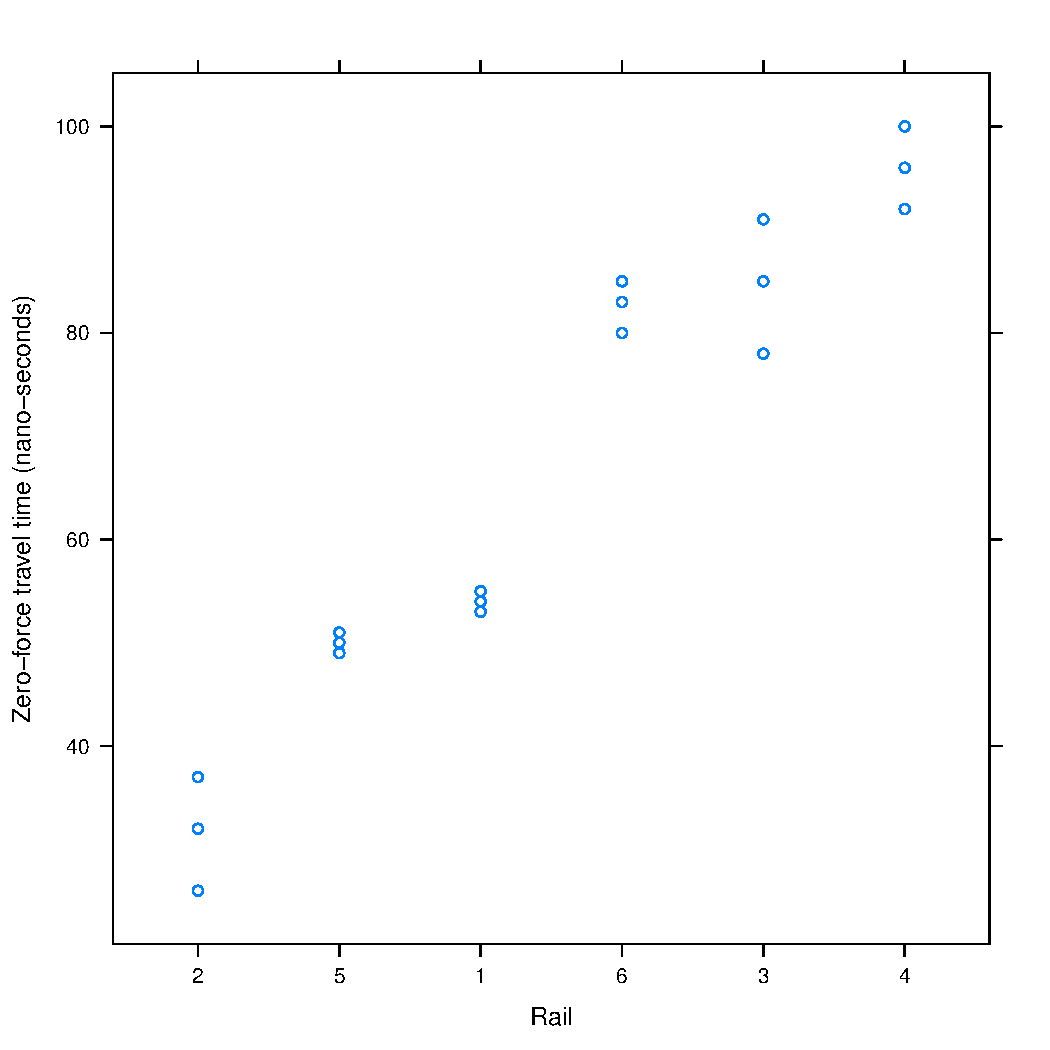
\includegraphics[width=.6\linewidth]{figure/beamer-railplots-1} 

}



\end{knitrout}

\end{frame}

\begin{frame}{Rail Data: Model Formulation}
  \begin{itemize}
  \item $\mu$ denotes the {\it true} travel time
  \item $\mu$ is an unknown fixed quantity
  \item $Y_i$ denotes the {\it observed} travel time 
        (for observation $i=1,\ldots,18$)
  \item In absence of noise, true value $\mu$
        is observed
  \item In other words, $Y_{i}=\mu$ for $i=1,\ldots,18$
  \end{itemize}
\end{frame}


\begin{frame}{Important Fact about Normal Distribution}
  \begin{itemize}
  \item Consider a normal distribution with mean 0 and standard deviation
        $\sigma$
  \item If the data are shifted by a constant $\mu$, then
    \begin{enumerate}
    \item  resulting
        distribution remains normal
     \item The mean of the new distribution is $\mu+0=\mu$
  \item Its standard deviation remains unchanged
    \end{enumerate}
  \item The last two (but not first) property are true for any distribution
  \end{itemize}
\end{frame}

\begin{frame}{Shift Normal Distribution}
\begin{knitrout}\tiny
\definecolor{shadecolor}{rgb}{0.969, 0.969, 0.969}\color{fgcolor}

{\centering 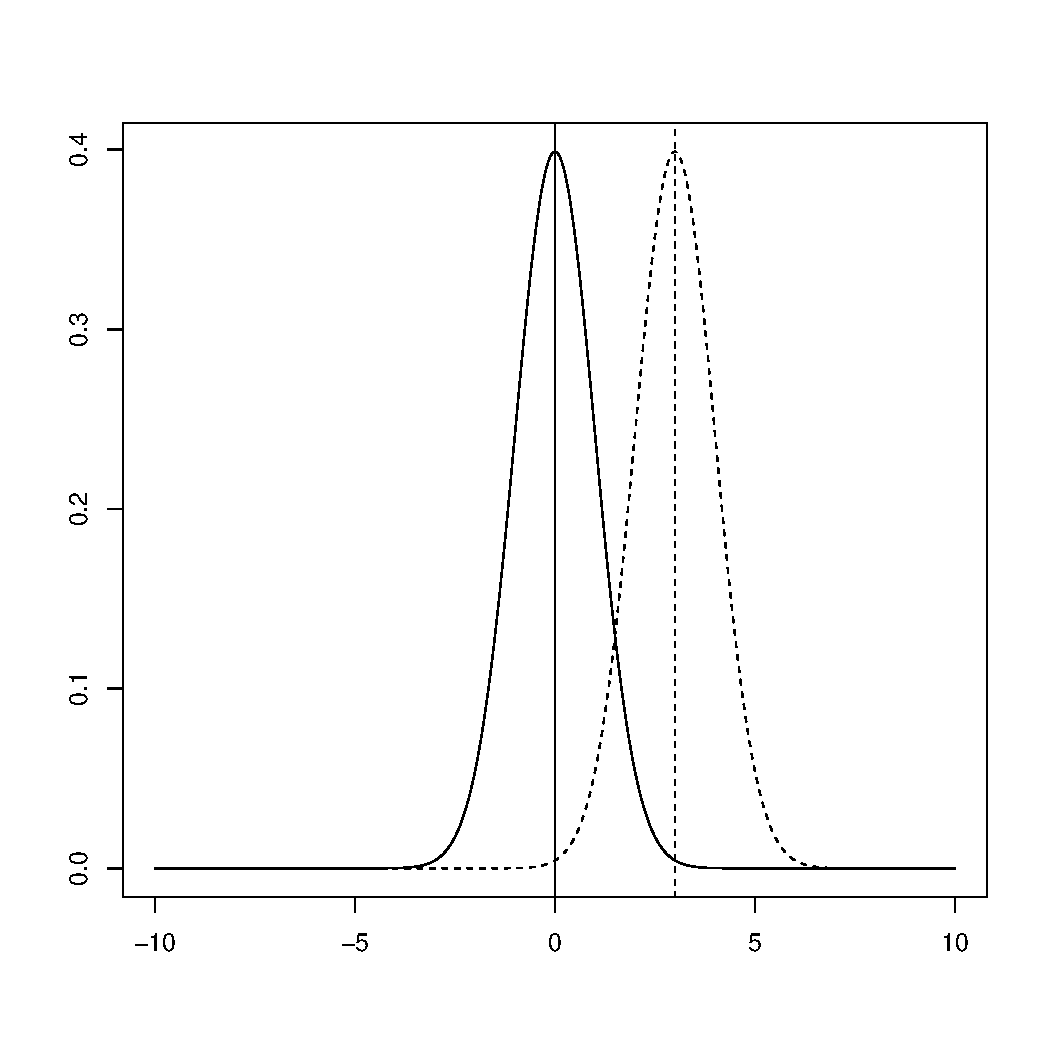
\includegraphics[width=.6\linewidth]{figure/beamer-unnamed-chunk-27-1} 

}



\end{knitrout}
\end{frame}


\begin{frame}{Rail Data: Simple Model}
  \begin{itemize}
  \item What is observed is a distorted version of $\mu$
    \begin{equation*}
      Y_{i}=\mu+\epsilon_i
    \end{equation*}
    \item Notes:
    \begin{itemize}
    \item  $Y_i$ is observable
    \item  $\epsilon_i$ is {\it not} observable
    \item $\mu$ is an unknown parameter
    \end{itemize}
 \item The variability observed here is exclusively attributed to the measurement error
      $\epsilon_i$
  \end{itemize}
\end{frame}

\begin{frame}[fragile]{Linear Model}
\begin{knitrout}\tiny
\definecolor{shadecolor}{rgb}{0.969, 0.969, 0.969}\color{fgcolor}\begin{kframe}
\begin{alltt}
\hlkwd{summary}\hlstd{(}\hlkwd{lm}\hlstd{(travel}\hlopt{~}\hlnum{1}\hlstd{,}\hlkwc{data}\hlstd{=Rail))}
\end{alltt}
\begin{verbatim}
## 
## Call:
## lm(formula = travel ~ 1, data = Rail)
## 
## Residuals:
##    Min     1Q Median     3Q    Max 
## -40.50 -16.25   0.00  18.50  33.50 
## 
## Coefficients:
##             Estimate Std. Error t value Pr(>|t|)    
## (Intercept)   66.500      5.573   11.93  1.1e-09 ***
## ---
## Signif. codes:  0 '***' 0.001 '**' 0.01 '*' 0.05 '.' 0.1 ' ' 1
## 
## Residual standard error: 23.65 on 17 degrees of freedom
\end{verbatim}
\end{kframe}
\end{knitrout}
\end{frame}

\begin{frame}{Rail Data: Account for Two Source of Variability}
  \begin{itemize}
  \item What is observed is a distorted version of $\mu$
  \item It is distorted by a ra
  \item $Y_{ij}$: Index the rail by $i=1,\ldots,6$ and the replicate by $j=1,2,3$
  \item $Y_{23}$: The obeservation for the third replicate for rail 2
   \item Model
    \begin{equation*}
      Y_{ij}=\mu+b_i+\epsilon_{ij}
    \end{equation*}
    \item Notes:
    \begin{itemize}
    \item  $Y_{ij}$ is observable
    \item $b_i$ is {\it not} observable
    \item  $\epsilon_{ij}$ is {\it not} observable
    \item $\mu$ is an unknown parameter
    \end{itemize}
  \end{itemize}
\end{frame}

\begin{frame}[fragile]{Linear Mixed Effects Model}
\begin{knitrout}\tiny
\definecolor{shadecolor}{rgb}{0.969, 0.969, 0.969}\color{fgcolor}\begin{kframe}
\begin{alltt}
\hlkwd{lme}\hlstd{(travel}\hlopt{~}\hlnum{1}\hlstd{,}\hlkwc{random}\hlstd{=}\hlopt{~}\hlnum{1}\hlopt{|}\hlstd{Rail,}\hlkwc{data}\hlstd{=Rail)}
\end{alltt}
\begin{verbatim}
## Linear mixed-effects model fit by REML
##   Data: Rail 
##   Log-restricted-likelihood: -61.0885
##   Fixed: travel ~ 1 
## (Intercept) 
##        66.5 
## 
## Random effects:
##  Formula: ~1 | Rail
##         (Intercept) Residual
## StdDev:    24.80547 4.020779
## 
## Number of Observations: 18
## Number of Groups: 6
\end{verbatim}
\end{kframe}
\end{knitrout}
\end{frame}


\begin{frame}[fragile]{Is the Mixed Model Adequate?}
  \begin{itemize}
  \item Assumptions:
    \begin{itemize}
    \item $b_i$ is normally distributed $N[0,\sigma^2_b]$
    \item $\sigma^2_b$ does {\it not} depend on $i$ (homoscedastic) 
    \item $\epsilon_{ij}$ is normally distributed $N[0,\sigma^2_e]$
    \item $\sigma^2_e$ does {\it not} depend on $i$ or $j$ (homoscedastic)
    \item Error model is additive (could be multiplicative)
    \end{itemize}
  \end{itemize}
\end{frame}


\begin{frame}[fragile]{Example 1: Setup}
  \begin{itemize}
  \item What are the ramifications for ignoring the clustering?
  \item We will sample 6 experimental units each with three replicates
  \item $\mu=0, \sigma_e=0.25,\sigma_b=0.5$
  \end{itemize}
  
\begin{knitrout}\tiny
\definecolor{shadecolor}{rgb}{0.969, 0.969, 0.969}\color{fgcolor}

{\centering 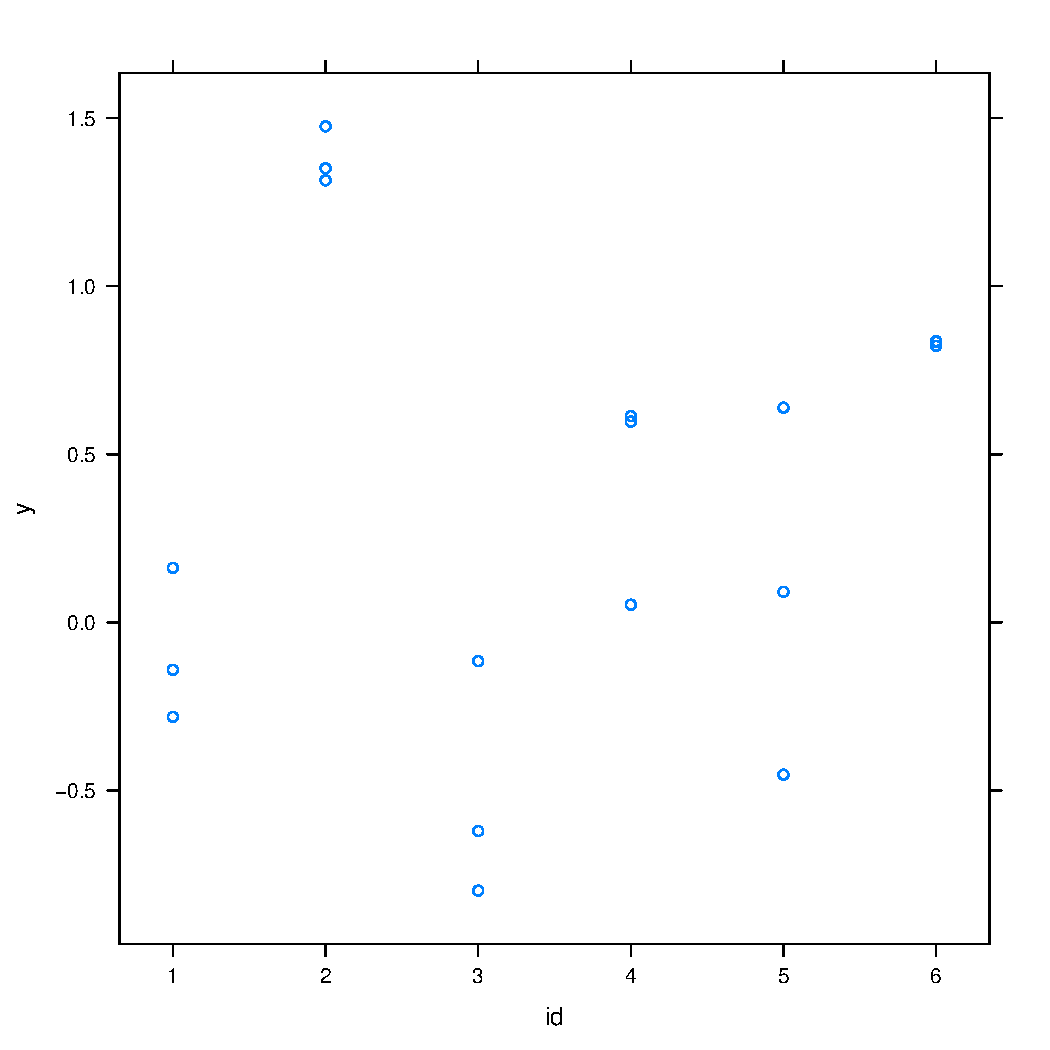
\includegraphics[width=.6\linewidth]{figure/beamer-unnamed-chunk-30-1} 

}



\end{knitrout}
\end{frame}


\begin{frame}[fragile]{Example 1: Simulation}

  
   \begin{itemize}
  \item Simulation outline
  \begin{enumerate}
  \item Simulate a data set
  \item Test $H_0: \mu=0$ ignoring the random effect (save {\it P}-value) 
  \item Test $H_0: \mu=0$ accounting for the random effect (save {\it P}-value) 
  \end{enumerate}
  \item Repeat the three steps 999 additional times
  \item Given that the {\it true} $\mu=0$ (by design), we would expect
        50 of these  {\it P}-values to be less than 0.05
  \item Why?
    \end{itemize}
\end{frame}

\begin{frame}[fragile]{Example 1: Results}
\begin{knitrout}\tiny
\definecolor{shadecolor}{rgb}{0.969, 0.969, 0.969}\color{fgcolor}\begin{kframe}
\begin{alltt}
\hlkwd{set.seed}\hlstd{(}\hlnum{210}\hlstd{)}
\hlstd{res}\hlkwb{=}\hlkwd{replicate}\hlstd{(B3,}\hlkwd{sim.ranef}\hlstd{(}\hlnum{3}\hlstd{,}\hlnum{6}\hlstd{,}\hlnum{0.25}\hlstd{,}\hlnum{0.5}\hlstd{,}\hlkwc{verbose}\hlstd{=}\hlnum{FALSE}\hlstd{))}
\hlkwd{mean}\hlstd{(res[}\hlnum{1}\hlstd{,]}\hlopt{<}\hlnum{0.05}\hlstd{)}
\end{alltt}
\begin{verbatim}
## [1] 0.247
\end{verbatim}
\begin{alltt}
\hlkwd{mean}\hlstd{(res[}\hlnum{2}\hlstd{,]}\hlopt{<}\hlnum{0.05}\hlstd{)}
\end{alltt}
\begin{verbatim}
## [1] 0.072
\end{verbatim}
\end{kframe}
\end{knitrout}
\begin{itemize}
\item The empirical type I error rate when not accounting for the random
      effect is 0.25.
\item This inflated by a factor of 4.9.
\item The empirical error rate when accounting for the random effect
  is slightly inflated
\item This is due to the small sample size ($n=6$)
\item More on this later.
\end{itemize}
\end{frame}


\begin{frame}[fragile]{Example 1: Results}
\begin{knitrout}\tiny
\definecolor{shadecolor}{rgb}{0.969, 0.969, 0.969}\color{fgcolor}

{\centering 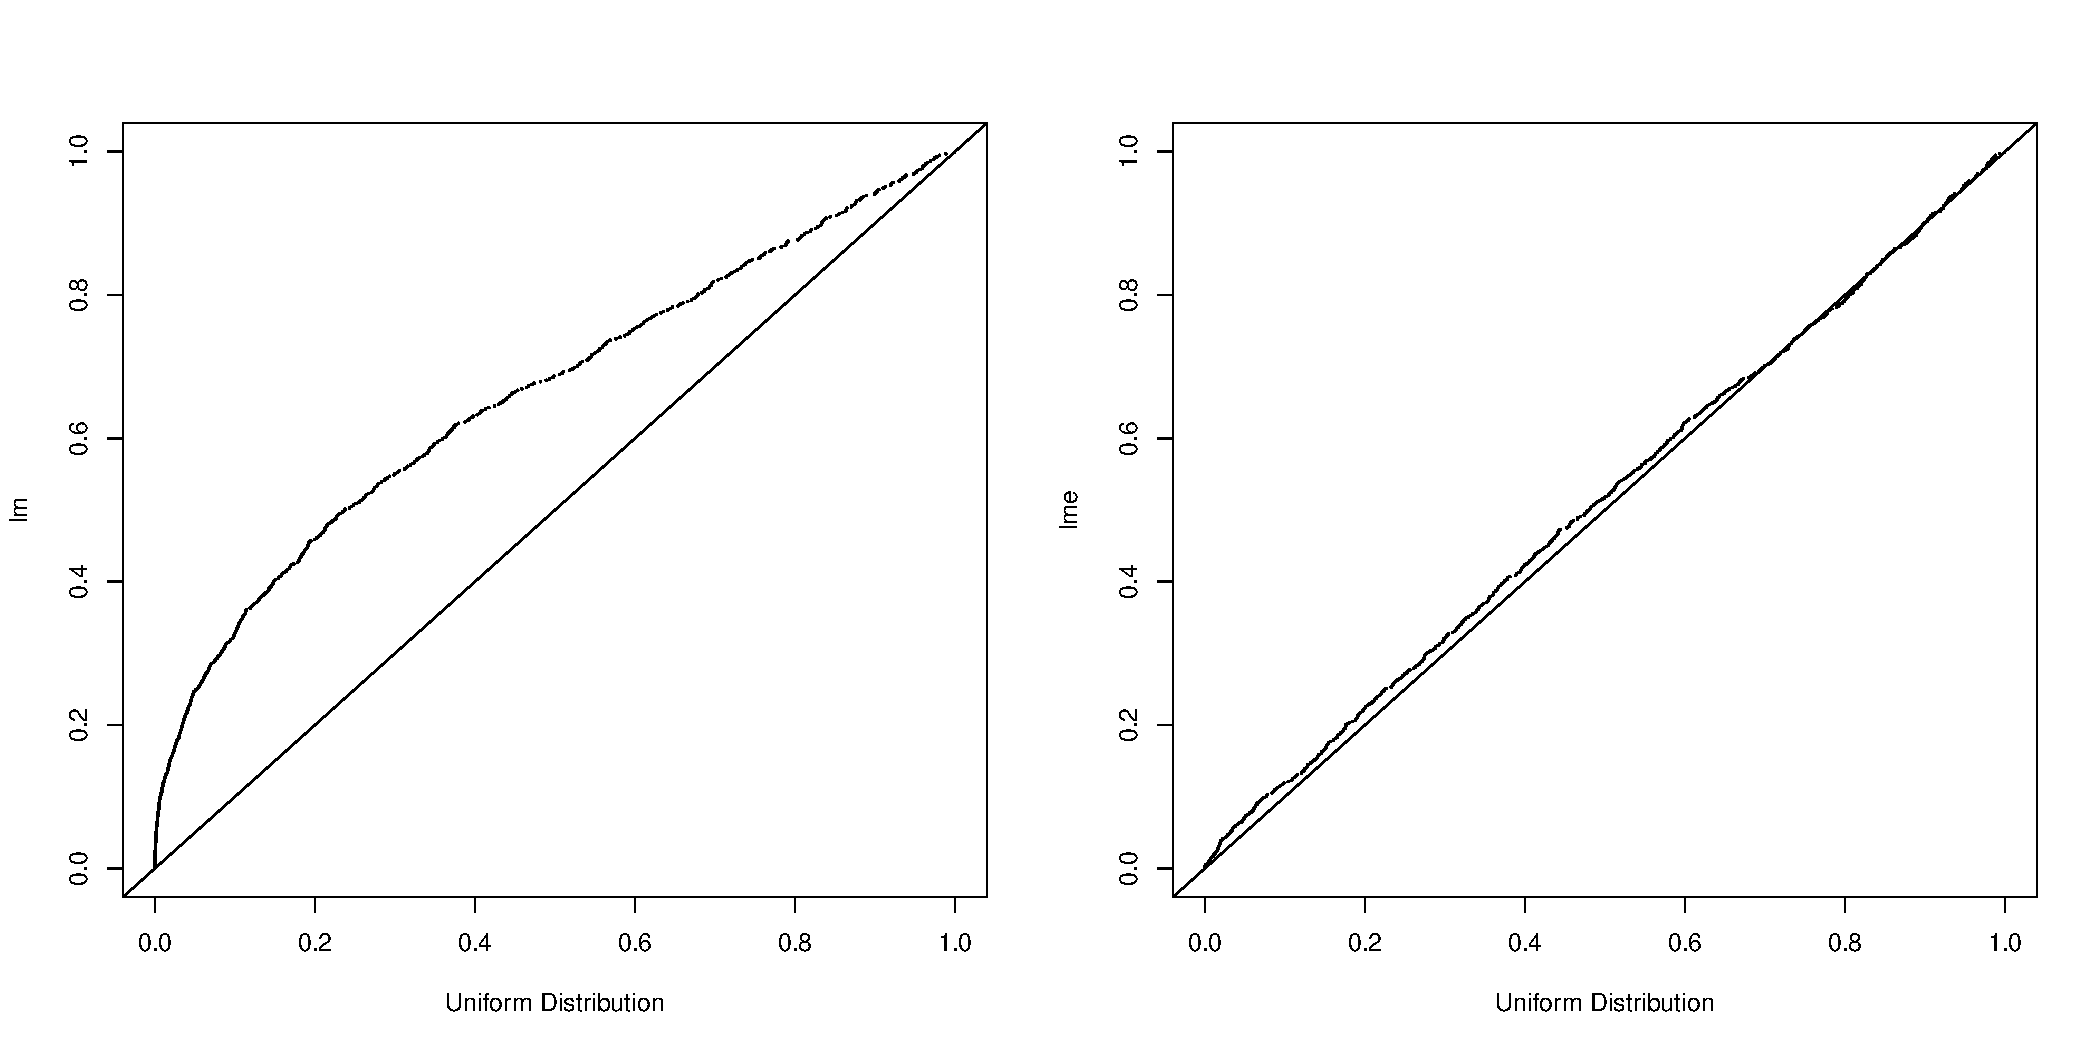
\includegraphics[width=1.1\linewidth]{figure/beamer-unnamed-chunk-33-1} 

}



\end{knitrout}
\end{frame}

\begin{frame}[fragile]{Example 1: Results}
\begin{knitrout}\tiny
\definecolor{shadecolor}{rgb}{0.969, 0.969, 0.969}\color{fgcolor}

{\centering 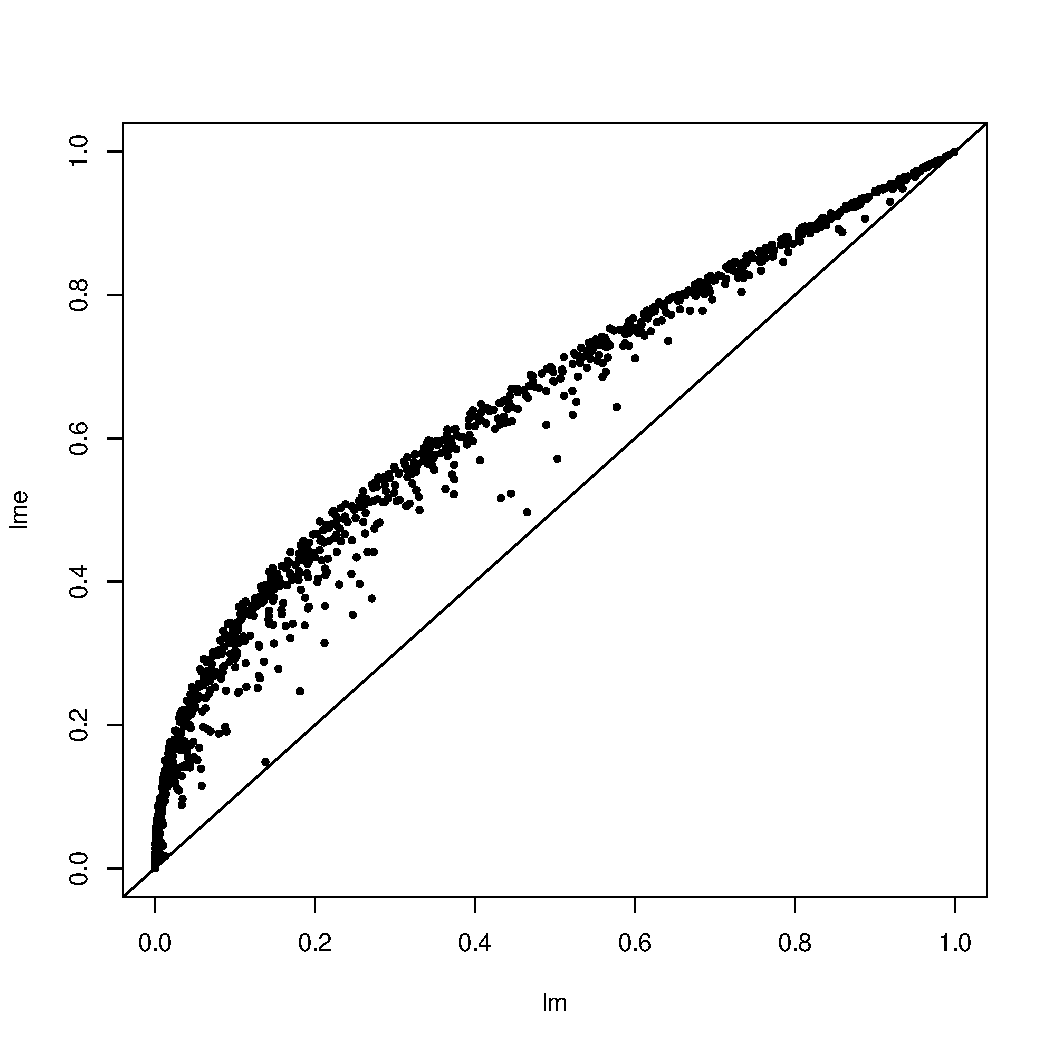
\includegraphics[width=.6\linewidth]{figure/beamer-unnamed-chunk-34-1} 

}



\end{knitrout}
\end{frame}

\begin{frame}[fragile]{Example 1: Results}
  \begin{itemize}
  \item Now, we repeat the simulation with a larger sample size
  \end{itemize}
\begin{knitrout}\tiny
\definecolor{shadecolor}{rgb}{0.969, 0.969, 0.969}\color{fgcolor}\begin{kframe}
\begin{alltt}
\hlstd{res}\hlkwb{=}\hlkwd{replicate}\hlstd{(B3,}\hlkwd{sim.ranef}\hlstd{(}\hlnum{3}\hlstd{,}\hlnum{50}\hlstd{,}\hlnum{0.25}\hlstd{,}\hlnum{0.5}\hlstd{,}\hlkwc{verbose}\hlstd{=}\hlnum{FALSE}\hlstd{))}
\hlkwd{mean}\hlstd{(res[}\hlnum{1}\hlstd{,]}\hlopt{<}\hlnum{0.05}\hlstd{)}
\end{alltt}
\begin{verbatim}
## [1] 0.215
\end{verbatim}
\begin{alltt}
\hlkwd{mean}\hlstd{(res[}\hlnum{2}\hlstd{,]}\hlopt{<}\hlnum{0.05}\hlstd{)}
\end{alltt}
\begin{verbatim}
## [1] 0.052
\end{verbatim}
\end{kframe}
\end{knitrout}
\begin{itemize}
\item The empirical type I error when not accounting for the random effect
      remains inflated by a factor of  4.3.
      \item The empirical type I error  when accounting for the random effect is now right about the nominal level of 0.05
\end{itemize}
 
\end{frame}

\begin{frame}{Example 2: Setup}
  \begin{itemize}
  \item Now consider the two-sample problem we have previously considered
        with a twist
  \item Question: Does treatment alter the distribution of the RNA level of a given gene?
  \item Assumptions:
    \begin{itemize}
    \item the RNA level for the untreated group follows a normal distribution with mean $\mu_0$ and
        variance $\sigma^2$
     \item The RNA level for the treated group follows a normal distribution with mean $\mu_1$ and
        variance $\sigma^2$
    \end{itemize}
 \item Sample $n$ units from each treatments in replicates of 3
 \item Apply the two-sample t-test which does not account for the clustering
  \end{itemize}
\end{frame}



\begin{frame}[fragile]{Example 2: Simulation}


\begin{knitrout}\tiny
\definecolor{shadecolor}{rgb}{0.969, 0.969, 0.969}\color{fgcolor}\begin{kframe}
\begin{alltt}
\hlkwd{set.seed}\hlstd{(}\hlnum{2314}\hlstd{)}
\hlcom{# Simulate with no clustering effect (sb=0)}
\hlstd{pval0}\hlkwb{=}\hlkwd{replicate}\hlstd{(B3,}\hlkwd{sim.twosample.clustered}\hlstd{(}\hlnum{3}\hlstd{,}\hlnum{10}\hlstd{,}\hlnum{0.25}\hlstd{,}\hlnum{0}\hlstd{))}
\hlcom{# Simulate with no clustering effect (sb>0)}
\hlstd{pval1}\hlkwb{=}\hlkwd{replicate}\hlstd{(B3,}\hlkwd{sim.twosample.clustered}\hlstd{(}\hlnum{3}\hlstd{,}\hlnum{10}\hlstd{,}\hlnum{0.25}\hlstd{,}\hlnum{0.5}\hlstd{))}
\hlkwd{mean}\hlstd{(pval0}\hlopt{<}\hlnum{0.05}\hlstd{)}
\end{alltt}
\begin{verbatim}
## [1] 0.049
\end{verbatim}
\begin{alltt}
\hlkwd{mean}\hlstd{(pval1}\hlopt{<}\hlnum{0.05}\hlstd{)}
\end{alltt}
\begin{verbatim}
## [1] 0.252
\end{verbatim}
\end{kframe}
\end{knitrout}
\begin{itemize}
\item The empirical type I error when there is no clustering
      effect is 0.049
\item The empirical type I error when there is a clustering effect is
      0.25
\item This off by a factor of 5!
\end{itemize}
\end{frame}



\section[Classification]{Elements of Supervised Learning}





\begin{frame}
  \frametitle{Classification Problem}
\begin{knitrout}\tiny
\definecolor{shadecolor}{rgb}{0.969, 0.969, 0.969}\color{fgcolor}

{\centering 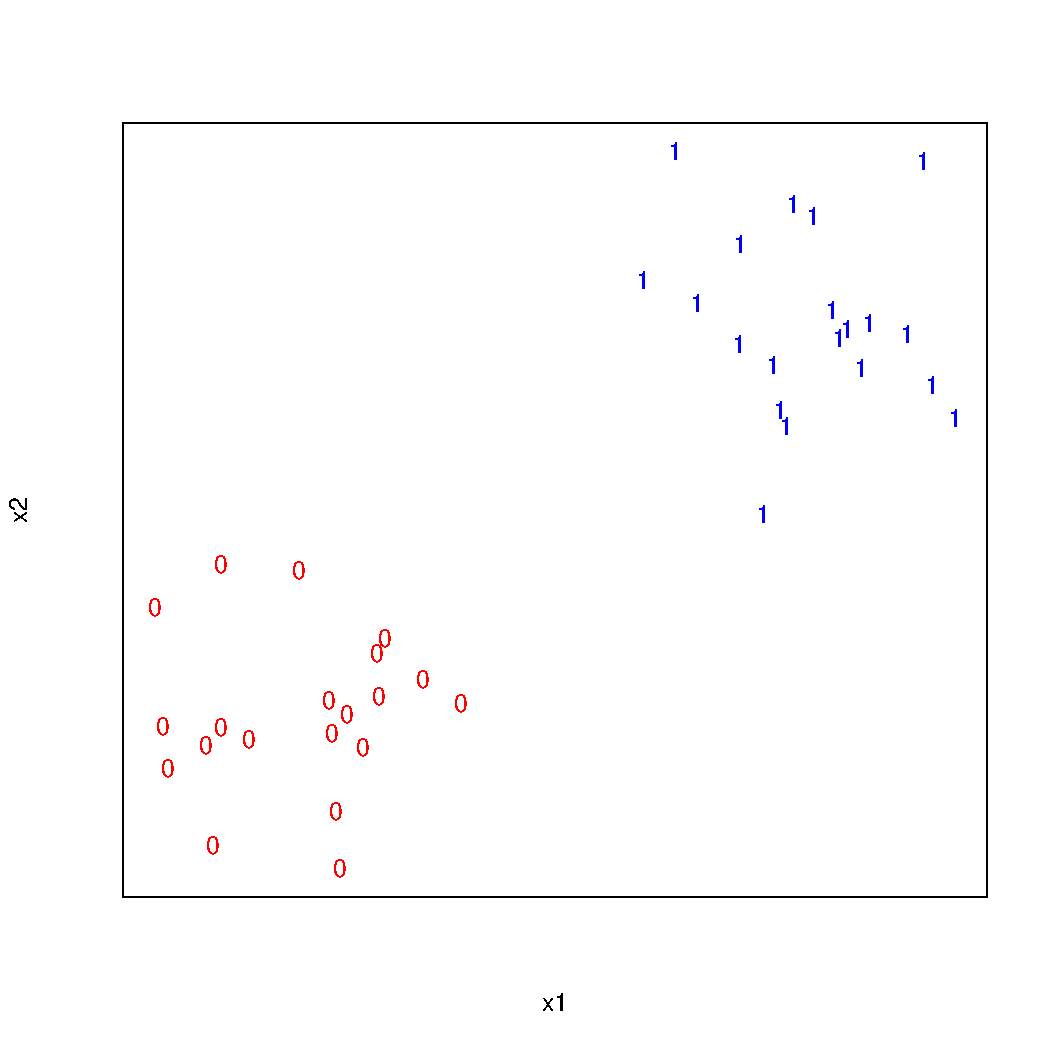
\includegraphics[width=.6\linewidth]{figure/beamer-predmod1-1} 

}



\end{knitrout}
\end{frame}

\begin{frame}
  \frametitle{Clear-cut case}
\begin{knitrout}\tiny
\definecolor{shadecolor}{rgb}{0.969, 0.969, 0.969}\color{fgcolor}

{\centering 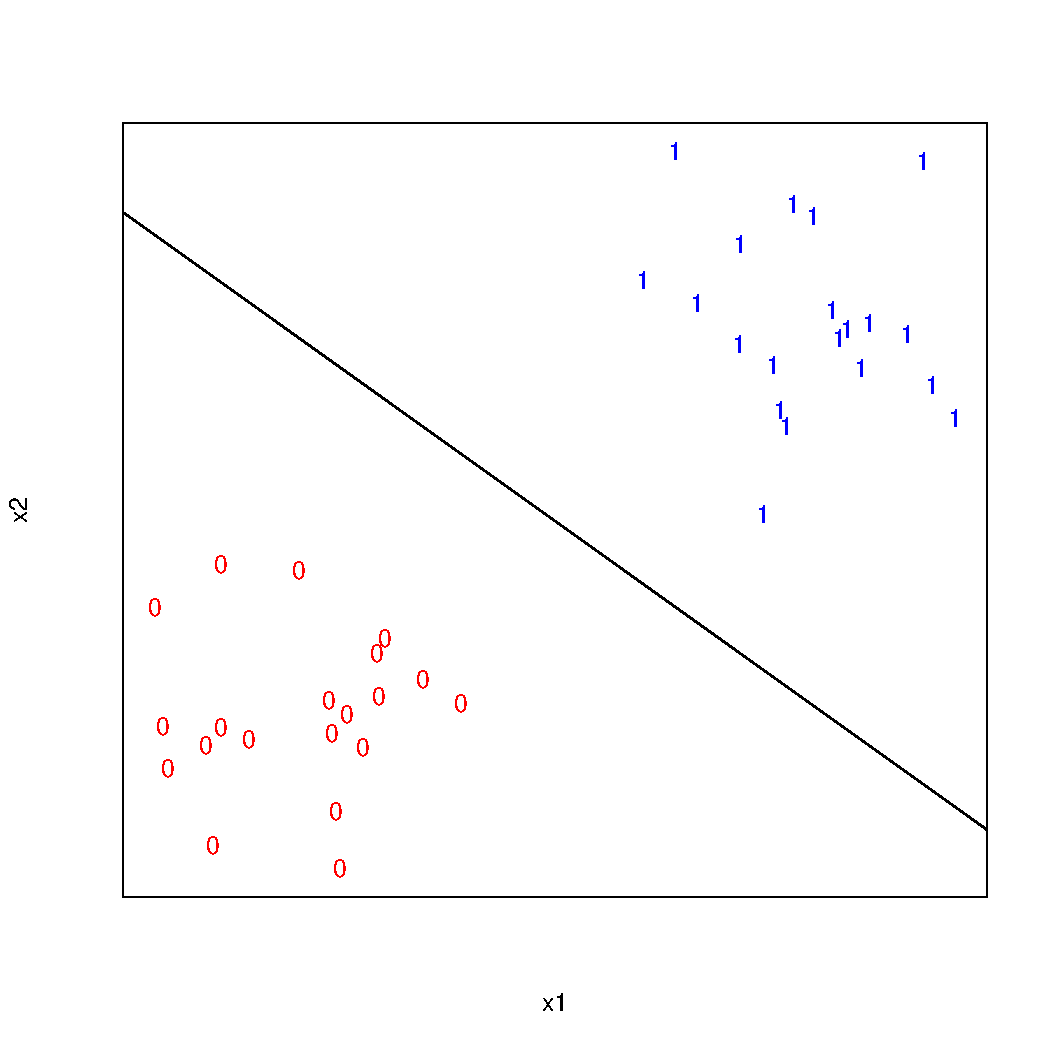
\includegraphics[width=.6\linewidth]{figure/beamer-predmod2-1} 

}



\end{knitrout}
\end{frame}

\begin{frame}
  \frametitle{Clear-cut case?}
\begin{knitrout}\tiny
\definecolor{shadecolor}{rgb}{0.969, 0.969, 0.969}\color{fgcolor}

{\centering 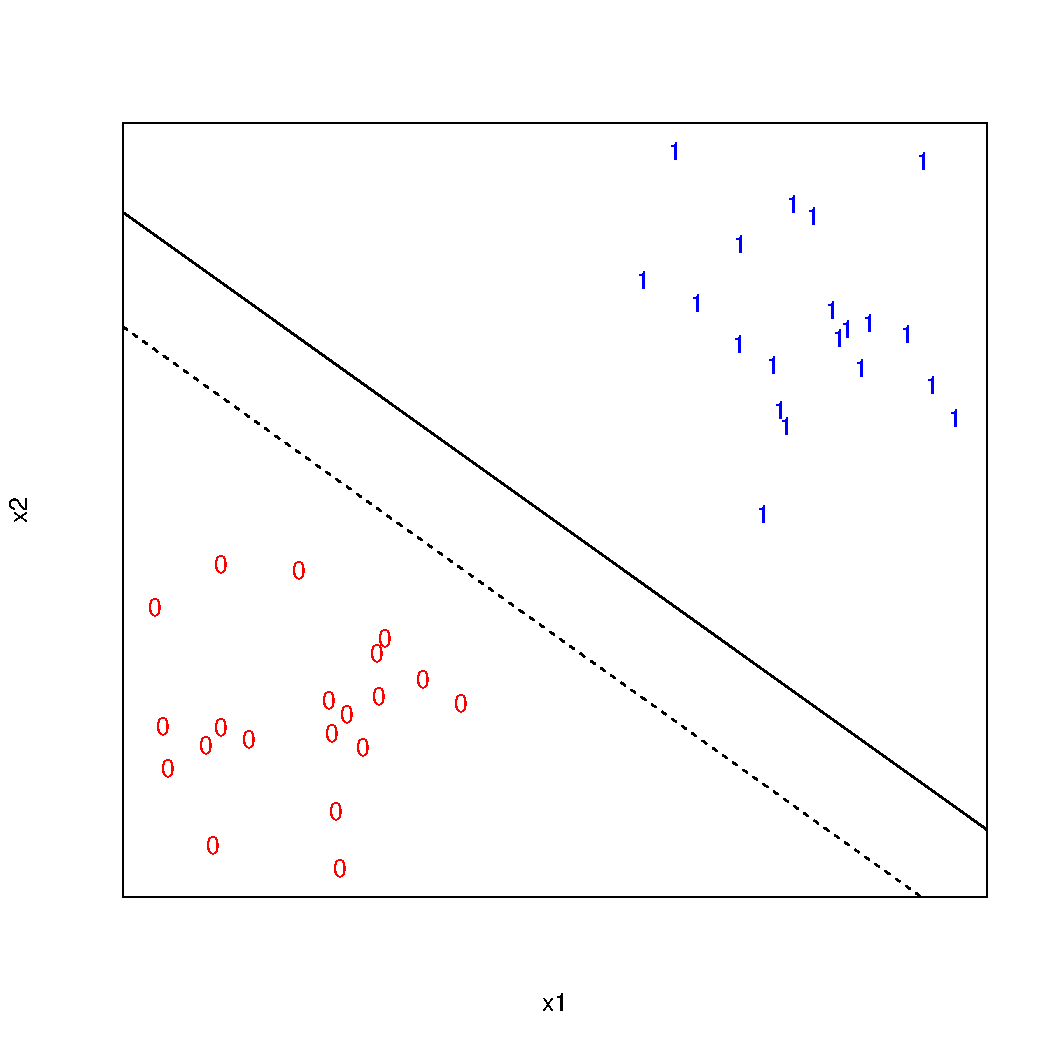
\includegraphics[width=.6\linewidth]{figure/beamer-predmod3-1} 

}



\end{knitrout}
\end{frame}

\begin{frame}
  \frametitle{Clear-cut case??}
\begin{knitrout}\tiny
\definecolor{shadecolor}{rgb}{0.969, 0.969, 0.969}\color{fgcolor}

{\centering 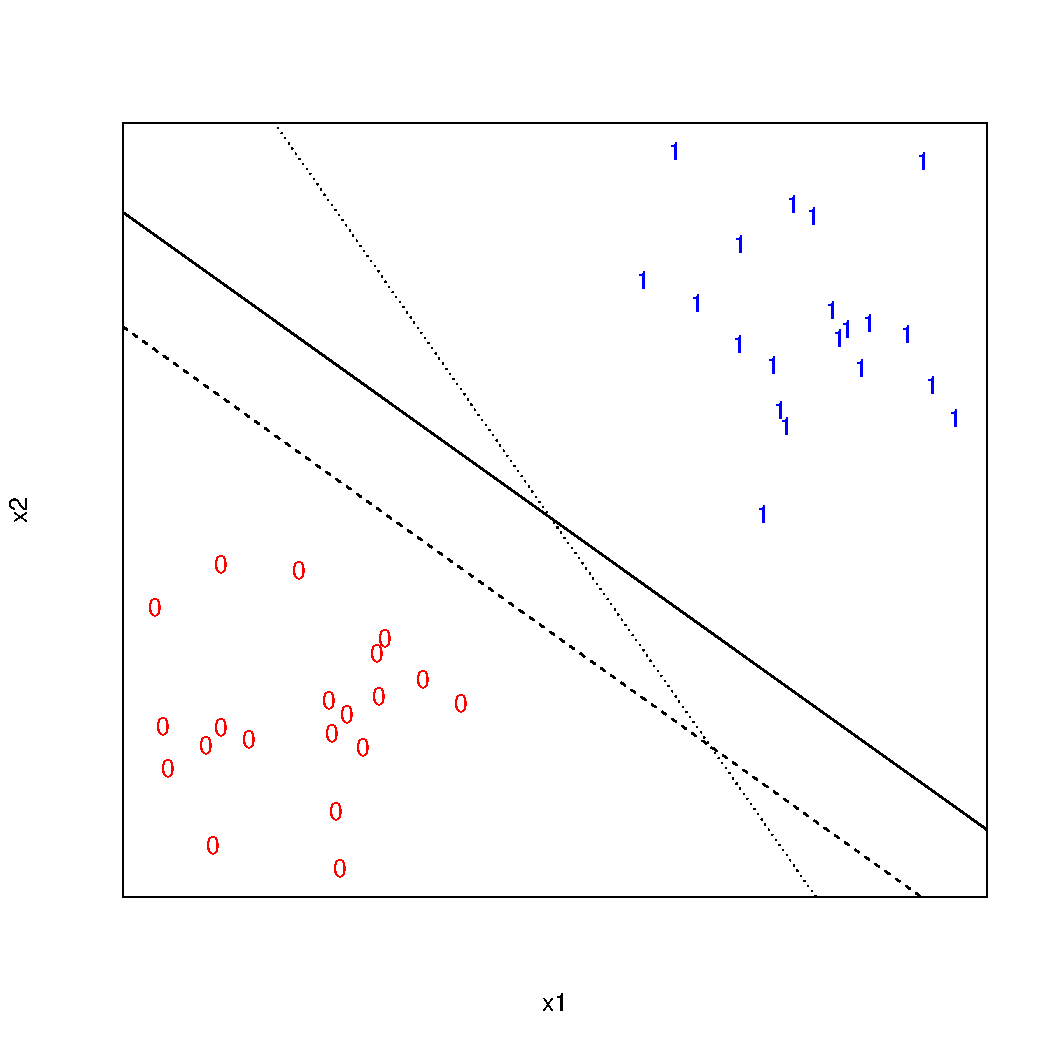
\includegraphics[width=.6\linewidth]{figure/beamer-predmod3a-1} 

}



\end{knitrout}
\end{frame}








\begin{frame}
  \frametitle{Less Clear-cut case}
\begin{knitrout}\tiny
\definecolor{shadecolor}{rgb}{0.969, 0.969, 0.969}\color{fgcolor}

{\centering 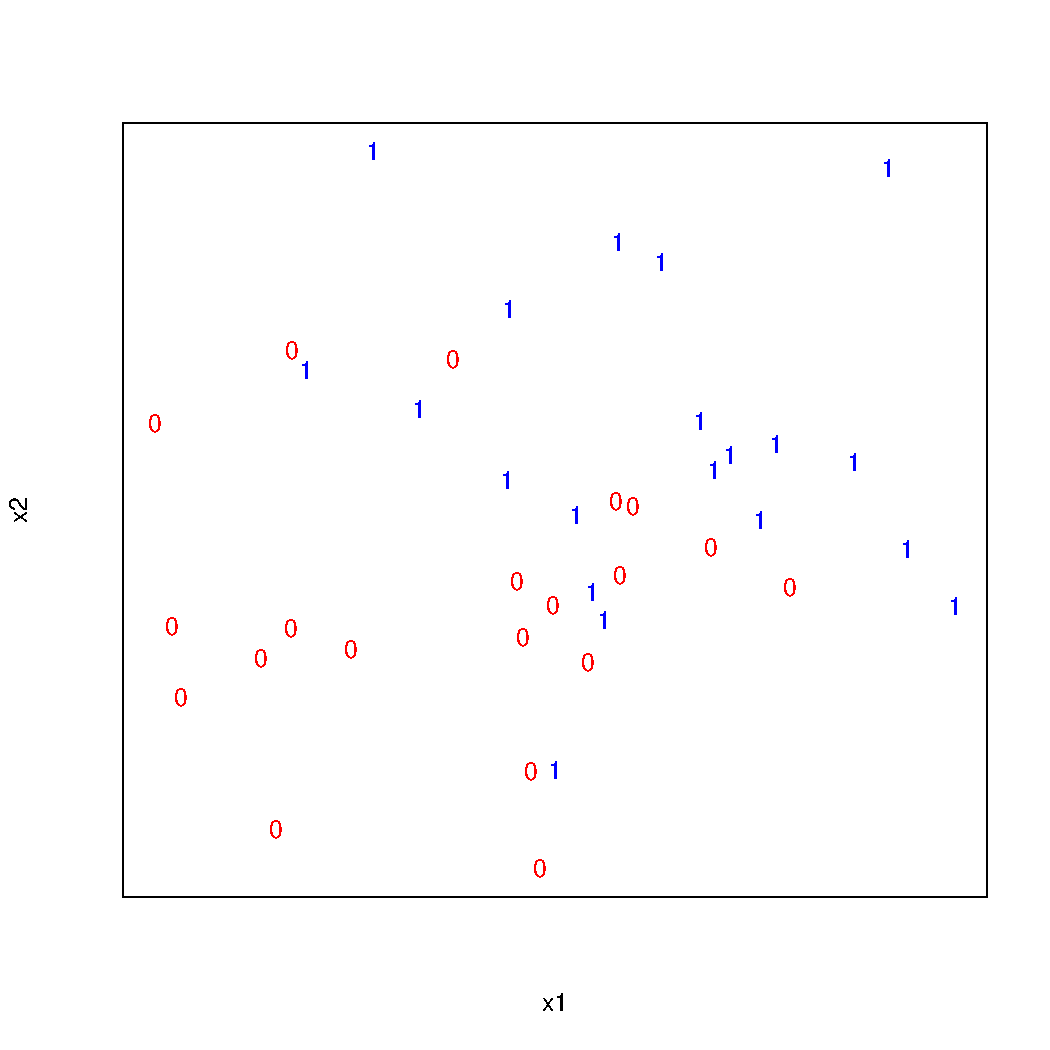
\includegraphics[width=.6\linewidth]{figure/beamer-predmod4-1} 

}



\end{knitrout}
\end{frame}

\begin{frame}
  \frametitle{Less Clear-cut case}
\begin{knitrout}\tiny
\definecolor{shadecolor}{rgb}{0.969, 0.969, 0.969}\color{fgcolor}

{\centering 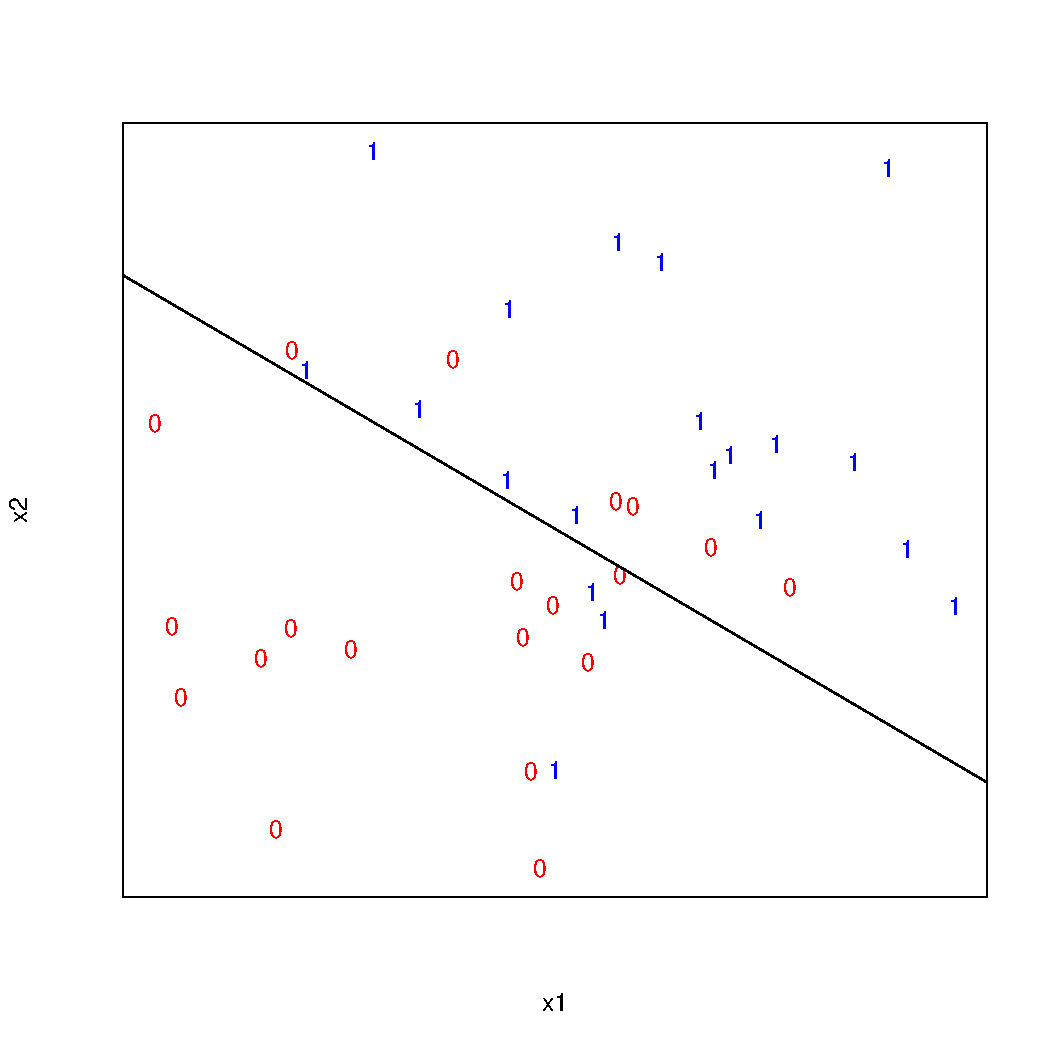
\includegraphics[width=.6\linewidth]{figure/beamer-predmod5-1} 

}



\end{knitrout}
\end{frame}

\begin{frame}
  \frametitle{Less Clear-cut case}
\begin{knitrout}\tiny
\definecolor{shadecolor}{rgb}{0.969, 0.969, 0.969}\color{fgcolor}

{\centering 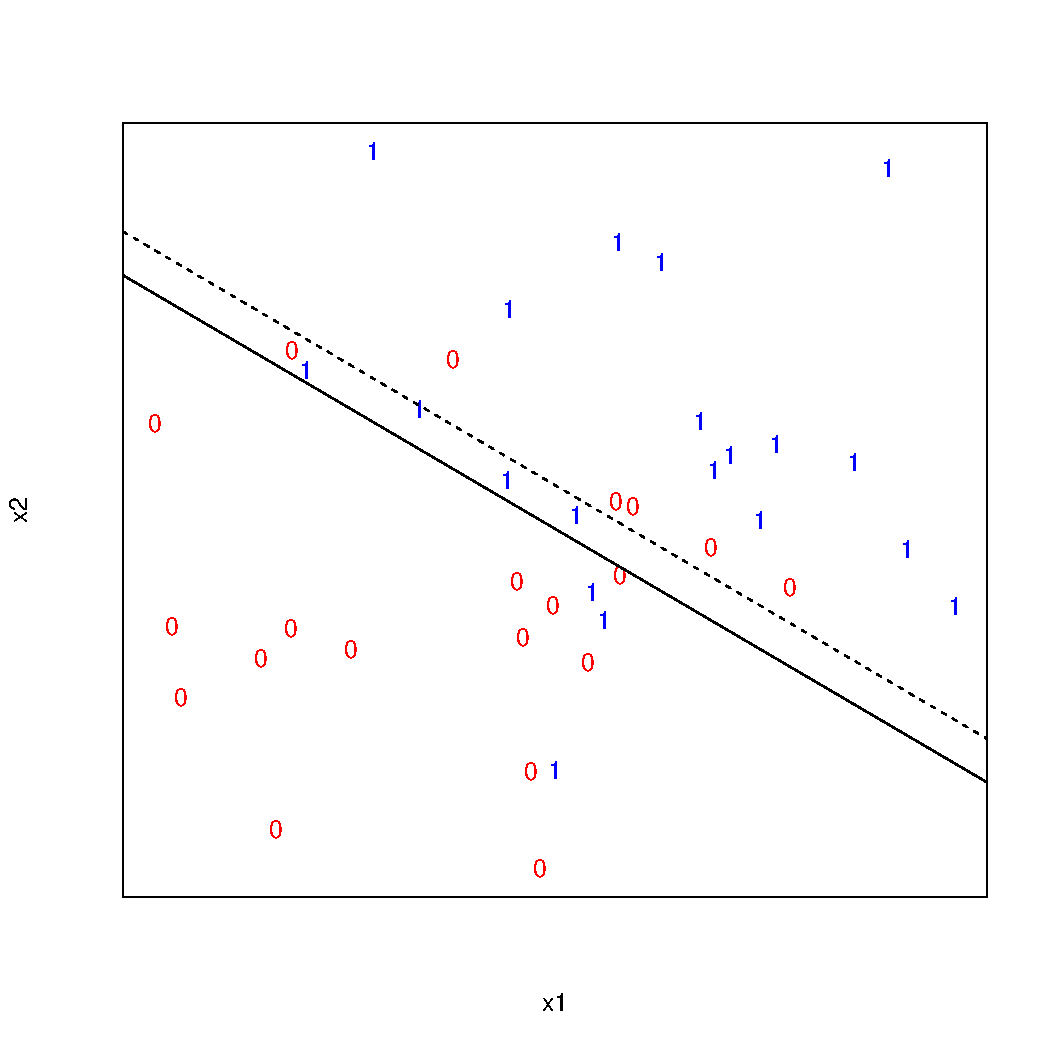
\includegraphics[width=.6\linewidth]{figure/beamer-predmod6-1} 

}



\end{knitrout}
\end{frame}


\begin{frame}[plain]
  \frametitle{Regression Problem}
\begin{figure}
\centering
\begin{knitrout}\tiny
\definecolor{shadecolor}{rgb}{0.969, 0.969, 0.969}\color{fgcolor}

{\centering 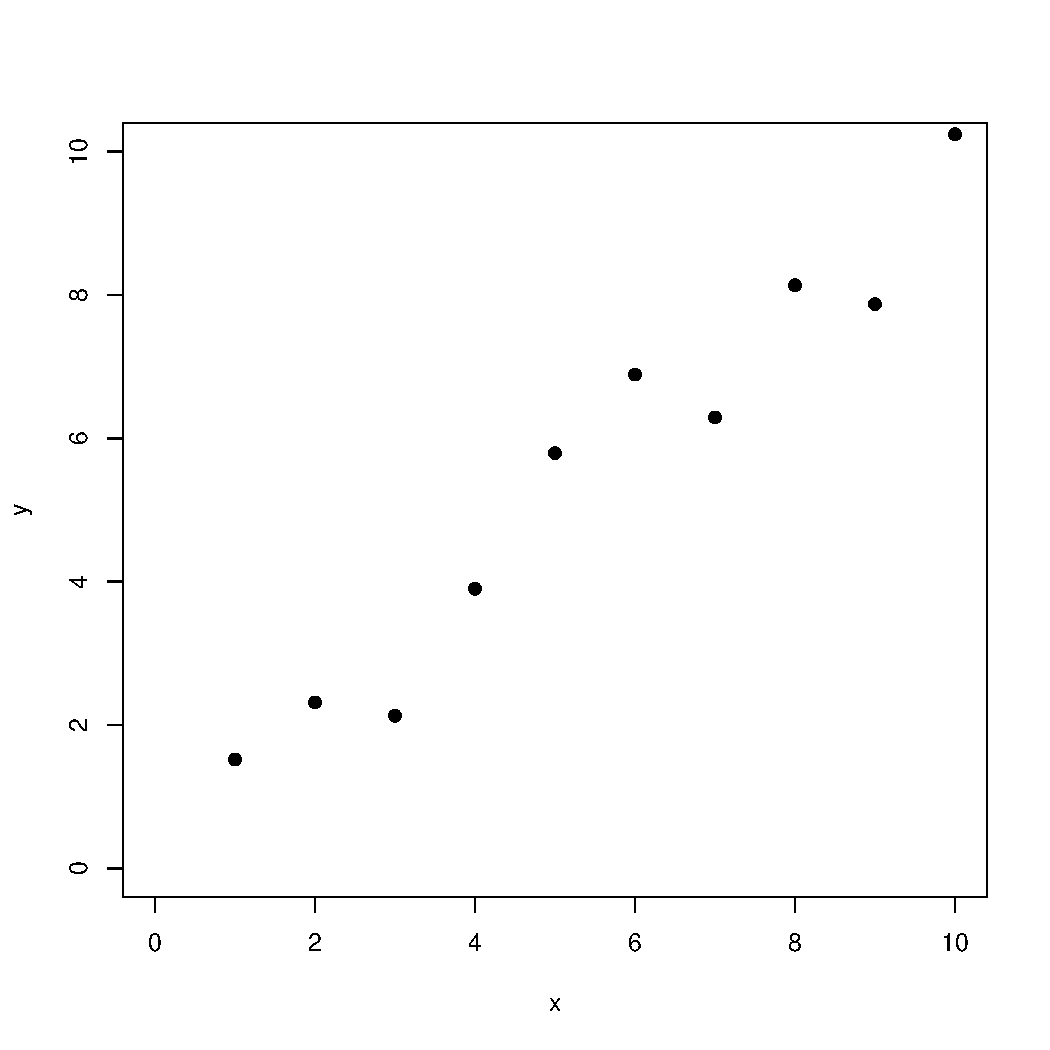
\includegraphics[width=.6\linewidth]{figure/beamer-unnamed-chunk-40-1} 

}



\end{knitrout}
\end{figure}
\end{frame}

\begin{frame}[plain]
  \frametitle{Linear Regression (lin)}
\begin{figure}
\centering
\begin{knitrout}\tiny
\definecolor{shadecolor}{rgb}{0.969, 0.969, 0.969}\color{fgcolor}

{\centering 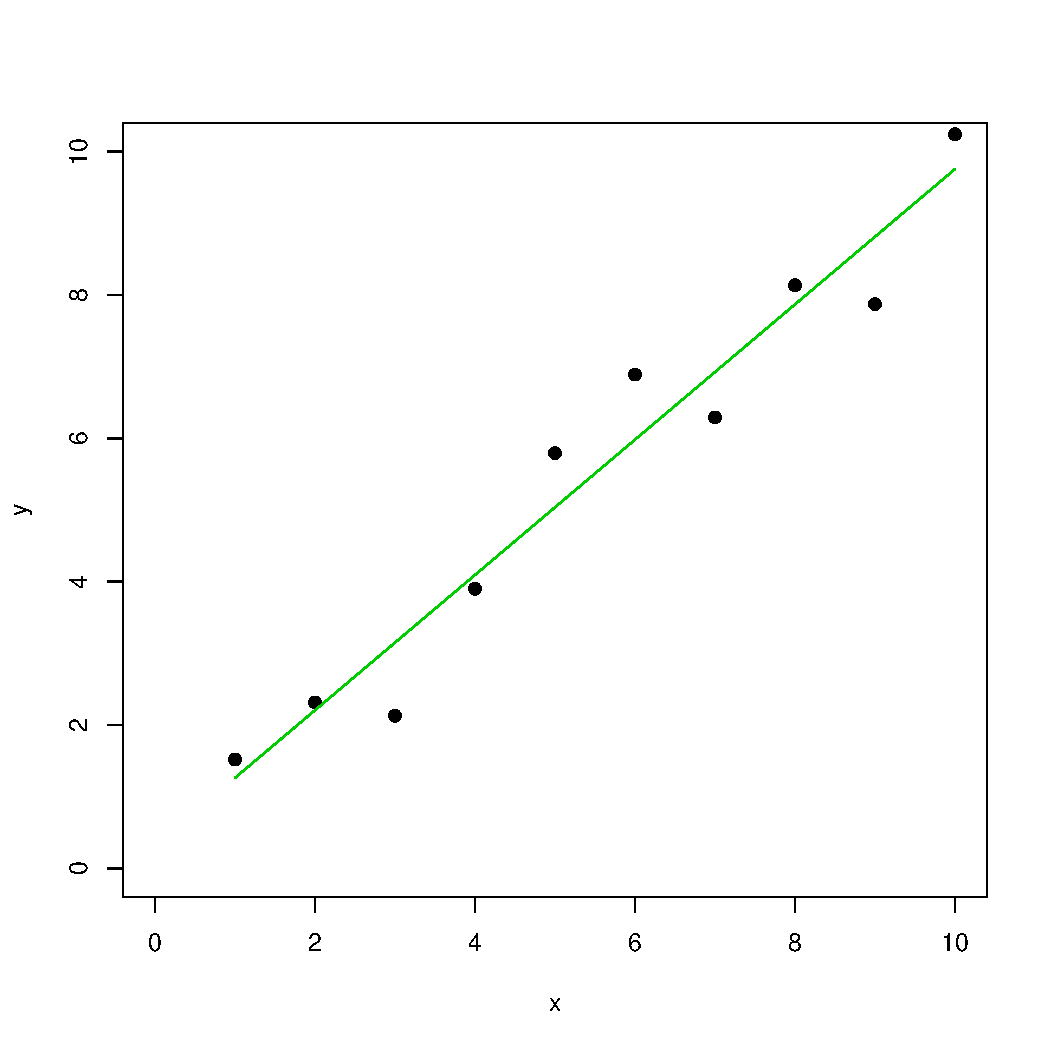
\includegraphics[width=.6\linewidth]{figure/beamer-unnamed-chunk-41-1} 

}



\end{knitrout}
\end{figure}
\end{frame}

\begin{frame}[plain]
  \frametitle{Spline Regression (spl)}
\begin{figure}
\centering
\begin{knitrout}\tiny
\definecolor{shadecolor}{rgb}{0.969, 0.969, 0.969}\color{fgcolor}

{\centering 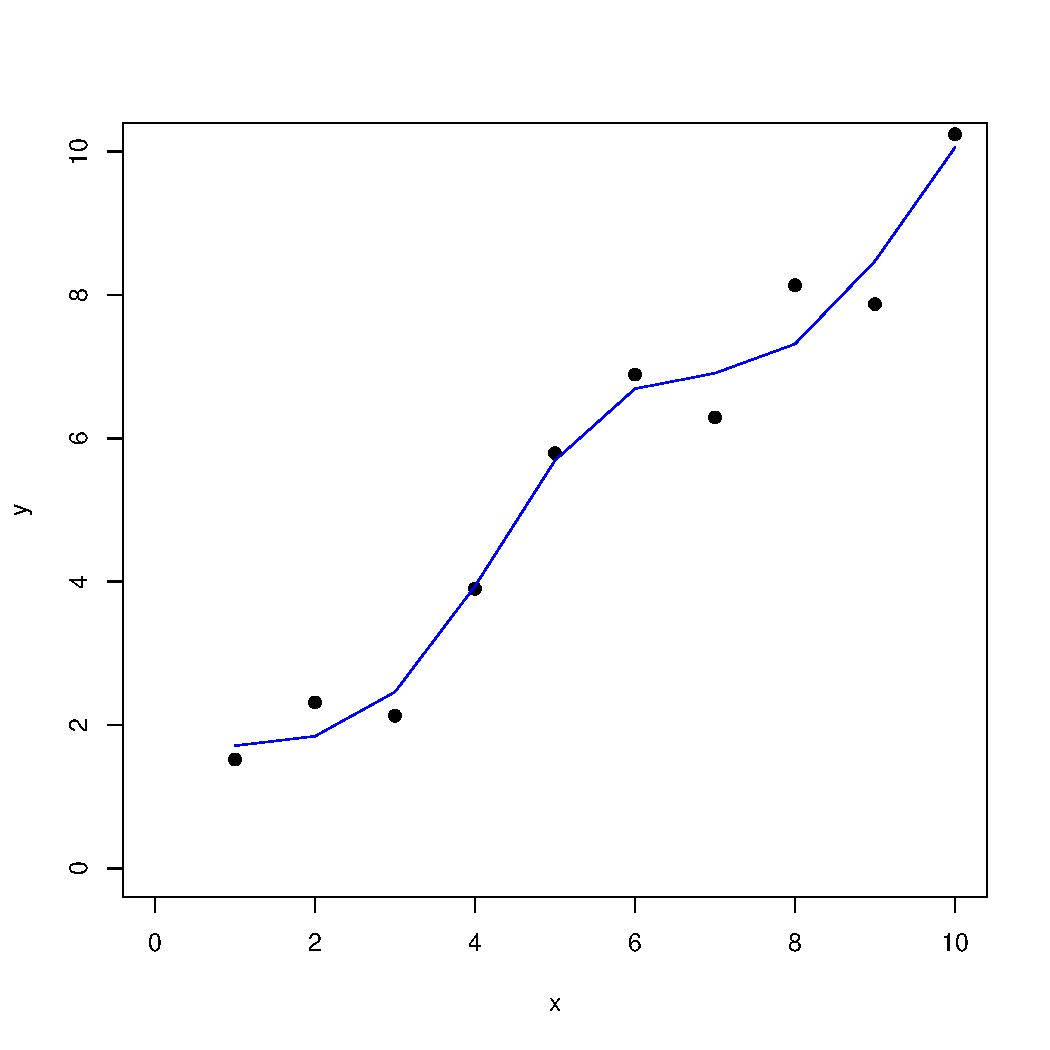
\includegraphics[width=.6\linewidth]{figure/beamer-unnamed-chunk-42-1} 

}



\end{knitrout}
\end{figure}
\end{frame}

\begin{frame}[plain]
  \frametitle{Connect the dots (ctd)}
\begin{figure}
\centering
\begin{knitrout}\tiny
\definecolor{shadecolor}{rgb}{0.969, 0.969, 0.969}\color{fgcolor}

{\centering 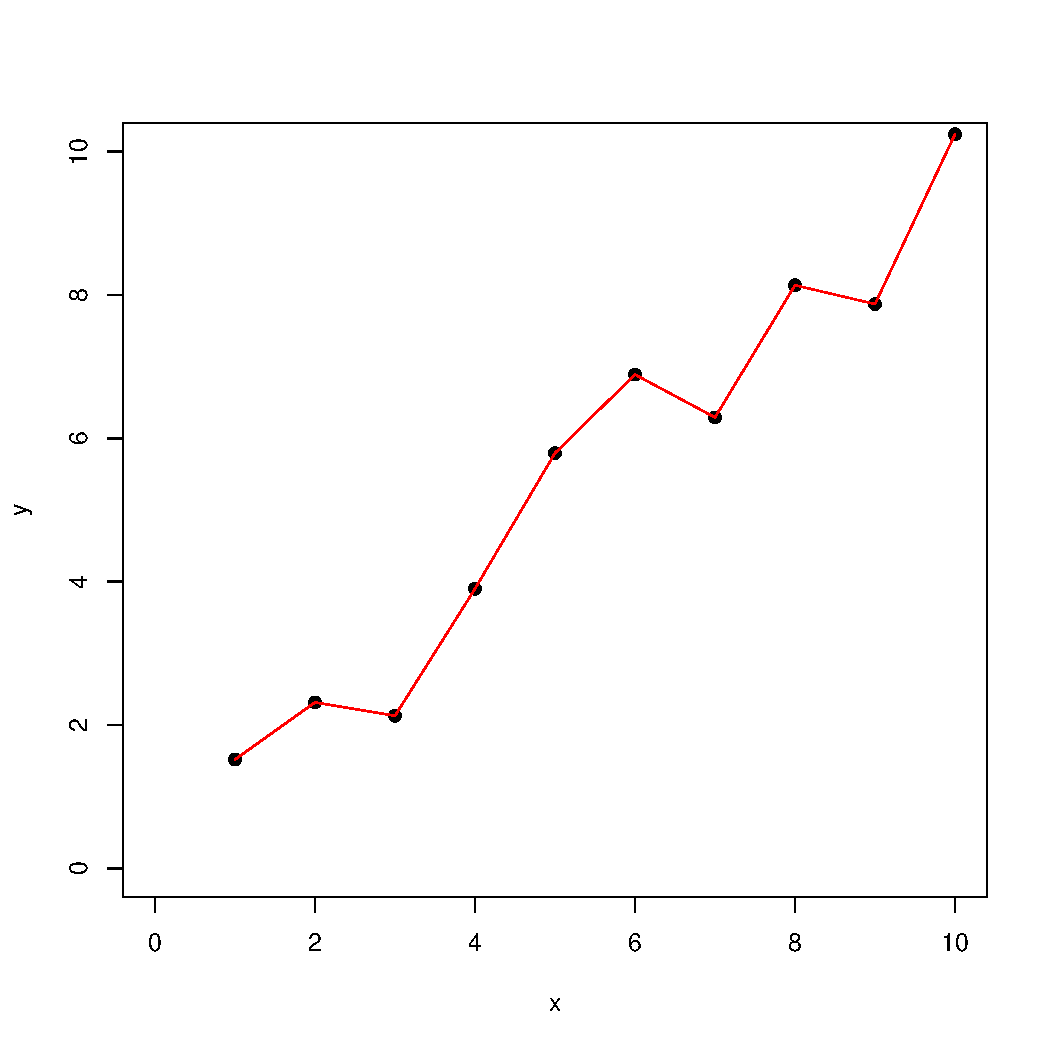
\includegraphics[width=.6\linewidth]{figure/beamer-unnamed-chunk-43-1} 

}



\end{knitrout}
\end{figure}
\end{frame}
\begin{frame}[plain]
  \frametitle{Which Approach?}
\begin{figure}
\centering
\begin{knitrout}\tiny
\definecolor{shadecolor}{rgb}{0.969, 0.969, 0.969}\color{fgcolor}

{\centering 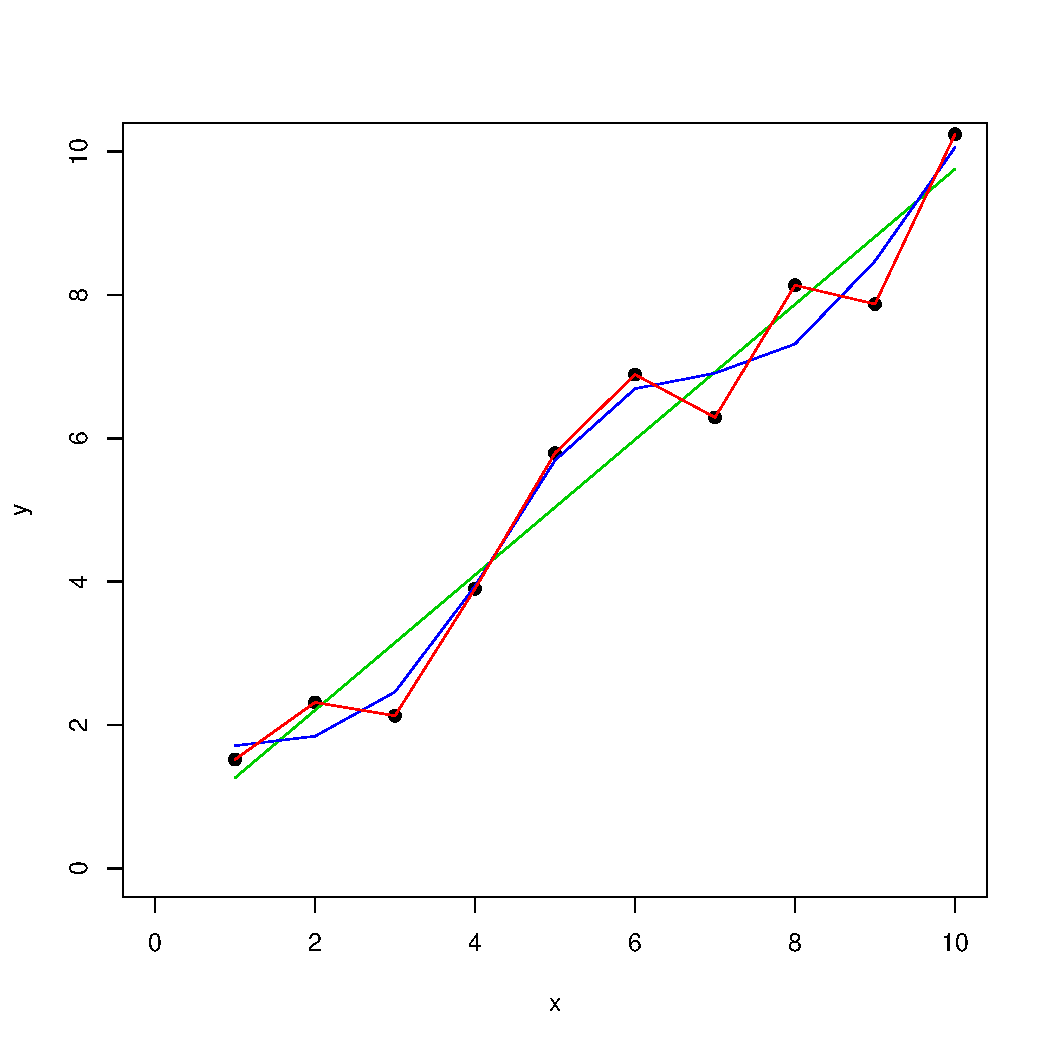
\includegraphics[width=.6\linewidth]{figure/beamer-unnamed-chunk-44-1} 

}



\end{knitrout}
\end{figure}
\end{frame}


\begin{frame}
  \frametitle{Supervised Learning (Classification)}
  \begin{itemize}
\item Goal: Predict a binary outcome ($Y$) on the basis of 
      baseline information ($X$)
\item $Y$ assumes the value 0 or 1 (e.g., control vs case, or AML vs ALL)
\item $X$ could be single variable or be a vector of multiple variables
\item Example: Can you predict $Y$ on the basis of two genes say $X_1$ and $X_2$
\item Note that a goal is to build a machine that will take on two values $X_1$ and $X_2$
      and return a 0 or a 1
\item You can denote this machine as a function $g(x_1,x_2)$
\end{itemize}
\end{frame}

\begin{frame}
  \frametitle{Classifier}
  \begin{itemize}
\item We will denote the predictor or classifier by $g(x)$
\item $x=(x_1,x_2)$ is the vector of gene expressions for genes 1 and 2
\item Based on $x$, the classifier $g$ makes a prediction for the outcome
\item Note that $g(x)=0$ or $g(x)=1$
\item The prediction is {\it correct} if $Y=1$ and $g(x_1,x_2)=1$, or $Y=0$ and $g(x_1,x_2)=0$
\item The prediction is {\it wrong} if $Y=0$ and $g(x_1,x_2)=1$, or $Y=1$ and $g(x_1,x_2)=0$
\end{itemize}
\end{frame}


\begin{frame}
  \frametitle{Prediction Assessment}
\begin{table}
\centering
  \begin{tabular}{ccc}
       &$g(x_1,x_2)=0$&$g(x_1,x_2)=1$\\
  $Y=0$&True-Negative&False-Negative\\
  $Y=1$&False-Negative&True-Positive
  \end{tabular}
\end{table}
\end{frame}



\begin{frame}{Steps to Construct a Classifier}
  \begin{itemize}
  \item Collect a random data set of size $n$ to build (train) a classifer 
  \item This is called the training data
  \item On the basis of these data, construct the classifier $g_n$
  \item It is subscripted by $n$ to emphasize that it is trained on the
        basis of the training data
  \item Note that the final performance of $g_n$ is {\it not} 
         be judged on the basis of the training data
  \item It is to be judged on the basis of its performance on {\it future} data
  \item Called testing data
  \end{itemize}
\end{frame}


\begin{frame}{Steps in Notation}
  \begin{itemize}
  \item Collect the training data $(X_1,Y_1),\ldots,(X_n,Y_n)$
  \item Construct a classifier $g_n$ on the basis of the training data
  \item Apply $g_n$ to a new data set $X^*_1,\ldots,X_k^*$ to get
  \item $k$ predictions: $\hat{Y}_1^*,\ldots,\hat{Y}_k^*$
  \item Compare the predictions to the observed outcomes $Y^*_1,\ldots,Y^*_k$
  \item Note that at the testing stage, you are blinded to the $Y^*_k$
  \end{itemize}
\end{frame}





%% \begin{frame}
%%   \frametitle{$k$-Nearest Neighborhood (Non-parametric)}
%%   \begin{itemize}
%%   \item The last two methods are parametric: you assume that you know the
%%         functional form of the regression function up to three unknown parameters 
%%   \item In an microarray experiment, it may not be appropriate to make strong
%%         parametric assumptions
%%   \item Non-parametric methods (e.g., $k$-NN) are preferred.
%%   \item For each $x$ (point on the scatter plot), identify the $k$ nearest neighbors
%%   \item Among the $k$ neighbors, count the number of responders (say $r_x$)
%%   \item Set
%%     \begin{equation*}
%%       \hat{\eta}(x)=\frac{r_x}{k}
%%     \end{equation*}
%%   \end{itemize}
%% \end{frame}


\begin{frame}
  \frametitle{k-Nearest Neighborhood}
\begin{knitrout}\tiny
\definecolor{shadecolor}{rgb}{0.969, 0.969, 0.969}\color{fgcolor}

{\centering 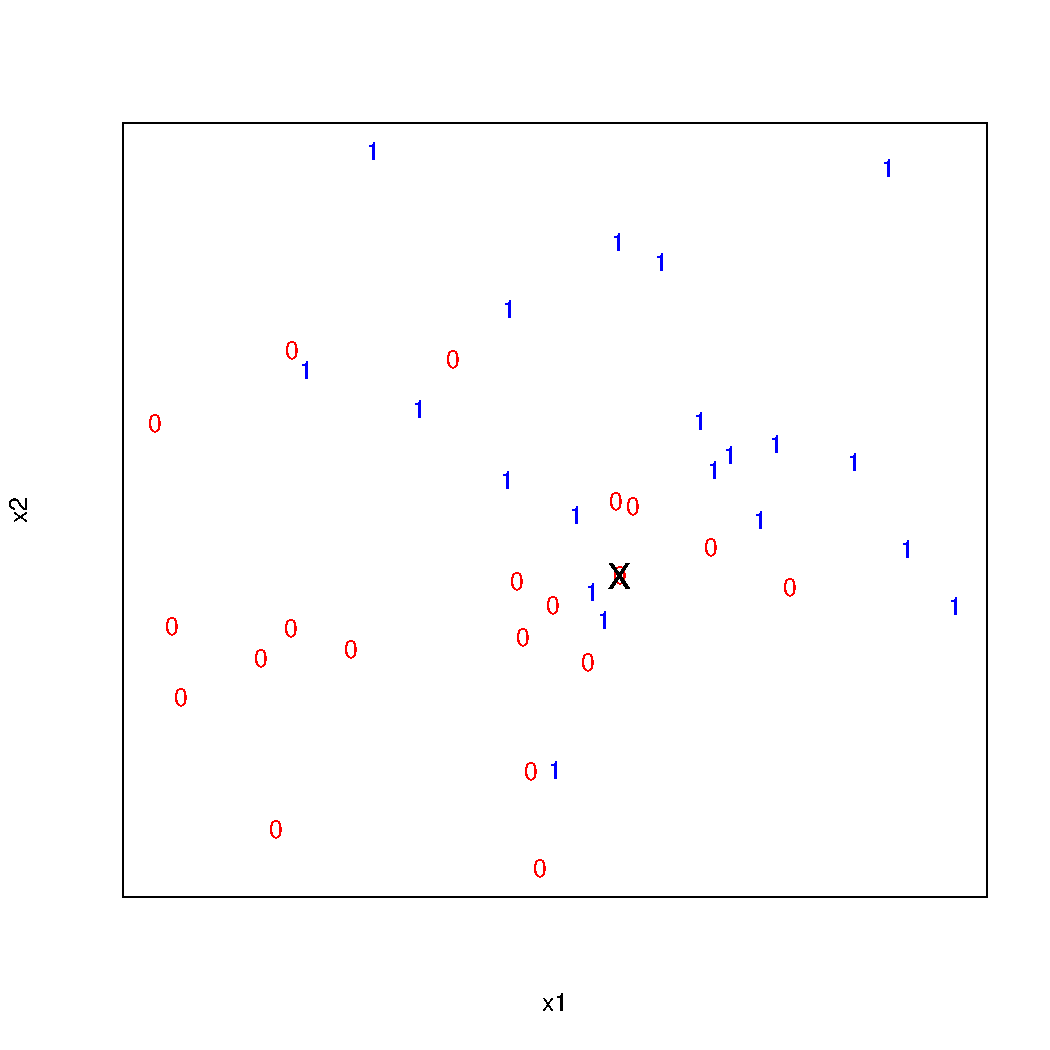
\includegraphics[width=.6\linewidth]{figure/beamer-knn-1} 

}



\end{knitrout}
\end{frame}


\begin{frame}
  \frametitle{3-Nearest Neighborhood}
\begin{knitrout}\tiny
\definecolor{shadecolor}{rgb}{0.969, 0.969, 0.969}\color{fgcolor}

{\centering 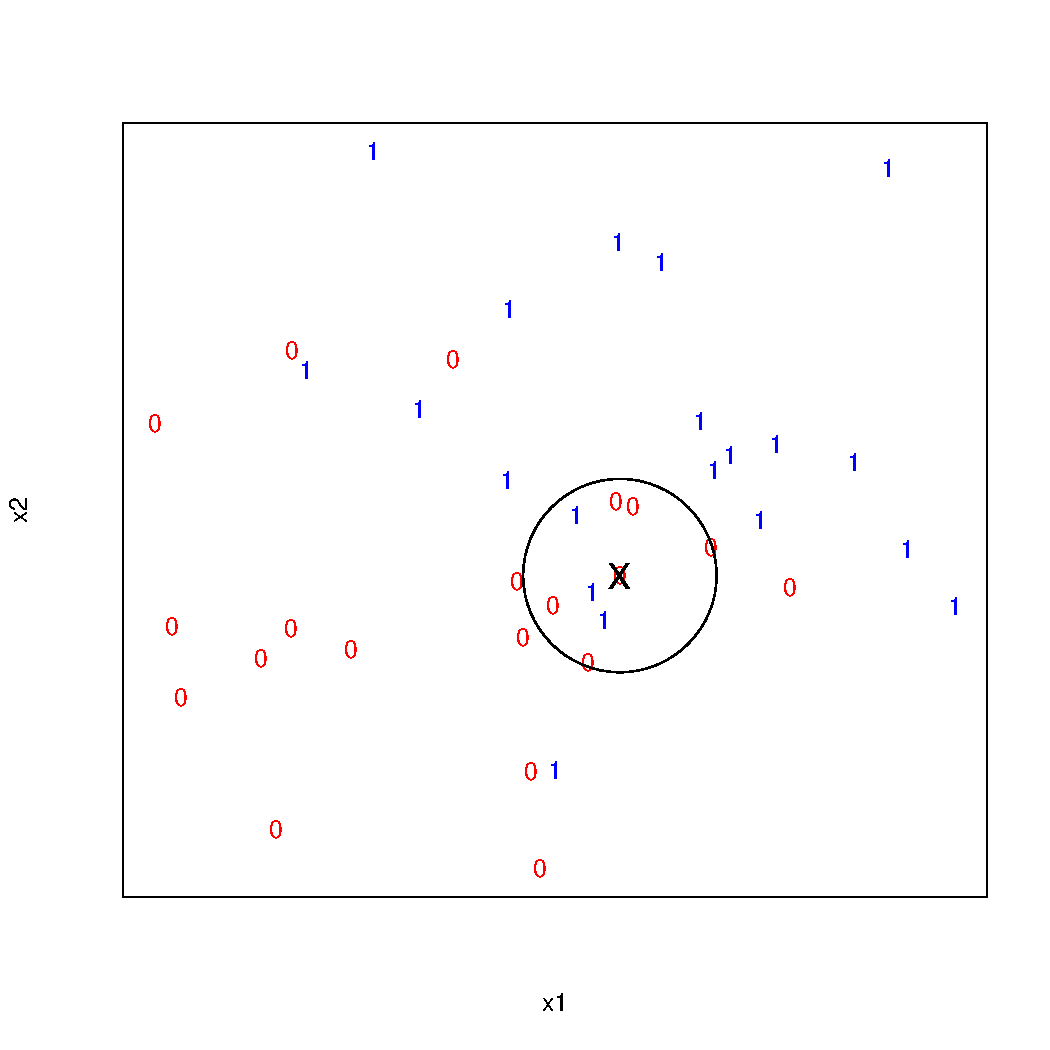
\includegraphics[width=.6\linewidth]{figure/beamer-knn3-1} 

}



\end{knitrout}
\end{frame}

\begin{frame}
  \frametitle{5-Nearest Neighborhood}
\begin{knitrout}\tiny
\definecolor{shadecolor}{rgb}{0.969, 0.969, 0.969}\color{fgcolor}

{\centering 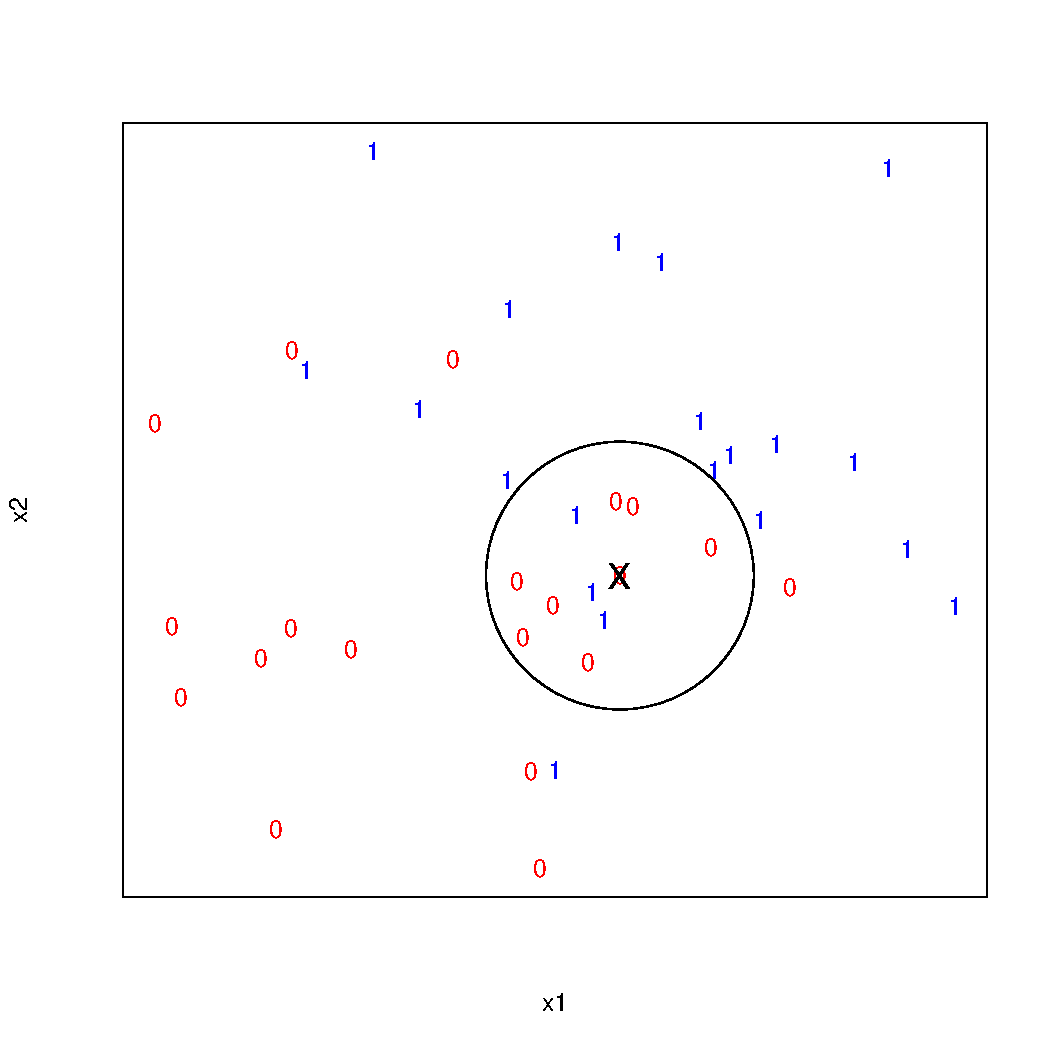
\includegraphics[width=.6\linewidth]{figure/beamer-knn5-1} 

}



\end{knitrout}
\end{frame}




%% \begin{frame}
%%   \frametitle{Mean Regression Model}
%%   \begin{itemize}
%%   \item $ E(Y)$ is the {\it unconditional} (on $X$) mean of $Y$. 
%%   \item Model the mean relationship between $Y$ and $X$
%%     \begin{equation*}
%%       \eta(x)=E(Y|X=x)
%%     \end{equation*}
%%   \item $\eta(x)$ is the {\it conditional} (on $X$) mean of $Y$ given that $X$ has realized the value $x$.
%%   \end{itemize}
%% \end{frame}

%% \begin{frame}
%%   \frametitle{Bayes Classifier}
%%   \begin{equation*}
%%     g(X)=
%%     \begin{cases}
%%       1&\mbox{ if } \eta(X)\ge \frac{1}{2},\\
%%       0&\mbox{ if } \eta(X)< \frac{1}{2}
%%     \end{cases}
%%   \end{equation*}
%%   \begin{itemize}
%%   \item This classifier is "optimal" in the sense that there is no better classifier
%%         with respect to minimizing the error ($P(g(X)\ne Y)$).
%%   \item Suppose that $g^*$ is another classifier. Then 
%%     \begin{equation*}
%%       P(g(X)\ne Y) \le  P(g^*(X)\ne Y)
%%     \end{equation*}
%%   \item Note that the optimality concerns $\eta(x)$ and not $\hat{\eta}(x)$.
%%   \end{itemize}
%% \end{frame}




%% \begin{frame}
%%   \frametitle{Logistic Regression (Parametric)}
%%   \begin{itemize}
%%   \item Most commonly used method for modeling the relationship between
%%         a binary response and a set of co-variables
%%   \begin{equation*}
%%     \mathrm{logit}(\eta(x))=\beta_0 + \beta_1 x_1 + \beta_2 x_2,
%%   \end{equation*}
%%   where 
%%   \begin{equation*}
%%     \mathrm{logit}(\eta(x))=\log\bigg(\frac{p}{1-p}\bigg),
%%   \end{equation*}
%% for $p\in (0,1)$ is called the "logit" function.
%% \end{itemize}
%% \end{frame}

%% \begin{frame}
%%   \frametitle{Estimating $\eta(x)$}
%%   \begin{itemize}
%%    \item Estimate the model parameters  ($\beta_0,\beta_1$ and
%% $\beta_2$) using maximum-likelihood estimation to get
%%   $\hat{\beta}_0,\hat{\beta}_1$ and $\hat{\beta}_2$
%% \item For the logistic model
%%   \begin{equation*}
%%     \hat{\eta}(x)=\frac{\exp(\hat{\beta}_0+\hat{\beta}_1x_1+\hat{\beta}_2x_2)}{1+\exp(\hat{\beta}_0+\hat{\beta}_1x_1+\hat{\beta}_2x_2)}
%%   \end{equation*}
%% \end{itemize}
%% \end{frame}





%% <<echo=FALSE>>=
%% rm(n,x0,x1)
%% @ 


%% \begin{frame}
%%   \frametitle{Other Classification Methods}
%%   \begin{itemize}
%% \item Fisher's Linear Discriminant
%%  \item Support Vector Machines (SVM)
%%   \item Classification and Regression Trees (CART)
%%   \item Random Forests (aggregated trees)
%%   \end{itemize}
%% \end{frame}

%% \begin{frame}
%%   \frametitle{Bias versus Variance}
%%   \begin{itemize}
%% \item A very important principle in statistical modeling is the so called {\it bias-variance tradeoff}
%% \item The bias of $\hat{\eta}(x)$ is
%%   \begin{equation*}
%%     b(x)=\hat{\eta}(x)-\eta(x)
%%   \end{equation*}
%% \item The variance of $\hat{\eta}(x)$ is
%%     \begin{equation*}
%%     v(x)=E(\hat\eta(x)-\eta(x))^2)
%%   \end{equation*}
%% \item The bias-variance tradeoff implies that both cannot be minimized simultaneously
%% \item For example for the $k$-NN method increasing $k$ increases bias while decreasing variance
%%   \end{itemize}
%% \end{frame}


%% \begin{frame}
%%   \frametitle{Training and Testing}
%%   \begin{itemize}
%%   \item In practice, the model is first estimated (trained) using an initial set of data
%%   \item This data set is usually called the "training" data
%%   \item Once the model is trained, then it is applied to an "independent" set of data
%%   \item This data set is usually called the "testing" (or validation) data set
%%   \end{itemize}
%% \end{frame}








\begin{frame}
  \frametitle{Parsimony}
  \begin{itemize}
\item The model should be parsimonious (less is more)
\item Including too many noisy/unimportant 
      features often degrades the performance of the classifier.
\item Including highly dependent induces problems (e.g., multi-collinearity from simple linear regression).
\item Additional complication:
      It is not practically/computationally feasible to include tens of thousands
      of features in the model. 
\end{itemize}
\end{frame}

\begin{frame}
  \frametitle{Overfitting}
  \begin{itemize}
\item Two many parameters compared to the number of data points in the training set
\item A complicated model will fit the training set well
\item It will however perform poorly for an independent set. 
\end{itemize}
\end{frame}


\begin{frame}[plain]
  \frametitle{Overfitting}
\begin{figure}
\centering
\begin{knitrout}\tiny
\definecolor{shadecolor}{rgb}{0.969, 0.969, 0.969}\color{fgcolor}

{\centering 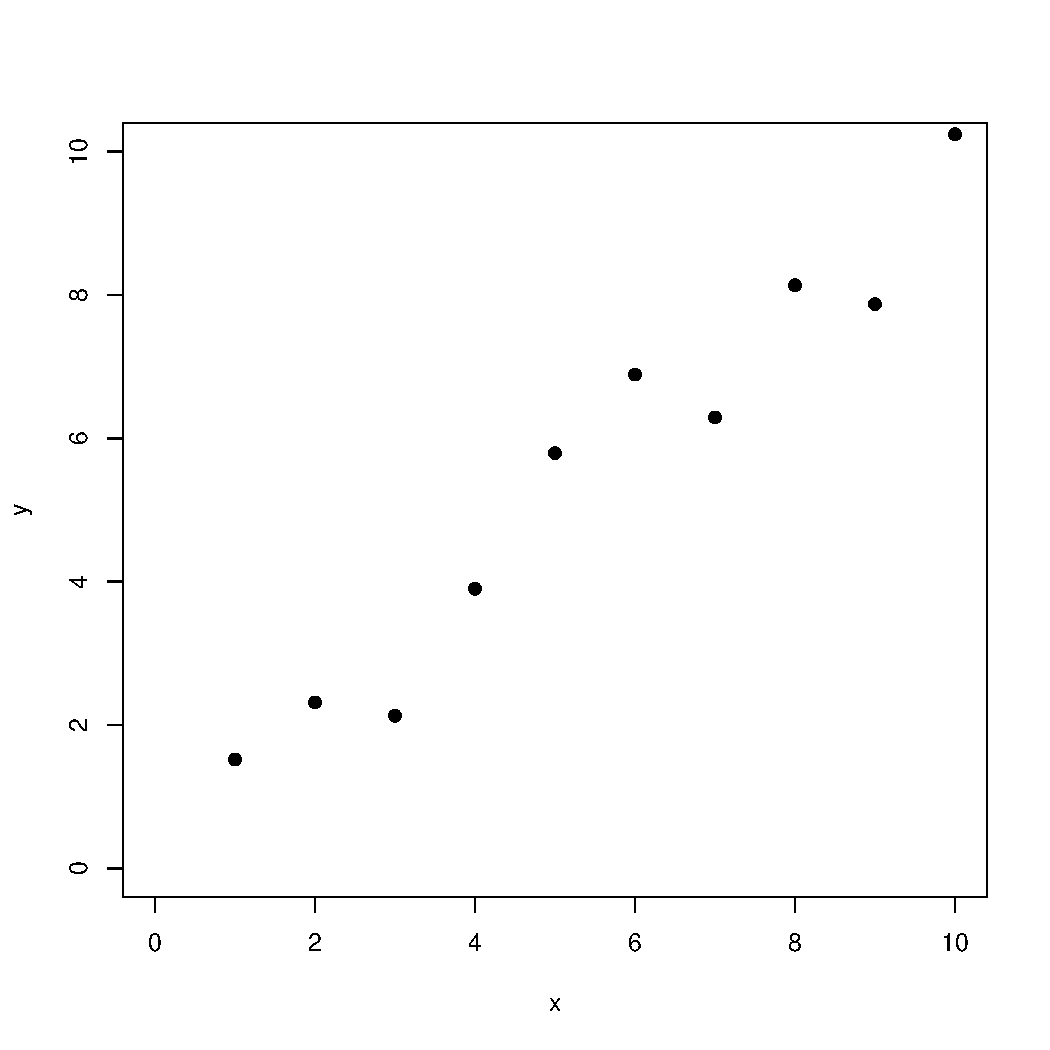
\includegraphics[width=.6\linewidth]{figure/beamer-unnamed-chunk-45-1} 

}



\end{knitrout}
\end{figure}
\end{frame}

\begin{frame}[plain]
  \frametitle{Linear Regression (lin)}
\begin{figure}
\centering
\begin{knitrout}\tiny
\definecolor{shadecolor}{rgb}{0.969, 0.969, 0.969}\color{fgcolor}

{\centering 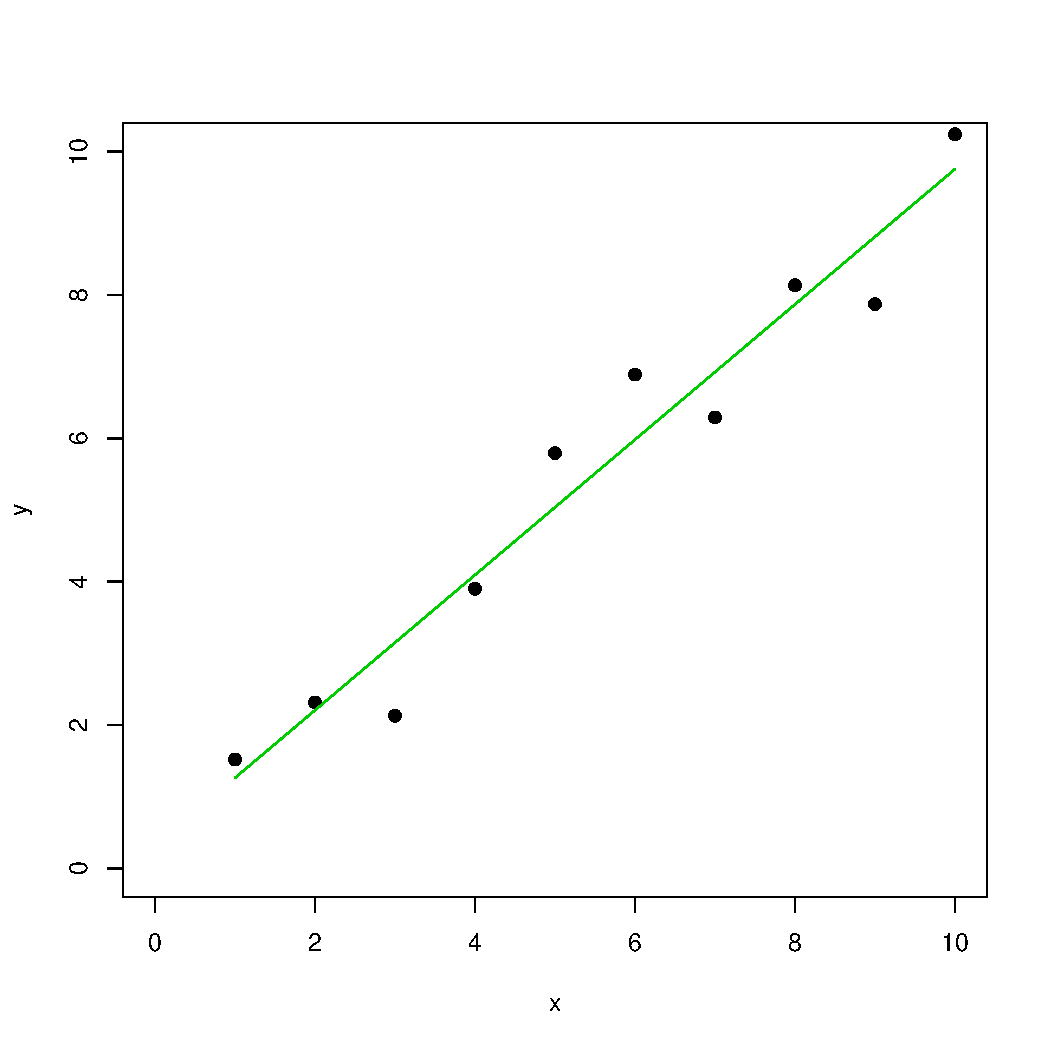
\includegraphics[width=.6\linewidth]{figure/beamer-unnamed-chunk-46-1} 

}



\end{knitrout}
\end{figure}
\end{frame}

\begin{frame}[plain]
  \frametitle{Spline Regression (spl)}
\begin{figure}
\centering
\begin{knitrout}\tiny
\definecolor{shadecolor}{rgb}{0.969, 0.969, 0.969}\color{fgcolor}

{\centering 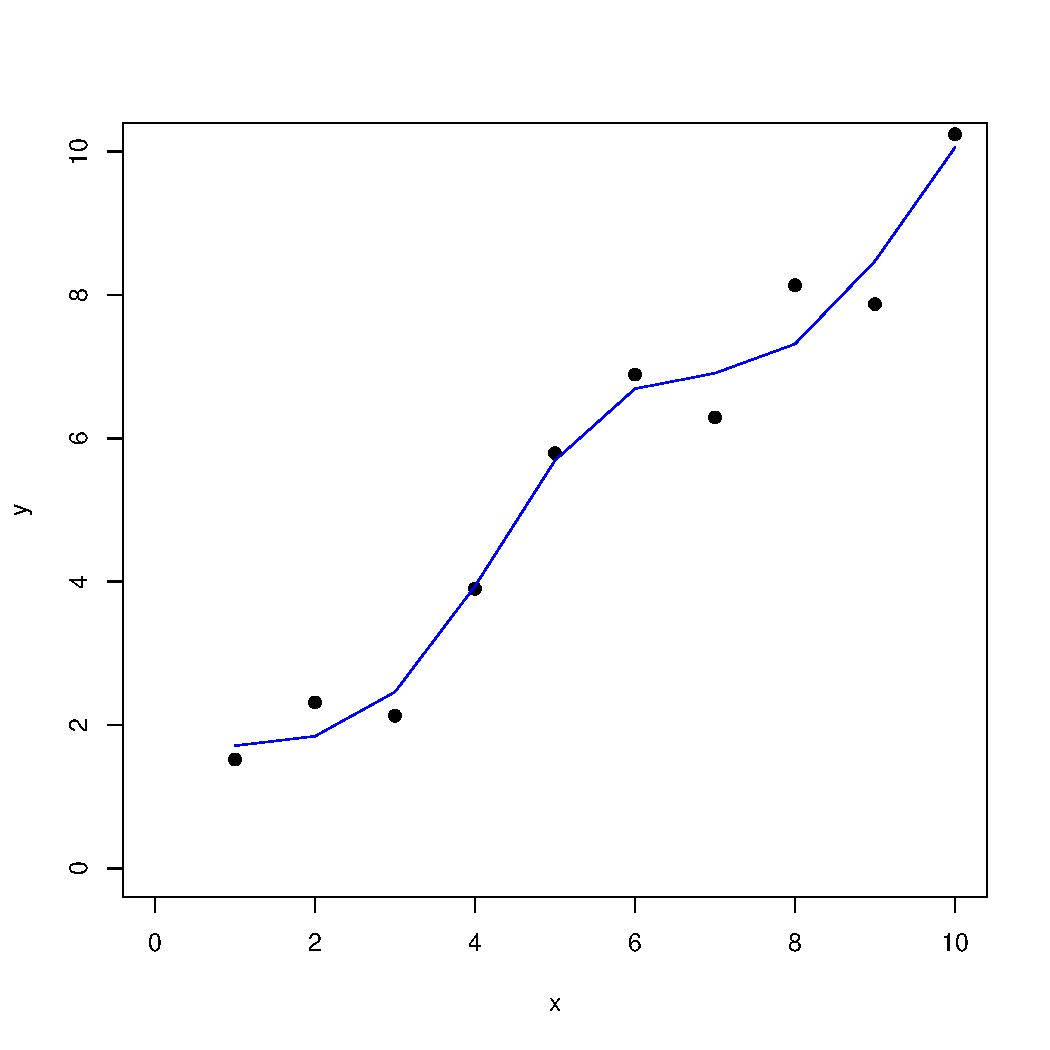
\includegraphics[width=.6\linewidth]{figure/beamer-unnamed-chunk-47-1} 

}



\end{knitrout}
\end{figure}
\end{frame}

\begin{frame}[plain]
  \frametitle{Connect the dots (ctd)}
\begin{figure}
\centering
\begin{knitrout}\tiny
\definecolor{shadecolor}{rgb}{0.969, 0.969, 0.969}\color{fgcolor}

{\centering 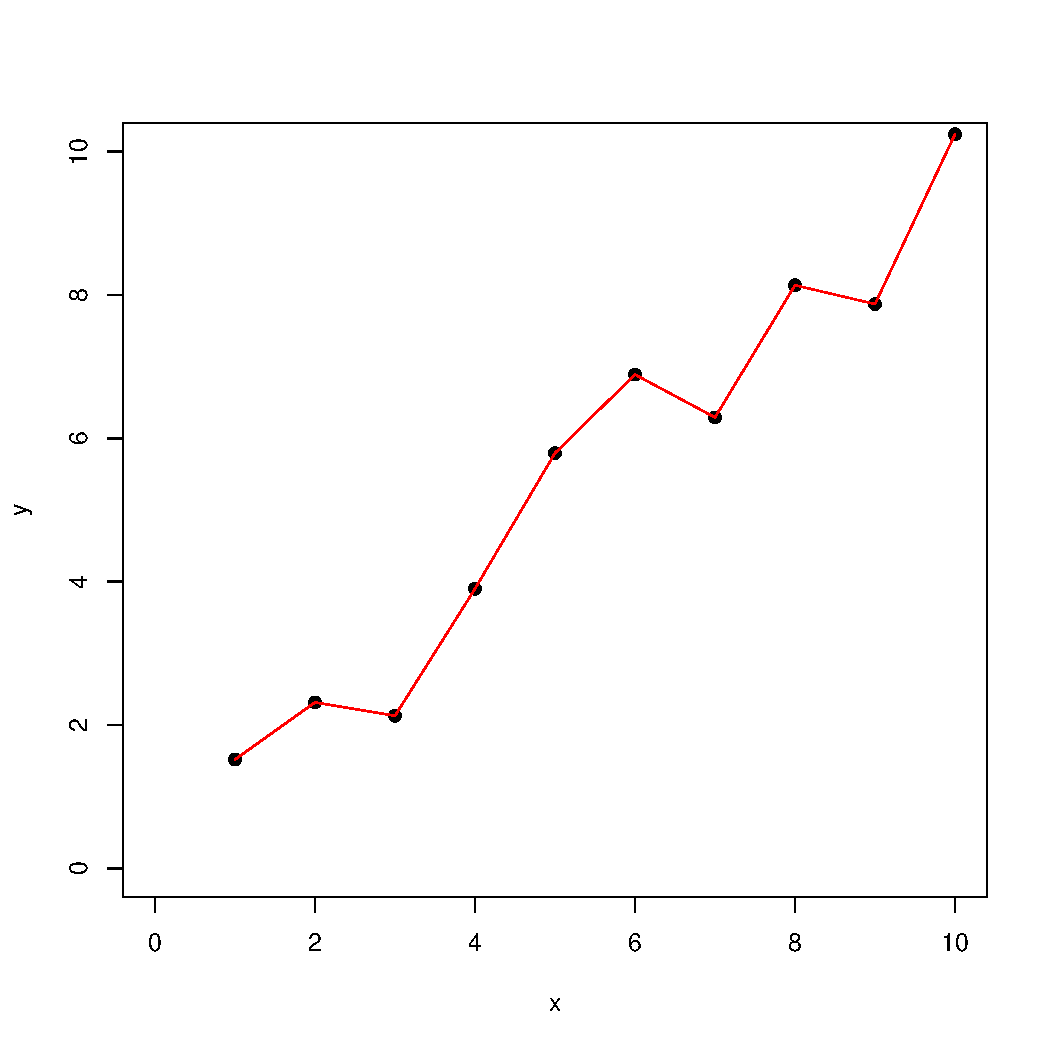
\includegraphics[width=.6\linewidth]{figure/beamer-unnamed-chunk-48-1} 

}



\end{knitrout}
\end{figure}
\end{frame}
\begin{frame}[plain]
  \frametitle{RSS: 4.1 (lin) vs 1.9 (spl) vs 0 (ctd)}
\begin{figure}
\centering
\begin{knitrout}\tiny
\definecolor{shadecolor}{rgb}{0.969, 0.969, 0.969}\color{fgcolor}

{\centering 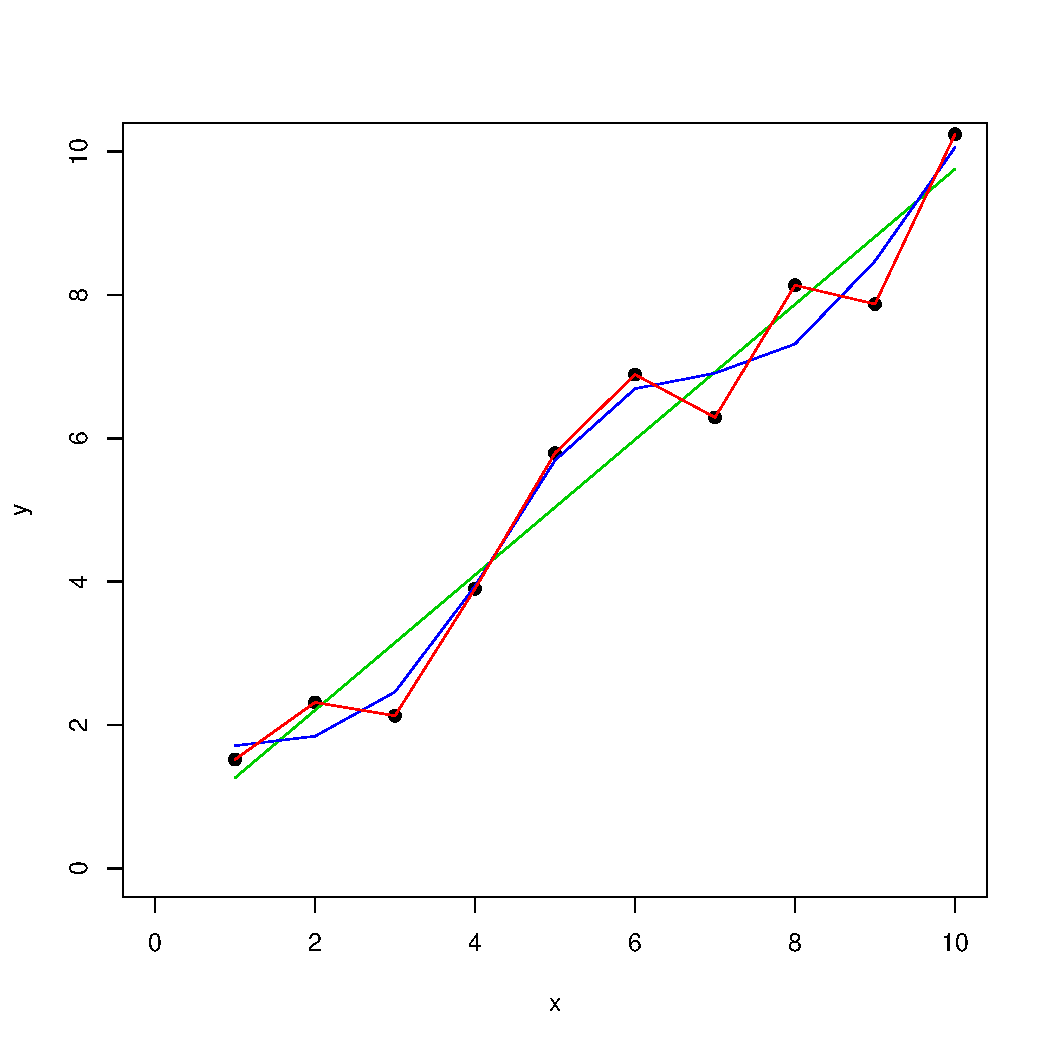
\includegraphics[width=.6\linewidth]{figure/beamer-unnamed-chunk-49-1} 

}



\end{knitrout}
\end{figure}
\end{frame}


\begin{frame}[plain]
  \frametitle{New Data Set}
\begin{figure}
\centering
\begin{knitrout}\tiny
\definecolor{shadecolor}{rgb}{0.969, 0.969, 0.969}\color{fgcolor}

{\centering 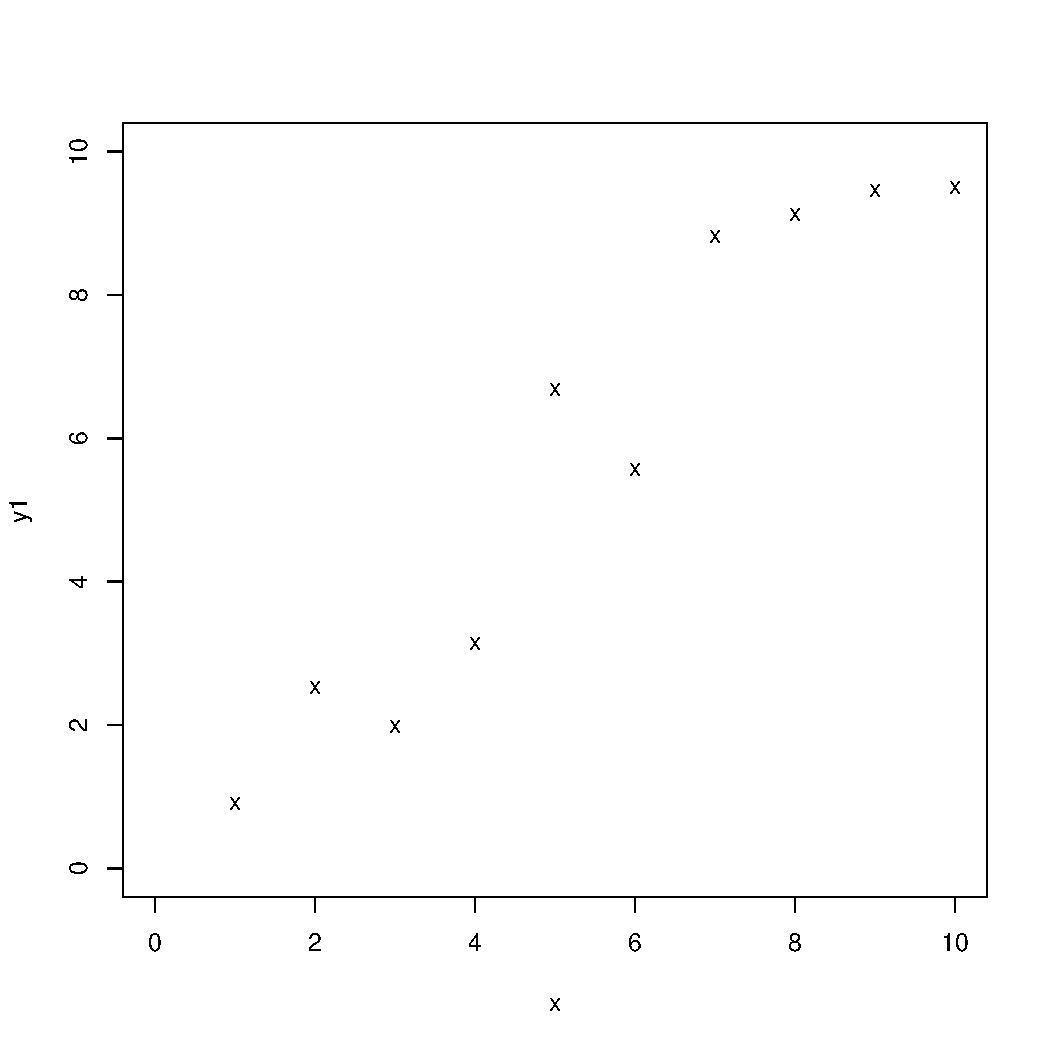
\includegraphics[width=.6\linewidth]{figure/beamer-unnamed-chunk-50-1} 

}



\end{knitrout}
\end{figure}
\end{frame}

\begin{frame}[plain]
  \frametitle{RSS: 11 (lin) vs 12.4 (spl) vs  14 (ctd)}
\begin{figure}
\centering
\begin{knitrout}\tiny
\definecolor{shadecolor}{rgb}{0.969, 0.969, 0.969}\color{fgcolor}

{\centering 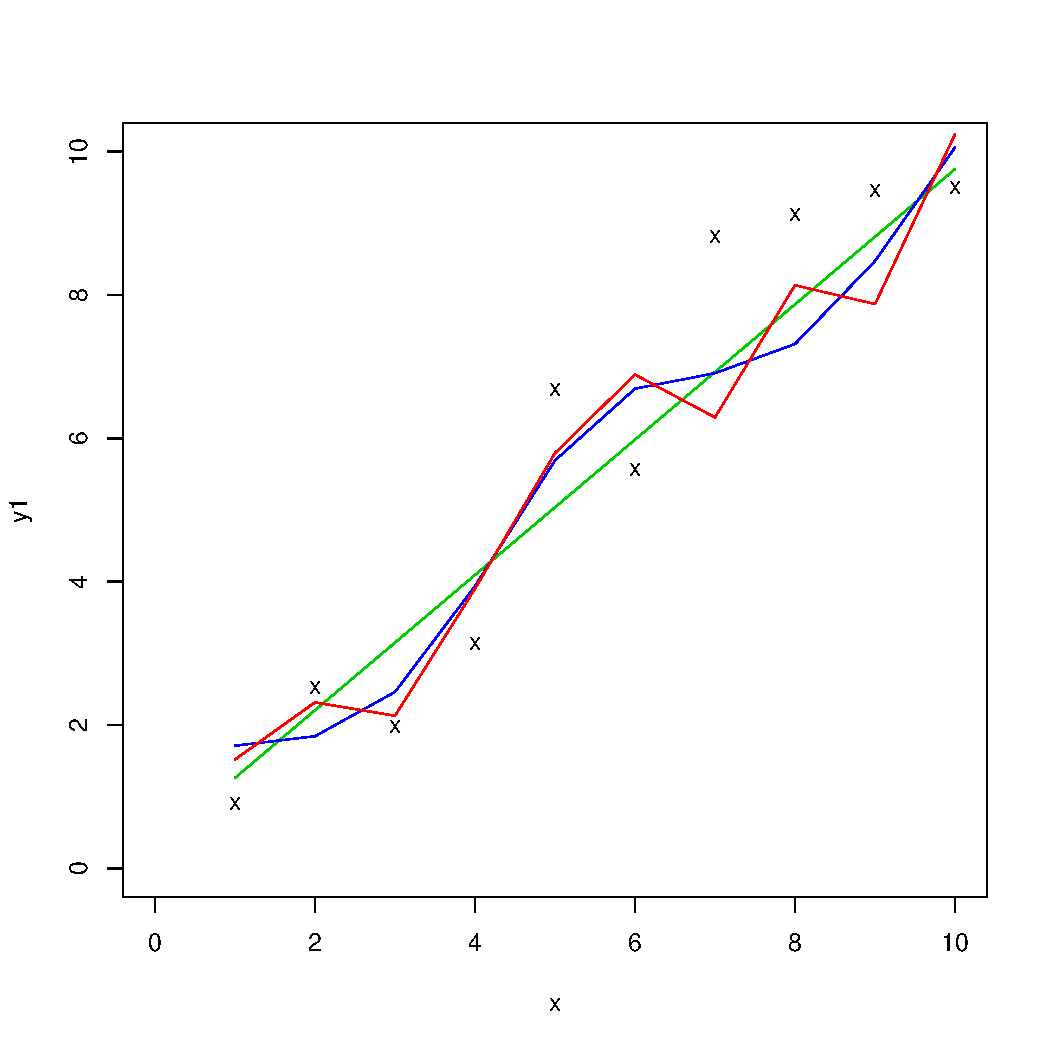
\includegraphics[width=.6\linewidth]{figure/beamer-unnamed-chunk-51-1} 

}



\end{knitrout}
\end{figure}
\end{frame}

\begin{frame}{Two Challenges in Building a Classifier}
  \begin{enumerate}
  \item Feature Selection:
    \begin{itemize}
    \item It is neither feasible nor provident to build a classifier based on all available
          variables
    \item A subset of the variables has to be selected to build the model
    \item This is also called feature extraction
    \end{itemize}
  \item Tuning Parameter Selection:
    \begin{itemize}
    \item Statistical methods may have one or more parameters that have to be set
    \item For example when using $k$-NN, one has to decide what $k$ should be (e.g., 1, 3 or 5 or how about 8)?
      \item Choosing the defaults set by the software is inappropriate  
    \item The feature selection method could also have tuning parameters that have to be set
          (e.g., the number of features to be selected)
    \item The performance of the method could be highly sensitive to the 
          choice of these parameters
    \end{itemize}
  \end{enumerate}
\end{frame}


\begin{frame}
  \frametitle{Feature Selection}
  \begin{itemize}
\item Reasonable Feature Selection is {\it critical} if not the most important
      component of model building.
\item You cannot expect to build a good model if you select poor features.      
\item This is also called Feature Extraction
\item We will talk about a few approaches that have been used in the literature.
\end{itemize}
\end{frame}


\begin{frame}
  \frametitle{Feature Selection (ranked based on test-statistic)}
  \begin{itemize}
\item Compute the two-sample t-test for all $m$ features (based on the training set) 
\item Identify the top say 10 or 15 features (e.g, ranked
      based on the absolute value of the test statistic).
\item Build a model on these "top" features (based on the training set) 
\item Alternatively, you could select all features for which the {\it P}-value is less
      than a certain threshold (say 0.001).
\item You can also use the Wilcoxon rank sum statistic to protect against choosing features
      with outliers.
\end{itemize}
\end{frame}





\begin{frame}
  \frametitle{Feature Selection (Ordination Methods)}
  \begin{itemize}
\item A standard approach for reducing the dimension in the microarray setting
      is the method of Principal Components (PCs)
\item The PCs are combinations of the original variables (gene expressions) that have maximum variability
\item The are also constructed as to be uncorrelated with another
\item This attempts to address the issue of high dimension and multi-collinearity simultaneously.
\item One can use the principal components (say the first two or three) as the features
\item Alternatively, one can first reduce the dimension by using the two-sample test-statistic approach
      and then get the PCs
\end{itemize}
\end{frame}


\begin{frame}
  \frametitle{Tuning}
  \begin{itemize}
\item You cannot expect to be able to build a model using default values provided by the software
      package.
\item If you use {\it k}-NN you need to decide which $k$ (e.g., 3 or 5 or 7) you want to use
\item If you use the simple feature selection method you need to determine how many "top" features you want 
      to use
\item If you are doing PC dimension reduction, you need to determine how many PCs you want to use.
\item In some books and articles, "tuning" only refers to the choice of the model parameter (e.g., $k$ in $k$-NN)
\item Must take a broader perspective as the choices in the FS part also affect the results.
\end{itemize}
\end{frame}



\begin{frame}
  \frametitle{Validation}
  \begin{itemize}
\item Split the data into a training and a mutually exclusive testing
      set
\item Build the model (including feature selection, tuning) on the
      {\it training} set
\item Evaluate the performance of the model
      on the {\it testing set}
\item IMPORTANT: The model is built based on the {\it training}
      set. The {\it testing} set should not contribute {\it any}
      information.
\item Violating this principle will invariably result in bias
\end{itemize}
\end{frame}

\begin{frame}
  \frametitle{Error Substitution Validation}
  \begin{itemize}
\item Error Substitution Validation: The testing set is empty. 
\item Test the model you just built on the {\it training} set
\item This approach cannot be recommended under any circumstance.
\item Analogy: Assess the fit of the linear model by plotting the
      fitted (from the data) to the observed data.
\item A bona-fide testing set is required.
\item Will demonstrate how this can lead to noise discovery
\end{itemize}
\end{frame}


\begin{frame}
  \frametitle{Hold-out Method}
  \begin{itemize}
\item Split the data into two parts
\item Keep the testing set locked up
\item Better yet, ask an "honest" broker to keep it from you until
      you are ready to test the model
\item This approach is reasonable if you have a large number of cases
\item It may be problematic if the outcomes are sparse

\end{itemize}
\end{frame}

\begin{frame}
  \frametitle{$k$-fold Cross-Validation}
  \begin{itemize}
\item Many microarray experiments are from smaller (e.g., pilot)
      studies
\item It is not impossible to get reasonably size training and testing
      sets this cases 
\item A reasonable approach to get around this is $k$-fold cross-validation (CV)
\item Randomly split cases into $k$ (nearly) equally sized subsets (folds).
\item At each step take of these $k$ portions as the {\it testing} set and 
      construct the {\it training} set based on the other $k-1$ portions
\item Special case is Leave-One-Out CV (LOOCV) where $k=n$
\item For really small data sets, LOOCV is often the best (most practical) choice.
 \end{itemize}
\end{frame}

\begin{frame}
  \frametitle{Naive Cross-Validation}
  \begin{itemize}
\item  Naive Validation: Do the feature selection once based on all $n$ cases
\item In each CV step use the same set of features.
\item This will invariably make the results look better than
      they really are
\item It should be avoided unless one feels {\it very} certain about the features
      (say biologically relevant gathered      {\it a priori}
\end{itemize}

\end{frame}
\begin{frame}
  \frametitle{Proper Cross-Validation}
  \begin{itemize}
\item Choose the first fold and set it aside the other $k-1$ folds
\item Carry out Feature Selection on the other $k-1$ folds
\item Train the model based the top features on the $k-1$ folds
\item Test the model on the first fold left out
\item Repeat the above for the second fold (set aside the second fold,
 leave in the first and the
next $k-2$ folds).
\end{itemize}
\end{frame}

\begin{frame}
  \frametitle{Important Illustration (Fig 8.5) from Simon et al.}
  \setkeys{Gin}{width=0.6\textwidth}
  \begin{figure}
    \centering
    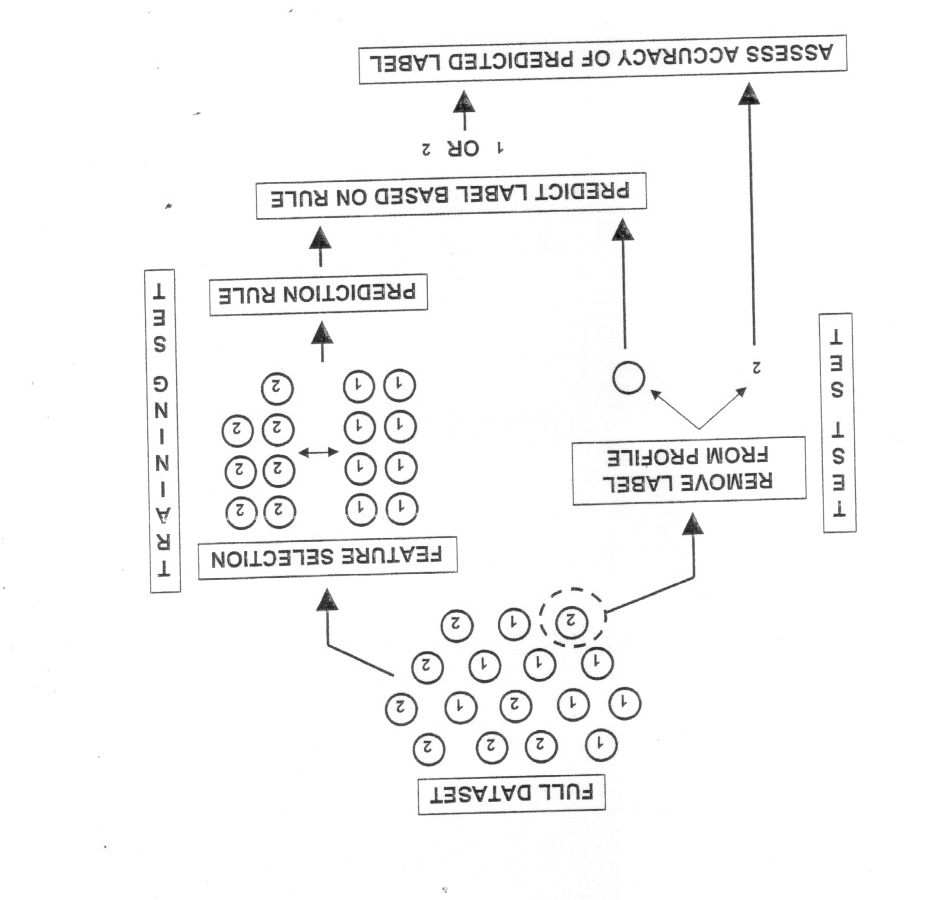
\includegraphics[scale=0.45,angle=178]{Figures/simon-cv.png}
  \end{figure}
\end{frame}




\begin{frame}[containsverbatim]
  \frametitle{Simulate Data for $k$-NN Prediction}
  \footnotesize
  \begin{itemize}
  \item Simulate expression from 1000 genes for 
        40 patients. Let the first 20 be responders
        and the remaining 20 be non-responders
\begin{knitrout}\tiny
\definecolor{shadecolor}{rgb}{0.969, 0.969, 0.969}\color{fgcolor}\begin{kframe}
\begin{alltt}
\hlkwd{set.seed}\hlstd{(}\hlnum{123}\hlstd{)}
\hlstd{n}\hlkwb{=}\hlnum{20}
\hlstd{m}\hlkwb{=}\hlnum{1000}
\hlstd{EXPRS}\hlkwb{=}\hlkwd{matrix}\hlstd{(}\hlkwd{rnorm}\hlstd{(}\hlnum{2}\hlopt{*}\hlstd{n}\hlopt{*}\hlstd{m),}\hlnum{2}\hlopt{*}\hlstd{n,m)}
\hlkwd{rownames}\hlstd{(EXPRS)}\hlkwb{=}\hlkwd{paste}\hlstd{(}\hlstr{"pt"}\hlstd{,}\hlnum{1}\hlopt{:}\hlstd{(}\hlnum{2}\hlopt{*}\hlstd{n),}\hlkwc{sep}\hlstd{=}\hlstr{""}\hlstd{)}
\hlkwd{colnames}\hlstd{(EXPRS)}\hlkwb{=}\hlkwd{paste}\hlstd{(}\hlstr{"g"}\hlstd{,}\hlnum{1}\hlopt{:}\hlstd{m,}\hlkwc{sep}\hlstd{=}\hlstr{""}\hlstd{)}
\hlstd{grp}\hlkwb{=}\hlkwd{rep}\hlstd{(}\hlnum{0}\hlopt{:}\hlnum{1}\hlstd{,}\hlkwd{c}\hlstd{(n,n))}
\end{alltt}
\end{kframe}
\end{knitrout}
\item Pick the top 10 features based on the 
  two-sample $t$-test
\begin{knitrout}\tiny
\definecolor{shadecolor}{rgb}{0.969, 0.969, 0.969}\color{fgcolor}\begin{kframe}
\begin{alltt}
\hlkwd{library}\hlstd{(genefilter)}
\hlstd{stats}\hlkwb{=}\hlkwd{abs}\hlstd{(}\hlkwd{rowttests}\hlstd{(}\hlkwd{t}\hlstd{(EXPRS),} \hlkwd{factor}\hlstd{(grp))}\hlopt{$}\hlstd{statistic)}
\hlstd{ii}\hlkwb{=}\hlkwd{order}\hlstd{(}\hlopt{-}\hlstd{stats)}
\end{alltt}
\end{kframe}
\end{knitrout}
\item Filter out all genes except the top 10
\begin{knitrout}\tiny
\definecolor{shadecolor}{rgb}{0.969, 0.969, 0.969}\color{fgcolor}\begin{kframe}
\begin{alltt}
\hlstd{TOPEXPRS}\hlkwb{=}\hlstd{EXPRS[, ii[}\hlnum{1}\hlopt{:}\hlnum{10}\hlstd{]]}
\end{alltt}
\end{kframe}
\end{knitrout}
  \end{itemize}
  
  
\end{frame}


\begin{frame}[containsverbatim]
  \frametitle{Error Resubstitution and Naive CV}
  \footnotesize
  \begin{itemize}
\item Error resubstitution (Training and Testing set are the same)
\begin{knitrout}\tiny
\definecolor{shadecolor}{rgb}{0.969, 0.969, 0.969}\color{fgcolor}\begin{kframe}
\begin{alltt}
\hlstd{mod0}\hlkwb{=}\hlkwd{knn}\hlstd{(}\hlkwc{train}\hlstd{=TOPEXPRS,}\hlkwc{test}\hlstd{=TOPEXPRS,}\hlkwc{cl}\hlstd{=grp,}\hlkwc{k}\hlstd{=}\hlnum{3}\hlstd{)}
\hlkwd{table}\hlstd{(mod0,grp)}
\end{alltt}
\begin{verbatim}
##     grp
## mod0  0  1
##    0 17  0
##    1  3 20
\end{verbatim}
\end{kframe}
\end{knitrout}
\item Cross-validated predictions (the features selection
      is not part of the CV process)
\begin{knitrout}\tiny
\definecolor{shadecolor}{rgb}{0.969, 0.969, 0.969}\color{fgcolor}\begin{kframe}
\begin{alltt}
\hlstd{mod1}\hlkwb{=}\hlkwd{knn.cv}\hlstd{(TOPEXPRS,grp,}\hlkwc{k}\hlstd{=}\hlnum{3}\hlstd{)}
\hlkwd{table}\hlstd{(mod1,grp)}
\end{alltt}
\begin{verbatim}
##     grp
## mod1  0  1
##    0 16  0
##    1  4 20
\end{verbatim}
\end{kframe}
\end{knitrout}
\item Note that in both examples, {\tt TOPEXPR} not {\tt EXPR}
  is used.
\end{itemize}
  
  
\end{frame}

\begin{frame}[containsverbatim]
  \frametitle{{\tt R} Function to Implement Proper CV based on $k$-NN}
\tiny
\begin{knitrout}\tiny
\definecolor{shadecolor}{rgb}{0.969, 0.969, 0.969}\color{fgcolor}\begin{kframe}
\begin{alltt}
\hlstd{top.features}\hlkwb{=}\hlkwa{function}\hlstd{(}\hlkwc{EXP}\hlstd{,}\hlkwc{resp}\hlstd{,}\hlkwc{test}\hlstd{,}\hlkwc{fsnum}\hlstd{)}
  \hlstd{\{}
    \hlstd{top.features.i}\hlkwb{=}\hlkwa{function}\hlstd{(}\hlkwc{i}\hlstd{,}\hlkwc{EXP}\hlstd{,}\hlkwc{resp}\hlstd{,}\hlkwc{test}\hlstd{,}\hlkwc{fsnum}\hlstd{)}
      \hlstd{\{}
        \hlstd{stats}\hlkwb{=}\hlkwd{abs}\hlstd{(}\hlkwd{mt.teststat}\hlstd{(EXP[,}\hlopt{-}\hlstd{i],resp[}\hlopt{-}\hlstd{i],}\hlkwc{test}\hlstd{=test))}
        \hlstd{ii}\hlkwb{=}\hlkwd{order}\hlstd{(}\hlopt{-}\hlstd{stats)[}\hlnum{1}\hlopt{:}\hlstd{fsnum]}
        \hlkwd{rownames}\hlstd{(EXP)[ii]}
      \hlstd{\}}
    \hlkwd{sapply}\hlstd{(}\hlnum{1}\hlopt{:}\hlkwd{ncol}\hlstd{(EXP),top.features.i,}\hlkwc{EXP}\hlstd{=EXP,}\hlkwc{resp}\hlstd{=resp,}\hlkwc{test}\hlstd{=test,}\hlkwc{fsnum}\hlstd{=fsnum)}
  \hlstd{\}}


\hlcom{# This function evaluates the knn}

\hlstd{knn.loocv}\hlkwb{=}\hlkwa{function}\hlstd{(}\hlkwc{EXP}\hlstd{,}\hlkwc{resp}\hlstd{,}\hlkwc{test}\hlstd{,}\hlkwc{k}\hlstd{,}\hlkwc{fsnum}\hlstd{,}\hlkwc{tabulate}\hlstd{=}\hlnum{FALSE}\hlstd{,}\hlkwc{permute}\hlstd{=}\hlnum{FALSE}\hlstd{)}
  \hlstd{\{}
    \hlkwa{if}\hlstd{(permute)}
      \hlstd{resp}\hlkwb{=}\hlkwd{sample}\hlstd{(resp)}
    \hlstd{topfeat}\hlkwb{=}\hlkwd{top.features}\hlstd{(EXP,resp,test,fsnum)}
    \hlstd{pids}\hlkwb{=}\hlkwd{rownames}\hlstd{(EXP)}
    \hlstd{EXP}\hlkwb{=}\hlkwd{t}\hlstd{(EXP)}
    \hlkwd{colnames}\hlstd{(EXP)}\hlkwb{=}\hlkwd{as.character}\hlstd{(pids)}
    \hlstd{knn.loocv.i}\hlkwb{=}\hlkwa{function}\hlstd{(}\hlkwc{i}\hlstd{,}\hlkwc{EXP}\hlstd{,}\hlkwc{resp}\hlstd{,}\hlkwc{k}\hlstd{,}\hlkwc{topfeat}\hlstd{)}
      \hlstd{\{}
        \hlstd{ii}\hlkwb{=}\hlstd{topfeat[,i]}
        \hlstd{mod}\hlkwb{=}\hlkwd{knn}\hlstd{(}\hlkwc{train}\hlstd{=EXP[}\hlopt{-}\hlstd{i,ii],}\hlkwc{test}\hlstd{=EXP[i,ii],}\hlkwc{cl}\hlstd{=resp[}\hlopt{-}\hlstd{i],}\hlkwc{k}\hlstd{=k)[}\hlnum{1}\hlstd{]}
      \hlstd{\}}
    \hlstd{out}\hlkwb{=}\hlkwd{sapply}\hlstd{(}\hlnum{1}\hlopt{:}\hlkwd{nrow}\hlstd{(EXP),knn.loocv.i,}\hlkwc{EXP}\hlstd{=EXP,}\hlkwc{resp}\hlstd{=resp,}\hlkwc{k}\hlstd{=k,}\hlkwc{topfeat}\hlstd{=topfeat)}
    \hlkwa{if}\hlstd{(tabulate)}
      \hlstd{out}\hlkwb{=}\hlkwd{ftable}\hlstd{(}\hlkwc{pred}\hlstd{=out,}\hlkwc{obs}\hlstd{=resp)}
    \hlkwd{return}\hlstd{(out)}
  \hlstd{\}}
\end{alltt}
\end{kframe}
\end{knitrout}
\end{frame}


\begin{frame}[containsverbatim]
  \frametitle{Proper Cross-Validation}
  \footnotesize
  \begin{itemize}
  \item Finally, we conduct proper cross-validation using the 
        previous {\tt R} function
  \item At each iteration, the top 10 features are selected
        based on the data from the $n-1$ samples in the training set
\begin{knitrout}\tiny
\definecolor{shadecolor}{rgb}{0.969, 0.969, 0.969}\color{fgcolor}\begin{kframe}
\begin{alltt}
\hlkwd{knn.loocv}\hlstd{(}\hlkwd{t}\hlstd{(EXPRS),}\hlkwd{as.integer}\hlstd{(grp),}\hlstr{"t.equalvar"}\hlstd{,}\hlnum{3}\hlstd{,}\hlnum{10}\hlstd{,}\hlnum{TRUE}\hlstd{)}
\end{alltt}
\begin{verbatim}
##      obs  0  1
## pred          
## 0         7  7
## 1        13 13
\end{verbatim}
\end{kframe}
\end{knitrout}
\item Note that {\tt EXPRS} not {\tt TOPEXPR} is used.
\item The classification rate is 50\% (as expected)
\end{itemize}
  
\end{frame}


\begin{frame}{Naive LOOCV: Quantitative trait}
  \begin{itemize}
  \item Repeat the last experiment with a noisy quantitative outcome
  \item First simulate a data matrix of dimension $n=50$ (patients) and $m$ (genes)
  \item Next draw the outcome for $n=50$ patients from a standard
        normal distribution independent of the data matrix
  \item There is no relationship between the expressions and the outcome (by design)
  \item We consider $m=45$ and $m=50000$
  \item We conduct Naive LOOCV using the top 10 features 
  \end{itemize}
\end{frame}

\begin{frame}{Naive LOOCV: Quantitative trait}
  \begin{figure}
    \centering
    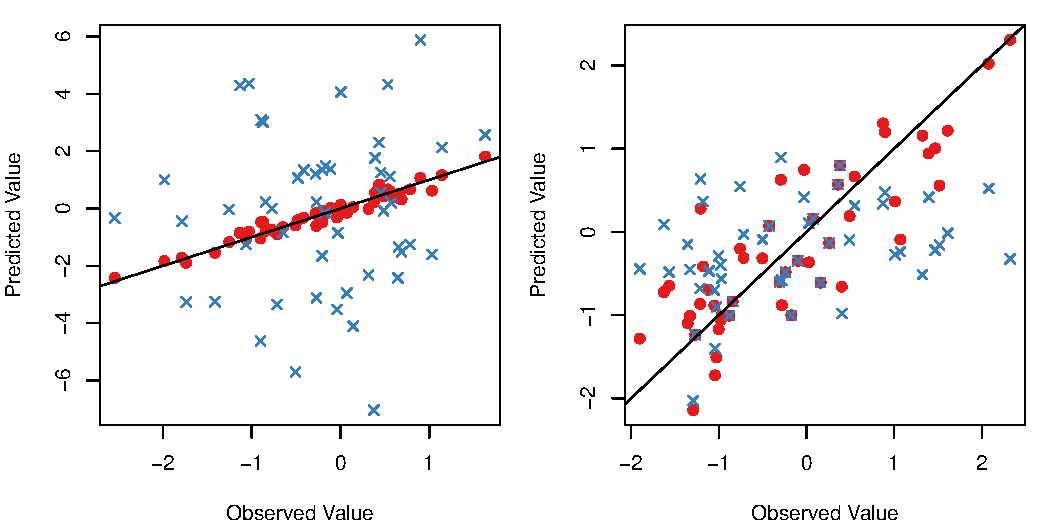
\includegraphics[scale=0.65]{Figures/lm-overfit.pdf}
  \end{figure}
Figure taken from Owzar {\it et al}; {\it Clin Transl Sci} 2011. 
\end{frame}


\begin{frame}
  \frametitle{Training, Validation and Testing Approach}
  \begin{itemize}
  \item Before you test the model, you must freeze it
  \item You may want to split the Training set further into
        a Training and Validation set
  \item Use the Validation set to "tune" the model.
  \end{itemize}
\end{frame}

\begin{frame}
  \frametitle{Final Remarks}
  \begin{itemize}
  \item It is OK to try different methods (other classifiers, feature selection or tuning methods)
  \item Keep track of what you have done and report it (brief description in the paper and details in 
        supplementary material)
  \item Be careful if you have too few responders
  \item You could have a model that will classify most patients as a non-responder.
  \item In this case a 00 ($Y=0$ and $g(X)=0$) may not be bona-fide true-negative
  \item The gold-standard for model validation, is to follow up the cross-validatiion by permutation resampling
    \item The {\tt R} function provided can be used for this purpose
\end{itemize}
\end{frame}



%% \begin{frame}
%%   \frametitle{Pre-processing Challenge}
%%   \begin{itemize}
%%   \item The expressions from the testing set need to be "compatible" to those used to
%%         train the model
%%   \item In classical experiments with a few biomarkers, the labs had internal controls
%%         to ensure that the measurements were properly normalized
%%   \item This is very complicated in microarray experiments (it is hard enough to do this for a single batch let alone for two batches)
%%   \item If the model is used to stratify patients into a clinical study, then one has to be extra careful (due to ethical issues)
%%   \item This problem has (our opinion) not been addressed appropriately 
%%          in the literature.
%%   \item Microarray assays provide {\it relative} not {\tt absolute} expressions
%%   \end{itemize}
%% \end{frame}
%% \begin{frame}
%%   \frametitle{Director's Challenge Lung Cancer Data (Shedden et al)}
%% \setkeys{Gin}{width=0.7\textwidth}

%%   \begin{figure}
%%    \centering
%%    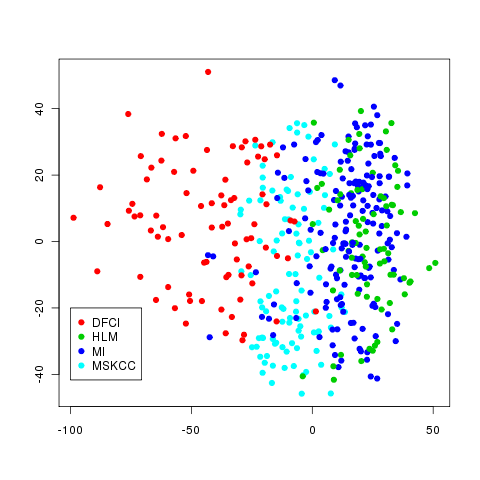
\includegraphics[scale=0.5]{Figures/dchallenge-batch.png}
%%  \end{figure}
%% \end{frame}

%% \begin{frame}
%%   \frametitle{On Data and Answers}
%% "The data may not contain the answer. The combination of 
%% some data and an aching desire for an answer does not ensure 
%% that a reasonable answer can be extracted from a given body of data."
%% \vskip 0.5in
%% John Wilder Tukey

%% \end{frame}
\section[Class Discovery]{Elements of Unsupervised Learning}

\begin{frame}
  \frametitle{Scope}
  \begin{itemize}
\item Often we would like to discover clusters or outliers based on the
      gene expression profiles
\item These are {\it unsupervised} methods in the sense that the algorithm
      knows nothing about the outcome 
\item It is only aware of the gene profiles
  ($X$) and not the outcome $Y$
\end{itemize}
\end{frame}

\begin{frame}{Fisher's Iris Data}
\begin{knitrout}\tiny
\definecolor{shadecolor}{rgb}{0.969, 0.969, 0.969}\color{fgcolor}

{\centering 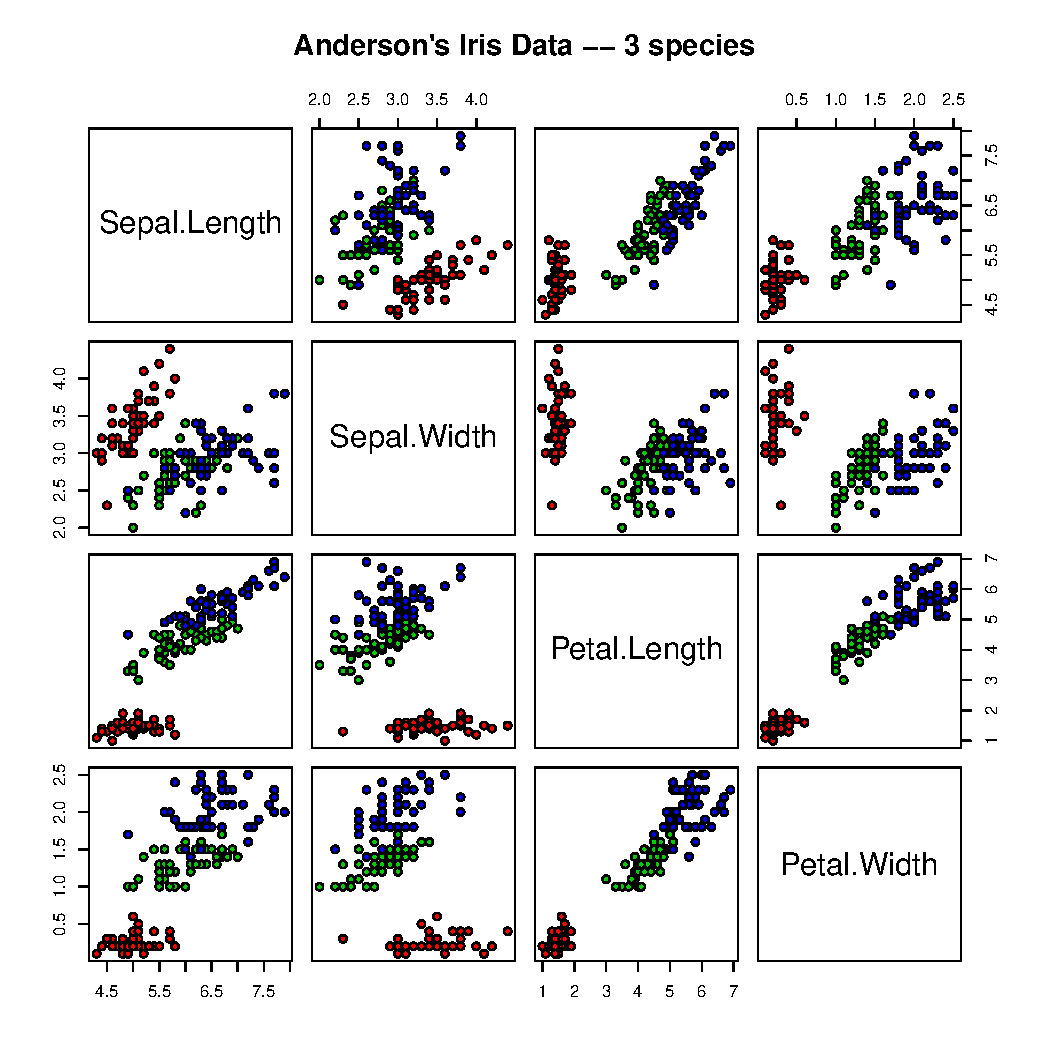
\includegraphics[width=.6\linewidth]{figure/beamer-iris1-1} 

}



\end{knitrout}
\end{frame}


\begin{frame}{Fisher's Iris Data}
\begin{knitrout}\tiny
\definecolor{shadecolor}{rgb}{0.969, 0.969, 0.969}\color{fgcolor}

{\centering 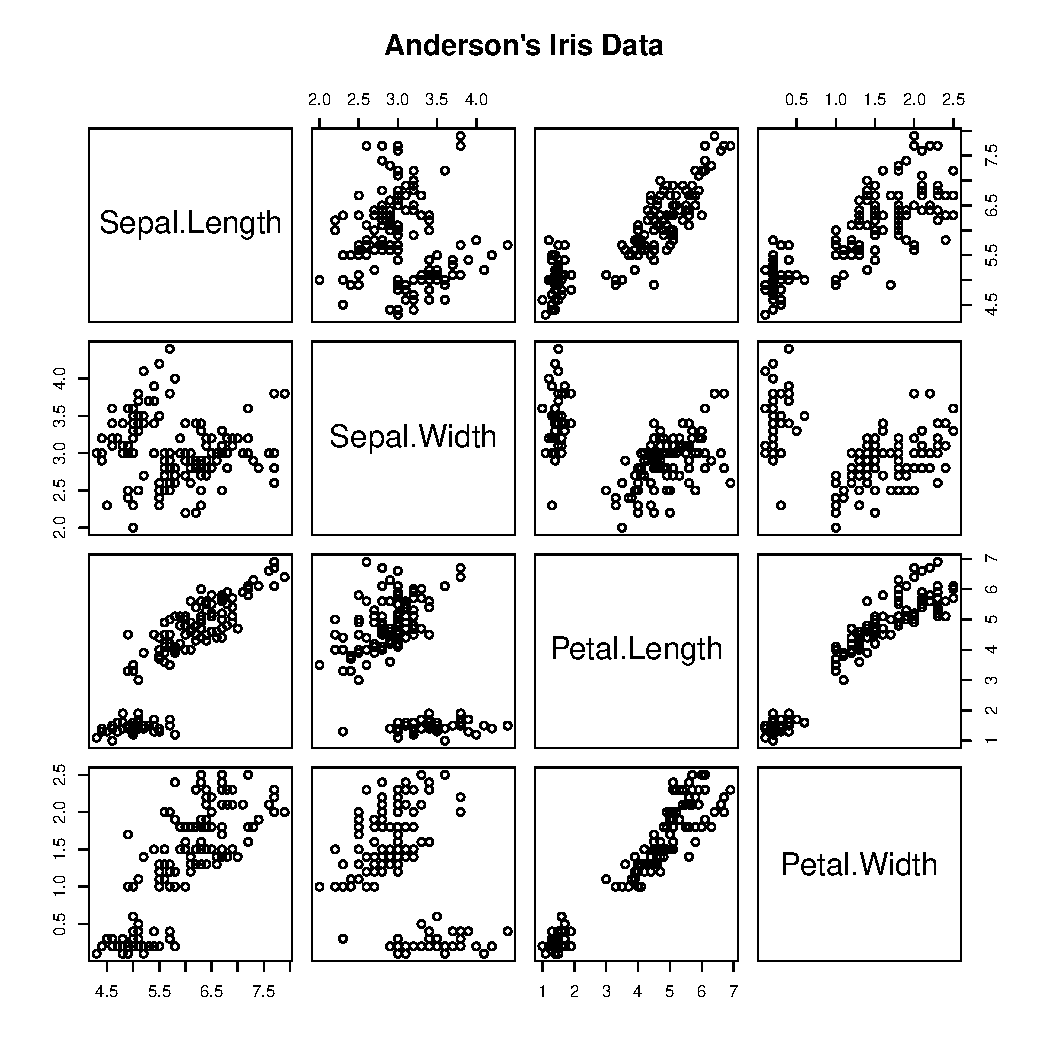
\includegraphics[width=.6\linewidth]{figure/beamer-iris2-1} 

}



\end{knitrout}
\end{frame}


\begin{frame}{A Self-fulfilling Prophecy}
  \begin{itemize}
  \item Statistical method for unsupervised learning guarantee one thing
  \item They will return a clustering of your data
  \item What they do not guarantee and are invariably unable to 
        verify, is the biological relevance or reproducibility of the clustering
  \item In light of this Self-fulfilling Prophecy, these methods should be used
      with utmost care
  \end{itemize}
\end{frame}


\begin{frame}{Golub {\it et al} Leukemia Data}
  \begin{itemize}
  \item 47 patients with acute lymphoblastic leukemia (ALL) 
  \item 25 patients with acute myeloid leukemia (AML)
  \item Platform: Affymetrix Hgu6800
  \item 7129 probe sets
  \item Golub {\it et al.} (1999). Molecular classification of cancer: class discovery and class prediction by gene expression monitoring, Science, Vol. 286:531-537.
  \end{itemize}
\end{frame}

\begin{frame}{ Chiaretti {\it et al} ALL Data}
  \begin{itemize}
  \item 128 patients with acute lymphoblastic leukemia (ALL) 
  \item Platform: Affymetrix hgu95av2
  \item 12625 probe sets
  \item  Chiaretti {\it et al.} 
     Gene
     expression profile of adult T-cell acute lymphocytic leukemia
     identifies distinct subsets of patients with different response to
     therapy and survival. {\it Blood}, 1 April 2004, Vol. 103, No. 7.
  \end{itemize}
\end{frame}

\begin{frame}
  \frametitle{Methods to be Discussed}
  \begin{itemize}
\item There are many methods for unsupervised class 
      discovery.
\item We will consider three types of methods:
  \begin{itemize}
  \item Ordination Methods (e.g., Multi-Dimensional Scaling (MDS) and Principal Components (PC))
  \item Hierarchical Clustering
  \item $k$-means Clustering
  \end{itemize}
\item Note that there are many variations of these methods
\item Most mathematical details will be left out
\item We focus on discovering classes among patients (not genes)
\end{itemize}
\end{frame}


\begin{frame}
  \frametitle{Distance between Two Points}
  \begin{itemize}
\item Many class discover methods aim to quantify the similarity
      (or dissimilarity) among patients
\item For each patient, the vector of gene expression can be thought
      of a "point" in a $m$-dimensional space
\item For many class discovery methods, one has to be able to quantify
      the "distance" between two points (the expression profiles
      between two individuals)
\item A common distance measure is the Euclidean distance
\end{itemize}

\end{frame}


\begin{frame}[plain]
  \frametitle{Distance (Two points on the plane)}
\begin{figure}
  \centering  
\begin{knitrout}\tiny
\definecolor{shadecolor}{rgb}{0.969, 0.969, 0.969}\color{fgcolor}

{\centering 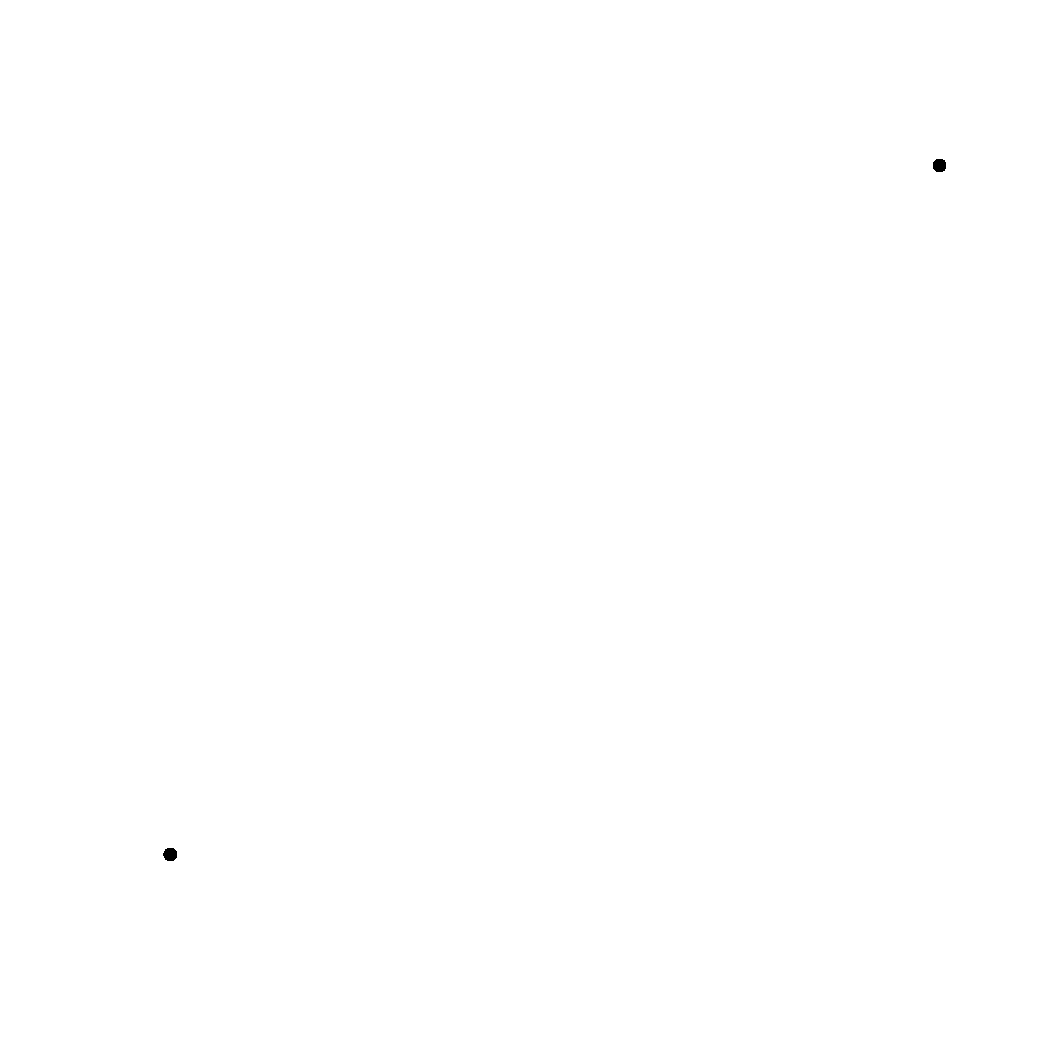
\includegraphics[width=.6\linewidth]{figure/beamer-dist1-1} 

}



\end{knitrout}
\end{figure}
\end{frame}


\begin{frame}[plain]
  \frametitle{Distance (Coordinates)}

\begin{knitrout}\tiny
\definecolor{shadecolor}{rgb}{0.969, 0.969, 0.969}\color{fgcolor}

{\centering 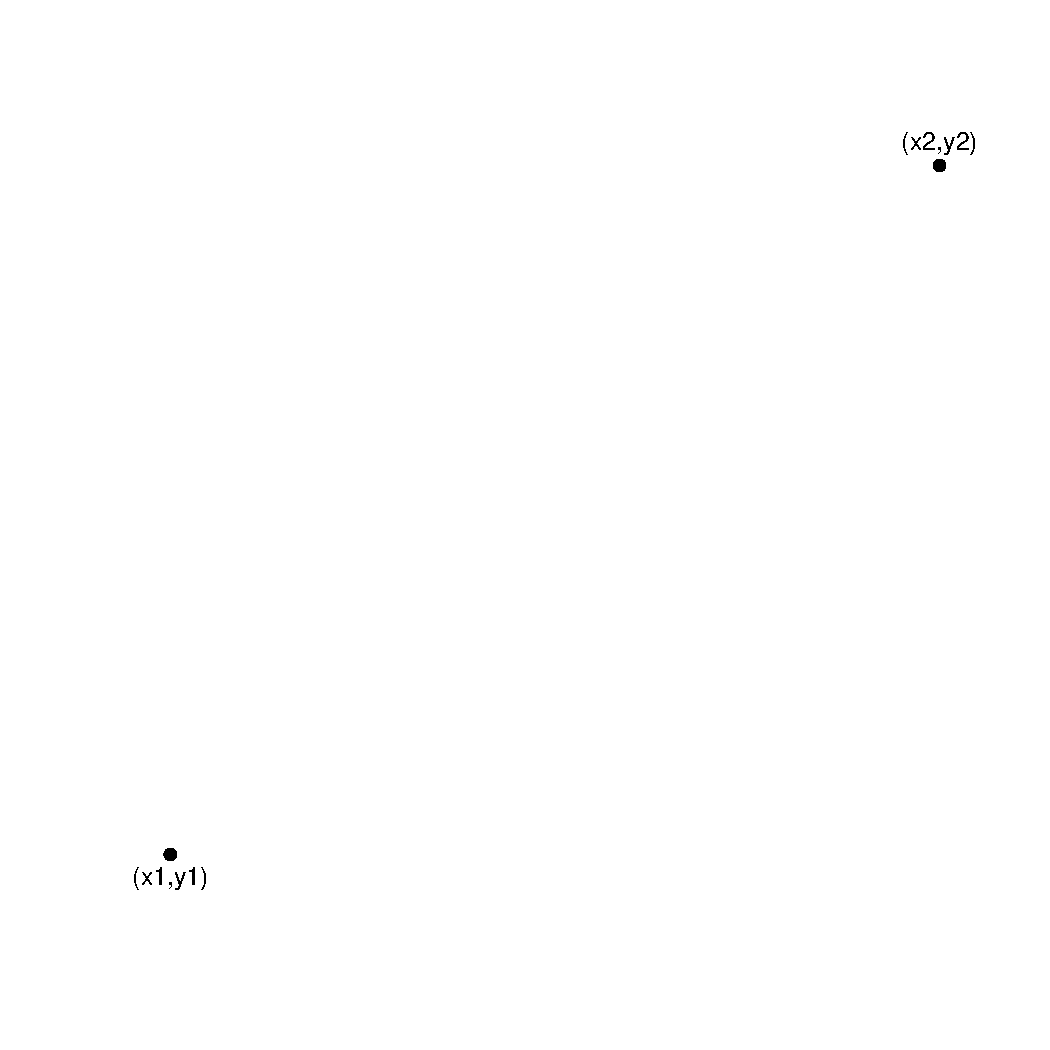
\includegraphics[width=.6\linewidth]{figure/beamer-dist2-1} 

}



\end{knitrout}

\end{frame}


\begin{frame}[plain]
  \frametitle{Distance}

\begin{knitrout}\tiny
\definecolor{shadecolor}{rgb}{0.969, 0.969, 0.969}\color{fgcolor}

{\centering 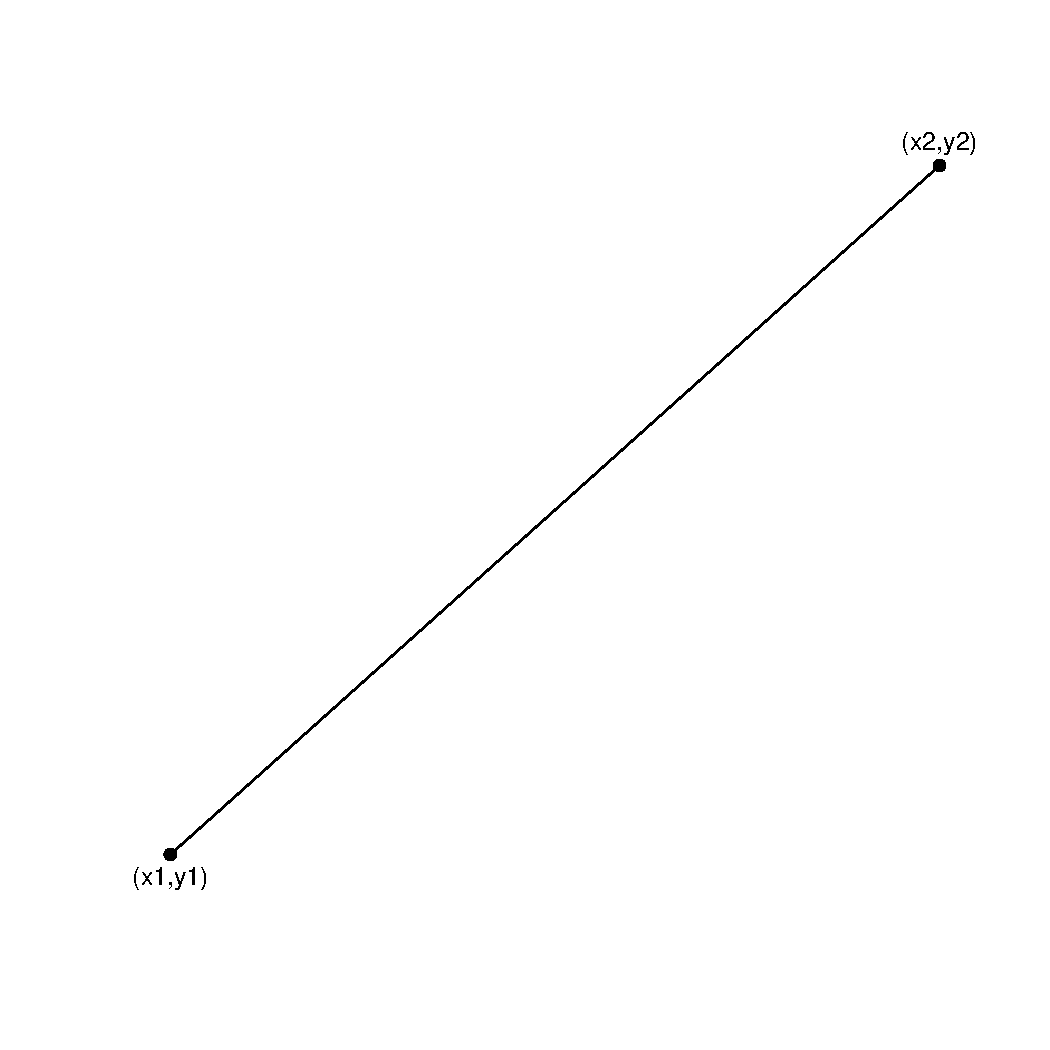
\includegraphics[width=.6\linewidth]{figure/beamer-dist3-1} 

}



\end{knitrout}

\end{frame}

\begin{frame}[plain]
  \frametitle{Distance (horizontal/vertical shifts)}
\begin{knitrout}\tiny
\definecolor{shadecolor}{rgb}{0.969, 0.969, 0.969}\color{fgcolor}

{\centering 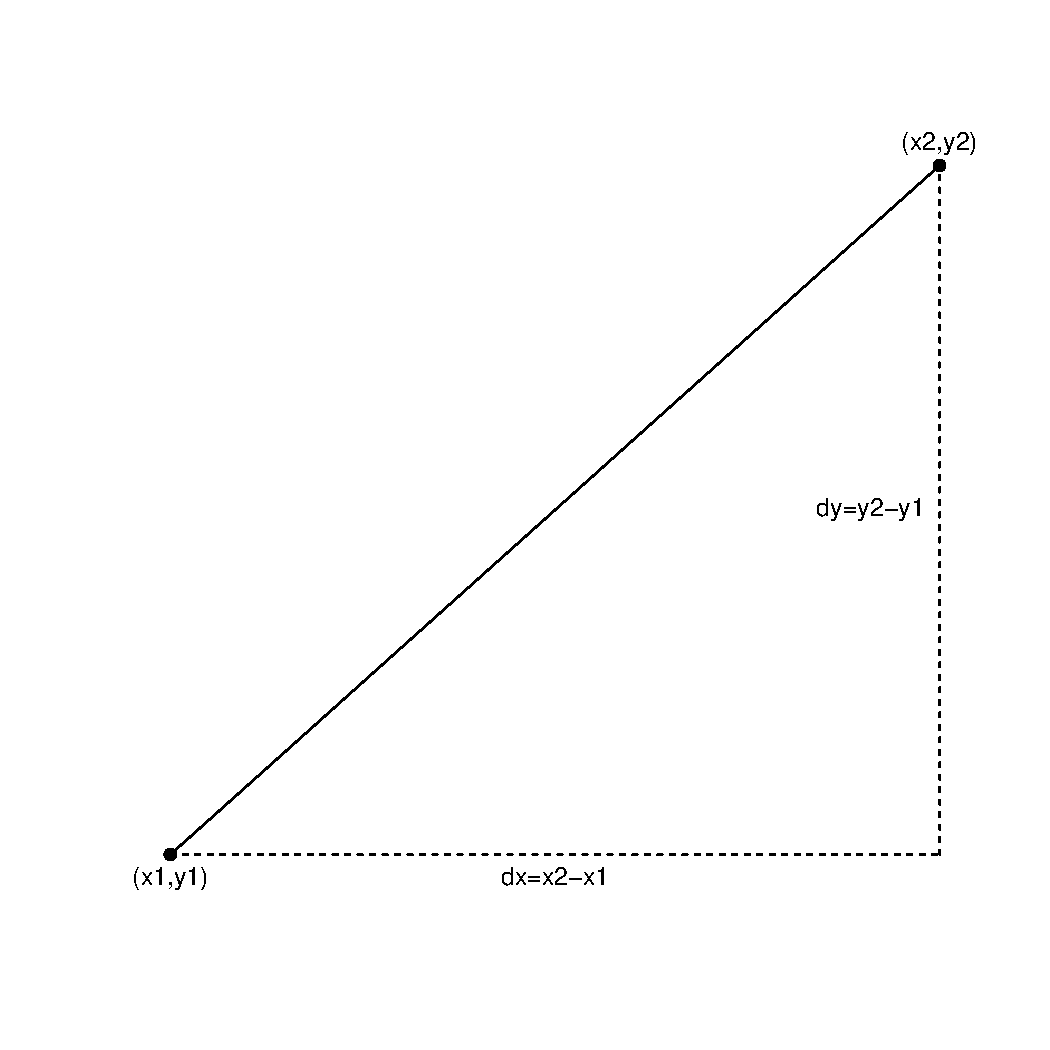
\includegraphics[width=.6\linewidth]{figure/beamer-dist4-1} 

}



\end{knitrout}
\end{frame}


\begin{frame}{Relative Distance (From CST 2011 Paper)}
  
  \begin{figure}
   \centering
   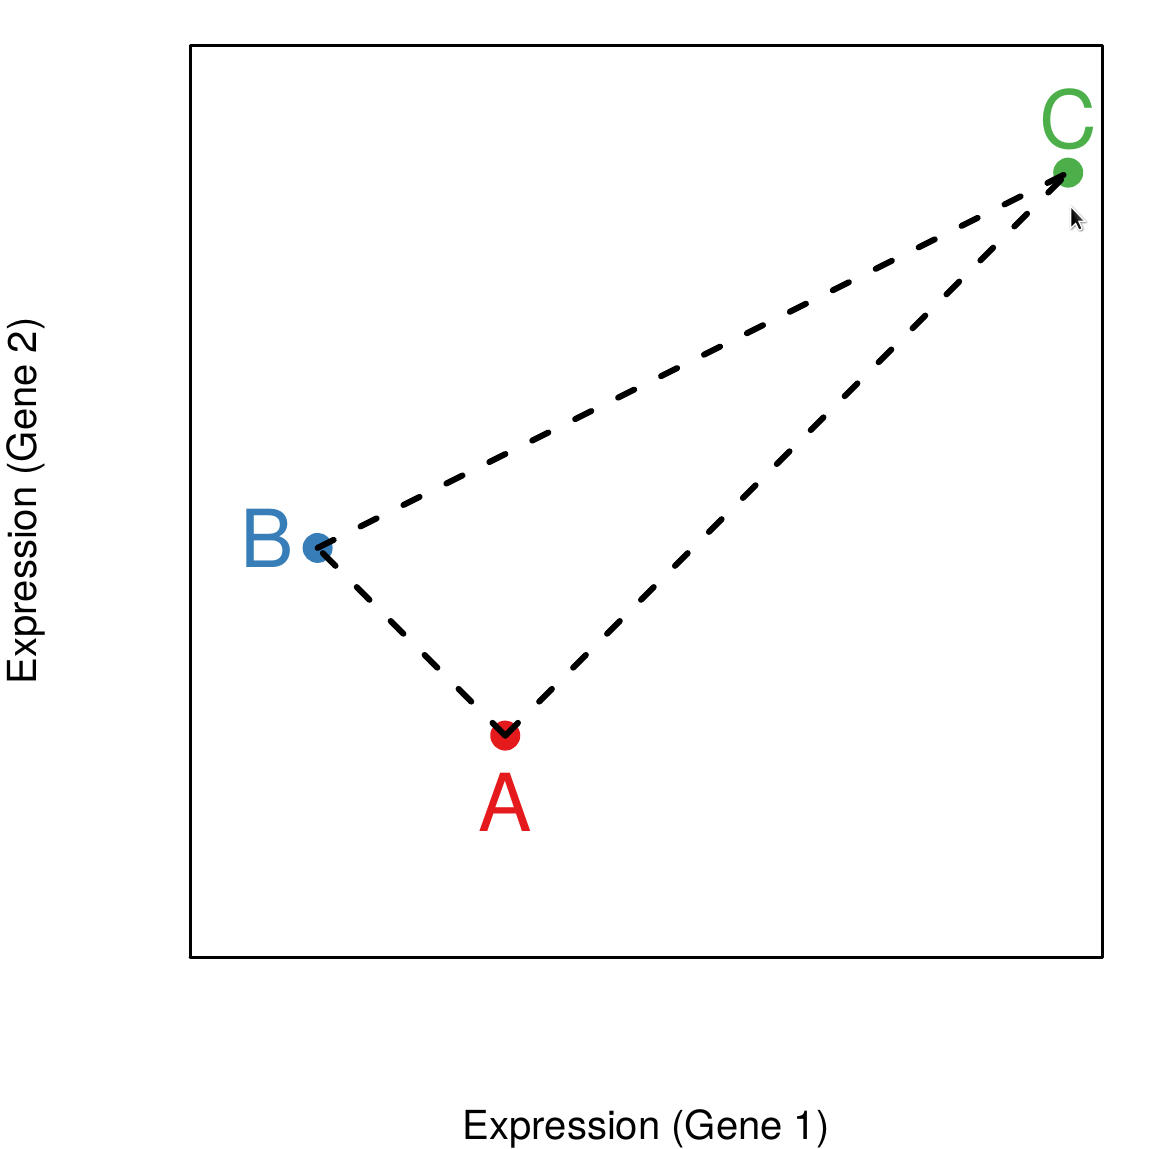
\includegraphics[scale=0.4]{Figures/distance.png}
 \end{figure}
\end{frame}


%% \begin{frame}
%%   \frametitle{Pythagorean Theorem (on the plane)}
%% \begin{itemize}
%% \item According to the Pythagorean theorem
%% $$
%% h^2=\mathrm{d}x^2+\mathrm{d}y^2=(x_2-x_1)^2+(y_2-y_1)^2
%% $$
%% \item $h$ is called the hypotenuse
%% \item The distance between $(x_1,y_1)$ and $(x_2,y_2)$ is given by
%% $$
%% h=\sqrt{\mathrm{d}x^2+\mathrm{d}y^2}=\sqrt{(x_2-x_1)^2+(y_2-y_1)^2}
%% $$

%% \end{itemize}
 
%% \end{frame}

%% \begin{frame}
%%   \frametitle{Pythagorean Theorem (on the plane)}
%% \begin{itemize}
%% \item Can be extended to higher dimensions
%% \item In a three-dimensional space the distance between
%%   $(x_1,y_1,z_1)$ and $(x_2,y_2,z_2)$ is given by 
%% $$
%% \sqrt{(x_1-x_2)^2+(y_1-y_2)^2+(z_1-z_2)^2}
%% $$
%% \item For any given dimension, the distance is obtained as the square root
%%       of the sum of the 
%%       square of the coordinate-wise differences 
%% \end{itemize}

%% \end{frame}

%% \begin{frame}
%%   \frametitle{Euclidean Space}
%% \begin{itemize}
%% \item The line, plane and so called 3d space are Euclidean spaces of dimensions 1,2 and 3
%%       respectively
%% \item A Euclidean space of dimension $d$ is typically denoted by $\mathbb R^d$
%% \item The distance measure we discussed is called the Euclidean distance
%% \item There are many other types of distances
%% \item Think of each patient as a point in the $\mathbb R^m$ space where $m$ is the number of probe sets
%% \item Use a distance to quantify similarity (or dissimilarity) among patients
%% \item A "small" distance suggests that two patients are "similar"
%% \end{itemize}
%% \end{frame}

\begin{frame}[fragile]{Dissimilarity matrix}
  \begin{itemize}
  \item Use a distance to quantify similarity (or dissimilarity) among patients
  \item A matrix containing all pairwise distances
  \item Take the first three patients in the Golub data set (based on
    7129 probe sets
\begin{knitrout}\tiny
\definecolor{shadecolor}{rgb}{0.969, 0.969, 0.969}\color{fgcolor}\begin{kframe}
\begin{alltt}
\hlkwd{dist}\hlstd{(}\hlkwd{t}\hlstd{(}\hlkwd{exprs}\hlstd{(Golub_Merge[,}\hlnum{1}\hlopt{:}\hlnum{3}\hlstd{])))}
\end{alltt}
\begin{verbatim}
##           39        40
## 40 101530.75          
## 42  94405.04  89502.29
\end{verbatim}
\end{kframe}
\end{knitrout}
\item The distance between patient 39 and 40 is 
  \ensuremath{1.0153075\times 10^{5}}
\item Let us calculate this by hand
\begin{knitrout}\tiny
\definecolor{shadecolor}{rgb}{0.969, 0.969, 0.969}\color{fgcolor}\begin{kframe}
\begin{alltt}
\hlstd{x}\hlkwb{=}\hlkwd{exprs}\hlstd{(Golub_Merge)[,}\hlstr{"39"}\hlstd{]}
\hlstd{y}\hlkwb{=}\hlkwd{exprs}\hlstd{(Golub_Merge)[,}\hlstr{"40"}\hlstd{]}
\hlkwd{sqrt}\hlstd{(}\hlkwd{sum}\hlstd{((x}\hlopt{-}\hlstd{y)}\hlopt{^}\hlnum{2}\hlstd{))}
\end{alltt}
\begin{verbatim}
## [1] 101530.8
\end{verbatim}
\end{kframe}
\end{knitrout}
\end{itemize}
\end{frame}


\begin{frame}
  \frametitle{Dimension reduction}
  \begin{itemize}
\item Genome-wide profiling platforms are high-dimensional ($m$ is large)
\item Visualization beyond $m=3$ not possible (for mortals)
\item Representing the data by a lower dimensional format without losing
      too much information is desired.
\end{itemize}
\end{frame}





\begin{frame}
  \frametitle{Multi-Dimensional Scaling (MDS)}
  \begin{itemize}
\item Compute the dissimilarity matrix based on a distance measure
\item Project the points into a lower dimensional space (say 2D or 3D) 
      while preserving the similarity matrix
\item PCA is a related (and in a sense equivalent method to MDS)
\item Project the points into a lower dimensional space where the new variables
      are linear combinations of the original variables
\item The new variables are chosen so as to have maximum variance and to be uncorrelated.
\end{itemize}
\end{frame}






\begin{frame}[containsverbatim]
  \frametitle{MDS for Golub Data}
\begin{knitrout}\tiny
\definecolor{shadecolor}{rgb}{0.969, 0.969, 0.969}\color{fgcolor}

{\centering 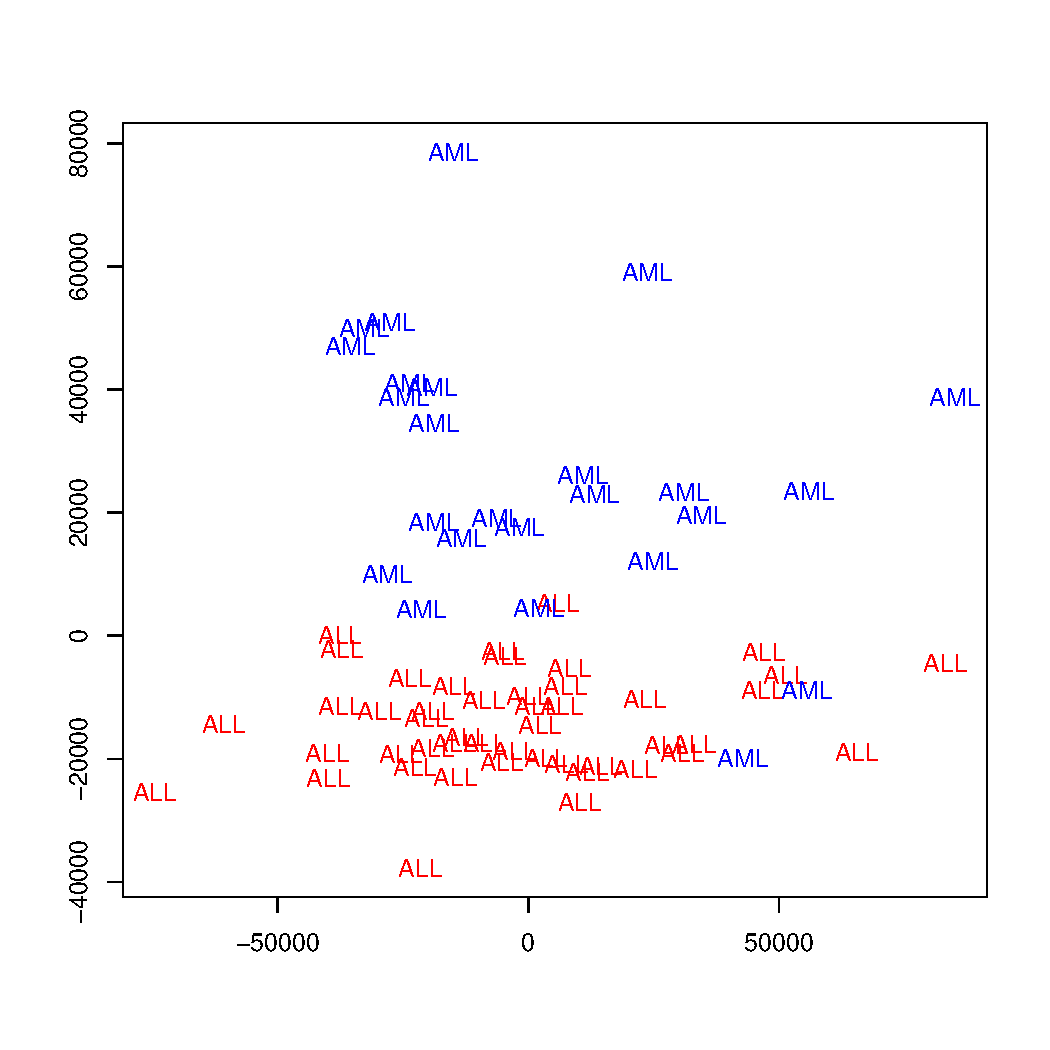
\includegraphics[width=.6\linewidth]{figure/beamer-mdsgolub-1} 

}



\end{knitrout}
\end{frame}

\begin{frame}[containsverbatim]
  \frametitle{PCA for Golub Data}
\begin{knitrout}\tiny
\definecolor{shadecolor}{rgb}{0.969, 0.969, 0.969}\color{fgcolor}

{\centering 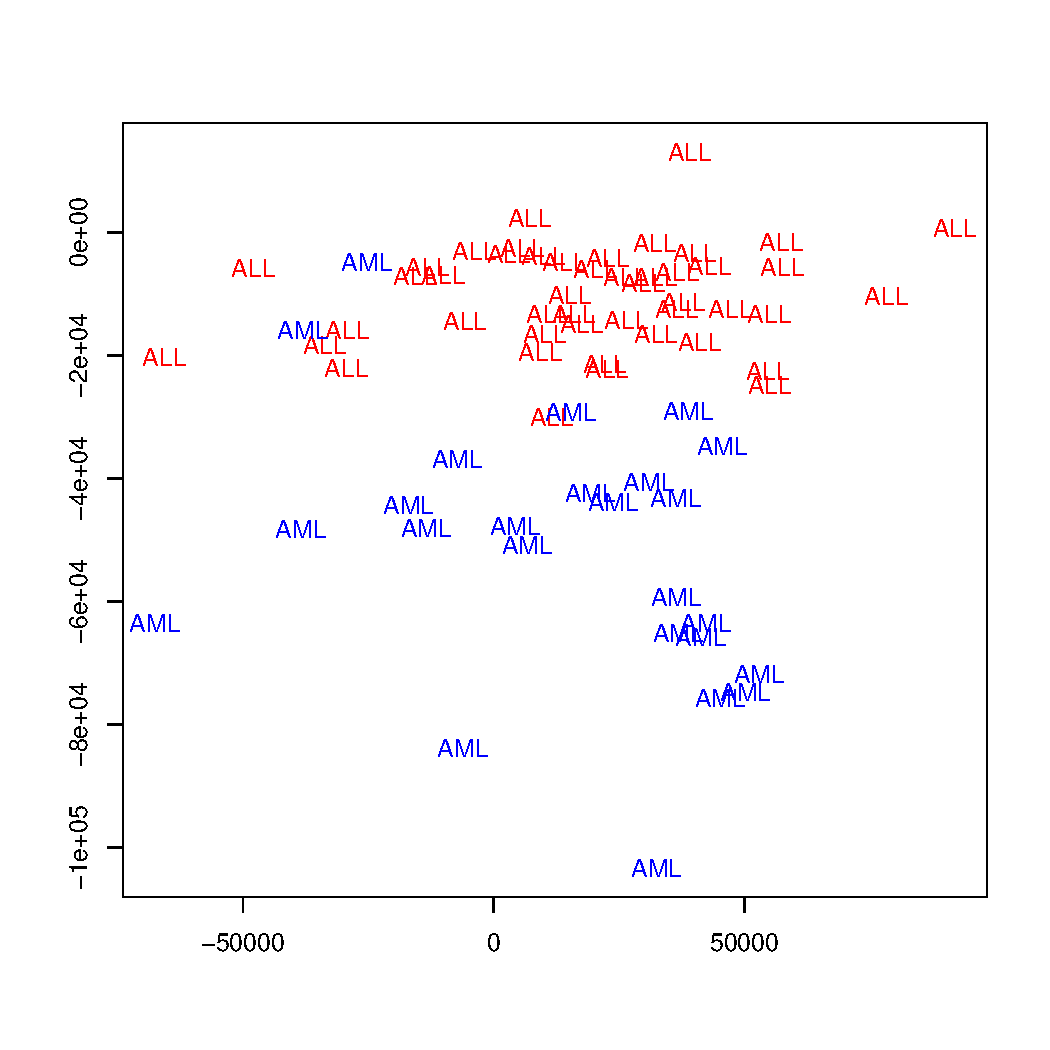
\includegraphics[width=.6\linewidth]{figure/beamer-pcagolub-1} 

}



\end{knitrout}
\end{frame}

\begin{frame}[containsverbatim]
  \frametitle{Preserving The Distances}
\footnotesize
  \begin{itemize}
\item Extract and standardize expression matrix for Golub data set
\begin{knitrout}\tiny
\definecolor{shadecolor}{rgb}{0.969, 0.969, 0.969}\color{fgcolor}\begin{kframe}
\begin{alltt}
\hlstd{scexpdat}\hlkwb{=}\hlkwd{scale}\hlstd{(}\hlkwd{t}\hlstd{(}\hlkwd{exprs}\hlstd{(Golub_Merge)))}
\hlkwd{dim}\hlstd{(scexpdat)}
\end{alltt}
\begin{verbatim}
## [1]   72 7129
\end{verbatim}
\end{kframe}
\end{knitrout}
\item Check means for the first 4 genes
\begin{knitrout}\tiny
\definecolor{shadecolor}{rgb}{0.969, 0.969, 0.969}\color{fgcolor}\begin{kframe}
\begin{alltt}
\hlkwd{apply}\hlstd{(scexpdat[,}\hlnum{1}\hlopt{:}\hlnum{4}\hlstd{],}\hlnum{2}\hlstd{,mean)}
\end{alltt}
\begin{verbatim}
## AFFX-BioB-5_at AFFX-BioB-M_at AFFX-BioB-3_at AFFX-BioC-5_at 
##  -7.841417e-17  -4.460287e-18   1.491832e-17  -5.051177e-17
\end{verbatim}
\end{kframe}
\end{knitrout}
\item Check standard deviations for the first 4 genes
\begin{knitrout}\tiny
\definecolor{shadecolor}{rgb}{0.969, 0.969, 0.969}\color{fgcolor}\begin{kframe}
\begin{alltt}
\hlkwd{apply}\hlstd{(scexpdat[,}\hlnum{1}\hlopt{:}\hlnum{4}\hlstd{],}\hlnum{2}\hlstd{,sd)}
\end{alltt}
\begin{verbatim}
## AFFX-BioB-5_at AFFX-BioB-M_at AFFX-BioB-3_at AFFX-BioC-5_at 
##              1              1              1              1
\end{verbatim}
\end{kframe}
\end{knitrout}
\end{itemize}
\end{frame}

\begin{frame}[containsverbatim]
  \frametitle{Preserving The Distances}
\footnotesize
  \begin{itemize}
\item Check distance among the first three patients
\begin{knitrout}\tiny
\definecolor{shadecolor}{rgb}{0.969, 0.969, 0.969}\color{fgcolor}\begin{kframe}
\begin{alltt}
\hlkwd{dist}\hlstd{(scexpdat[}\hlnum{1}\hlopt{:}\hlnum{3}\hlstd{,])}
\end{alltt}
\begin{verbatim}
##          39       40
## 40 125.3402         
## 42 118.1911 125.0390
\end{verbatim}
\end{kframe}
\end{knitrout}
\item Calculate MDS $d=2$
\begin{knitrout}\tiny
\definecolor{shadecolor}{rgb}{0.969, 0.969, 0.969}\color{fgcolor}\begin{kframe}
\begin{alltt}
\hlstd{MDS}\hlkwb{=}\hlkwd{cmdscale}\hlstd{(}\hlkwd{dist}\hlstd{(scexpdat),}\hlnum{2}\hlstd{)}
\hlkwd{dist}\hlstd{(MDS[}\hlnum{1}\hlopt{:}\hlnum{3}\hlstd{,])}
\end{alltt}
\begin{verbatim}
##           39        40
## 40  4.644939          
## 42 29.665656 34.287630
\end{verbatim}
\end{kframe}
\end{knitrout}
\item Calculate MDS $d=3$
\begin{knitrout}\tiny
\definecolor{shadecolor}{rgb}{0.969, 0.969, 0.969}\color{fgcolor}\begin{kframe}
\begin{alltt}
\hlstd{MDS}\hlkwb{=}\hlkwd{cmdscale}\hlstd{(}\hlkwd{dist}\hlstd{(scexpdat),}\hlnum{3}\hlstd{)}
\hlkwd{dist}\hlstd{(MDS[}\hlnum{1}\hlopt{:}\hlnum{3}\hlstd{,])}
\end{alltt}
\begin{verbatim}
##           39        40
## 40  9.293559          
## 42 45.719192 54.869668
\end{verbatim}
\end{kframe}
\end{knitrout}

  \end{itemize}
\end{frame}
\begin{frame}[containsverbatim]
  \frametitle{Preserving The Distances}
\footnotesize
  \begin{itemize}
\item Check distance among the first three patients
\begin{knitrout}\tiny
\definecolor{shadecolor}{rgb}{0.969, 0.969, 0.969}\color{fgcolor}\begin{kframe}
\begin{alltt}
\hlkwd{dist}\hlstd{(scexpdat[}\hlnum{1}\hlopt{:}\hlnum{3}\hlstd{,])}
\end{alltt}
\begin{verbatim}
##          39       40
## 40 125.3402         
## 42 118.1911 125.0390
\end{verbatim}
\end{kframe}
\end{knitrout}
\item Calculate MDS $d=20$
\begin{knitrout}\tiny
\definecolor{shadecolor}{rgb}{0.969, 0.969, 0.969}\color{fgcolor}\begin{kframe}
\begin{alltt}
\hlstd{MDS}\hlkwb{=}\hlkwd{cmdscale}\hlstd{(}\hlkwd{dist}\hlstd{(scexpdat),}\hlnum{3}\hlstd{)}
\hlkwd{dist}\hlstd{(MDS[}\hlnum{1}\hlopt{:}\hlnum{3}\hlstd{,])}
\end{alltt}
\begin{verbatim}
##           39        40
## 40  9.293559          
## 42 45.719192 54.869668
\end{verbatim}
\end{kframe}
\end{knitrout}
\item Calculate MDS $d=45$
\begin{knitrout}\tiny
\definecolor{shadecolor}{rgb}{0.969, 0.969, 0.969}\color{fgcolor}\begin{kframe}
\begin{alltt}
\hlstd{MDS}\hlkwb{=}\hlkwd{cmdscale}\hlstd{(}\hlkwd{dist}\hlstd{(scexpdat),}\hlnum{45}\hlstd{)}
\hlkwd{dist}\hlstd{(MDS[}\hlnum{1}\hlopt{:}\hlnum{3}\hlstd{,])}
\end{alltt}
\begin{verbatim}
##          39       40
## 40 124.9860         
## 42 113.3668 121.7808
\end{verbatim}
\end{kframe}
\end{knitrout}

  \end{itemize}
\end{frame}









\begin{frame}
  \frametitle{Distance between two clusters}
  \begin{itemize}
  \item Let $c_1,c_2,\ldots,c_n$ denote the $n$ patients
  \item We now know how to calculate a distance say between $c_1$ and $c_5$
  \item Define a cluster to be a set of "points"
    \begin{itemize}
    \item $\{c_1\}$ is a cluster with one member: $c_1$
    \item $\{c_1,c_3\}$ is a cluster of two members: $c_1$ and $c_3$
    \item $\{c_1,c_2,c_3\}$ is a cluster of three members of $c_1,c_2$ and $c_3$
    \end{itemize}
  \end{itemize}
\end{frame}


\begin{frame}
  \frametitle{Notion of a Linkage}
  \begin{itemize}
\item The distance measure quantified the distance between two points
\item In clustering, you need to think about the criterion to link (merge)
      the clusters
\item maximum distance (aka complete linkage)
\item average distance (aka average linkage)
\item minimum distance (aka single linkage)
\end{itemize}
\end{frame}




\begin{frame}
  \frametitle{Agglomerative Hierarchical Clustering}
  \begin{itemize}
\item Agglomerate: To form clusters
\item Let each of the $n$ points be its own cluster ($n$ clusters each with one single member)
\item Find the pair of clusters that is most similar
\item Now you have $n-1$ clusters (1 cluster with two members and $n-2$ clusters each with a single member)
\item Compute the similarities between the $n-2$ "old" clusters with the new cluster
\item Repeat the last two steps until all members have been merged into a single cluster.
\end{itemize}
\end{frame}


\begin{frame}
  \frametitle{Clustering Cities by Distances}
  \begin{table}
    \centering
   \begin{tabular}{lllll}
   & ATL&BOS&ORD& DCA\\
ATL&  0 &934&585&542\\
BOS& 934&  0&853& 392\\
ORD& 585&853&  0& 598\\
DCA& 542&392& 598&   0
\end{tabular}
  \end{table}

\end{frame}

\begin{frame}
  \frametitle{Clustering Cities by Distances (Single Linkage)}
  \begin{table}
    \centering
   \begin{tabular}{lllll}
   & ATL&BOS&ORD& DCA\\
ATL&  0 &934&585&542\\
BOS& 934&  0&853& 392\\
ORD& 585&853&  0& 598\\
DCA& 542&392& 598&   0
\end{tabular}
  \end{table}
  \begin{table}
    \centering
   \begin{tabular}{llll}
       &DCA-BOS&ATL&ORD\\
DCA-BOS&0      &542&598   \\
ATL    &542    &0  &585\\
ORD    &598       &585&0
\end{tabular}
  \end{table}
\end{frame}


\begin{frame}
  \frametitle{Clustering Cities by Distances (Single Linkage)}
  \begin{table}
    \centering
   \begin{tabular}{llll}
       &DCA-BOS&ATL&ORD\\
DCA-BOS&0      &542&598   \\
ATL    &542    &0  &585\\
ORD    &598       &585&0
\end{tabular}
  \end{table}

  \begin{table}
    \centering
   \begin{tabular}{lll}
           &DCA-BOS-ATL&ORD\\
DCA-BOS-ATL&0          &585   \\
ORD        &585        &0
\end{tabular}
  \end{table}
\end{frame}



\begin{frame}[fragile]{Four Airports (Single linkage)}
\begin{knitrout}\tiny
\definecolor{shadecolor}{rgb}{0.969, 0.969, 0.969}\color{fgcolor}

{\centering 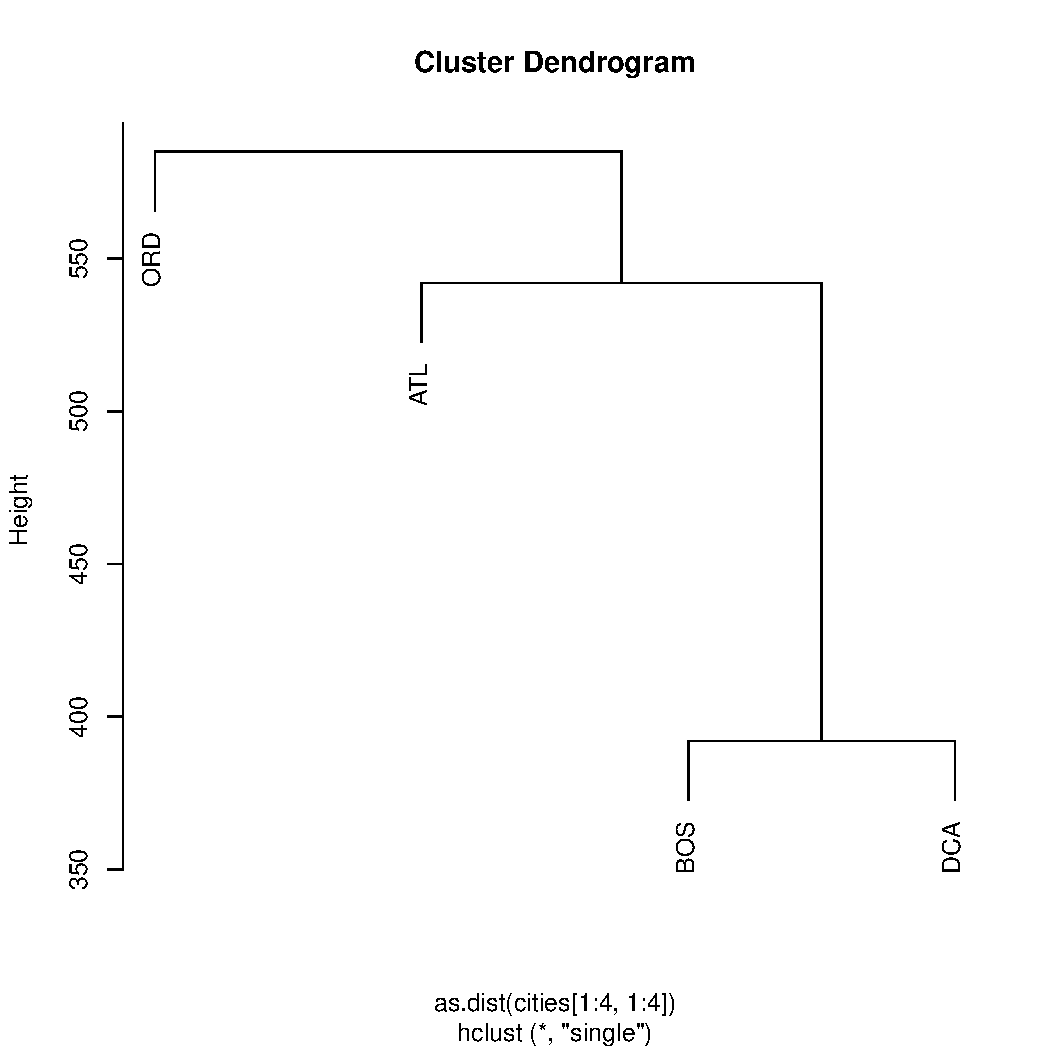
\includegraphics[width=.6\linewidth]{figure/beamer-apsing-1} 

}



\end{knitrout}
\end{frame}



%% \begin{frame}
%%  \begin{figure}
%%    \frametitle{City Example (Single Linkage)}
%%     \centering
%%     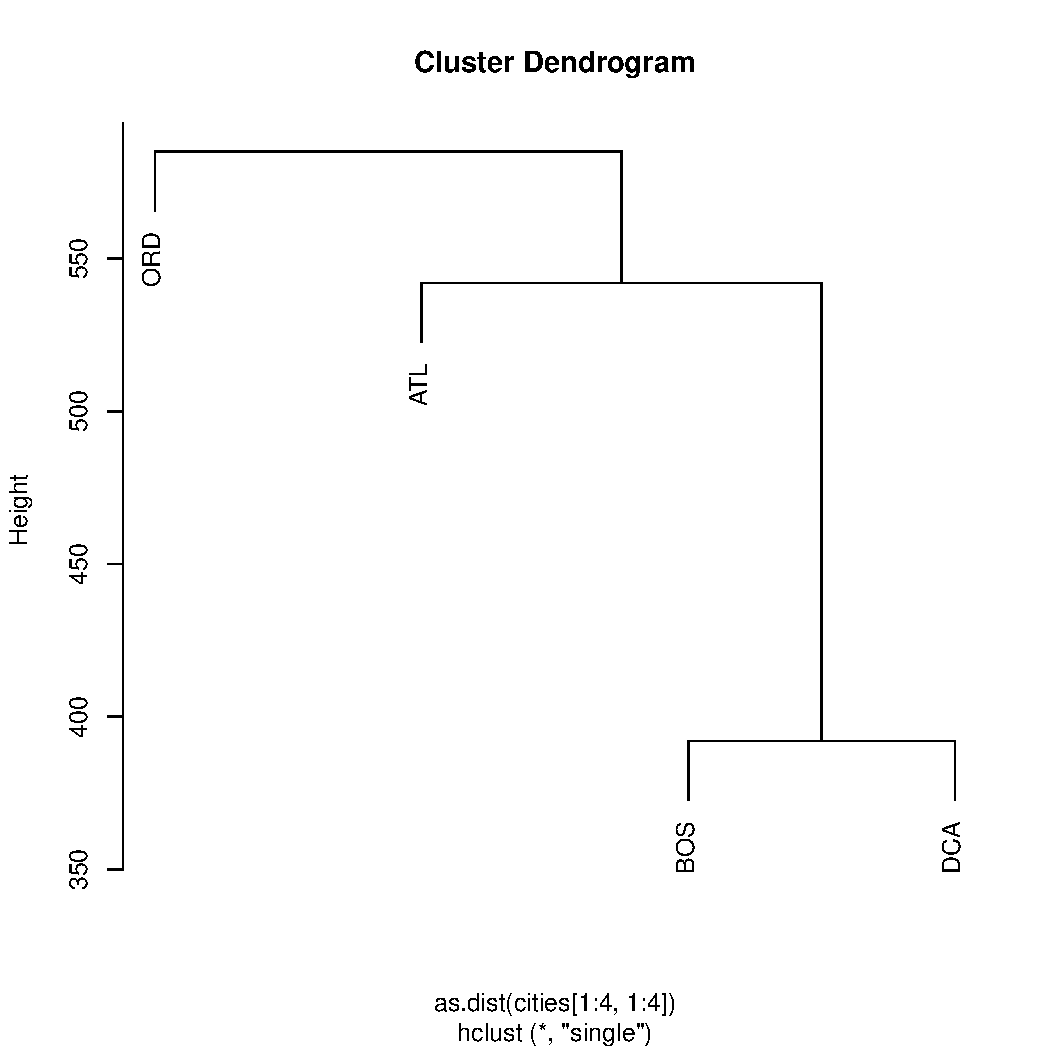
\includegraphics[scale=0.45]{Figures/dendcity.pdf}
%%   \end{figure}

%% \end{frame}




\begin{frame}
  \frametitle{Clustering Cities by Distances (complete linkage)}
  \begin{table}[!htbp]
    \centering
   \begin{tabular}{lllll}
   & ATL&BOS&ORD& DCA\\
ATL&  0 &934&585&542\\
BOS& 934&  0&853& 392\\
ORD& 585&853&  0& 598\\
DCA& 542&392& 598&   0
\\ \hline
       &DCA-BOS&ATL&ORD\\
DCA-BOS&0      &934&853   \\
ATL    &934    &0  &585\\
ORD    &853       &585&0
\\ \hline
          &DCA-BOS&ATL-ORD\\
DCA-BOS&0          &934   \\
ATL-ORD&934       &0
\end{tabular}
\end{table}
\end{frame}


\begin{frame}[fragile]{Four Airports (complete linkage)}
\begin{knitrout}\tiny
\definecolor{shadecolor}{rgb}{0.969, 0.969, 0.969}\color{fgcolor}

{\centering 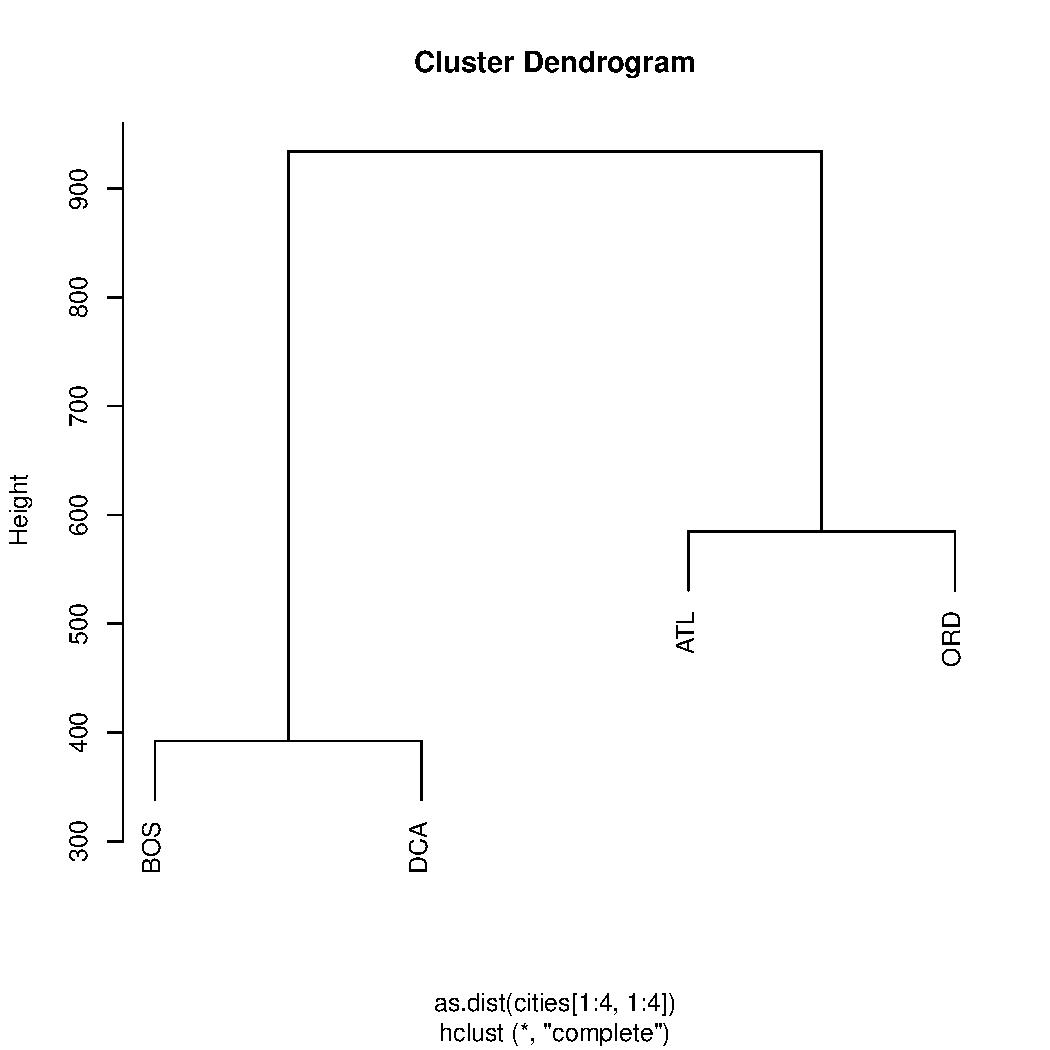
\includegraphics[width=.6\linewidth]{figure/beamer-apcomp-1} 

}



\end{knitrout}
\end{frame}

\begin{frame}{Four Airports (side by side)}
  \begin{table}[!htb]
    \tiny
      \centering
          \begin{tabular}{lllll}
   & ATL&BOS&ORD& DCA\\
ATL&  0 &934&585&542\\
BOS& 934&  0&853& 392\\
ORD& 585&853&  0& 598\\
DCA& 542&392& 598&   0
\\ \hline
       &DCA-BOS&ATL&ORD\\
DCA-BOS&0      &934&853   \\
ATL    &934    &0  &585\\
ORD    &853       &585&0
\\ \hline
          &DCA-BOS&ATL-ORD\\
DCA-BOS&0          &934   \\
ATL-ORD&934       &0
\end{tabular}
\caption{Complete Linkage}
\end{table}
\begin{table}[!htb]
    \tiny
      \centering
        \begin{tabular}{lllll}
   & ATL&BOS&ORD& DCA\\
ATL&  0 &934&585&542\\
BOS& 934&  0&853& 392\\
ORD& 585&853&  0& 598\\
DCA& 542&392& 598&   0
\\ \hline
       &DCA-BOS&ATL&ORD\\
DCA-BOS&0      &542&598   \\
ATL    &542    &0  &585\\
ORD    &598       &585&0
\\ \hline
           &DCA-BOS-ATL&ORD\\
DCA-BOS-ATL&0          &585   \\
ORD        &585        &0
\end{tabular}
\caption{Single Linkage}    
\end{table}
\end{frame}




\begin{frame}[fragile]{All Airports (comparison)}
\begin{knitrout}\tiny
\definecolor{shadecolor}{rgb}{0.969, 0.969, 0.969}\color{fgcolor}

{\centering 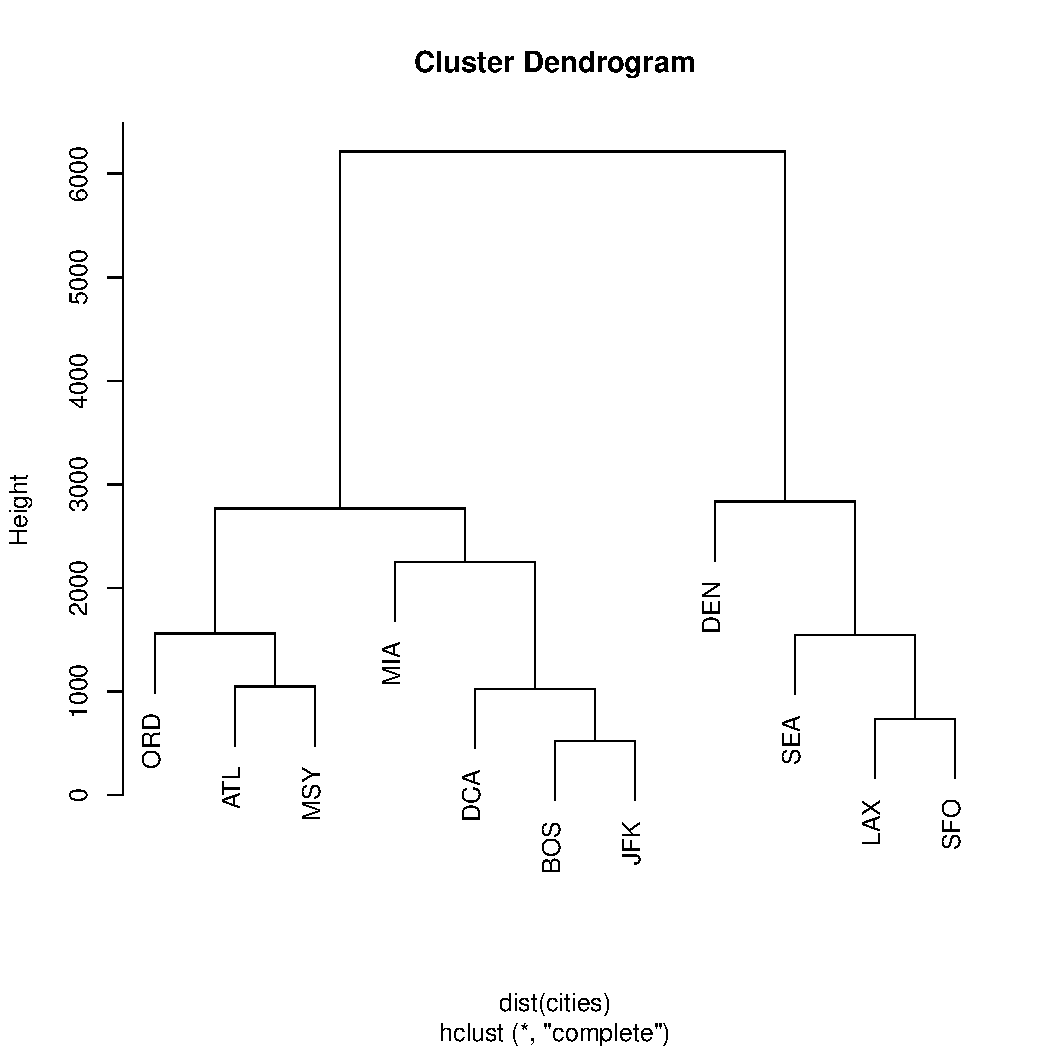
\includegraphics[width=.6\linewidth]{figure/beamer-airport3-1} 
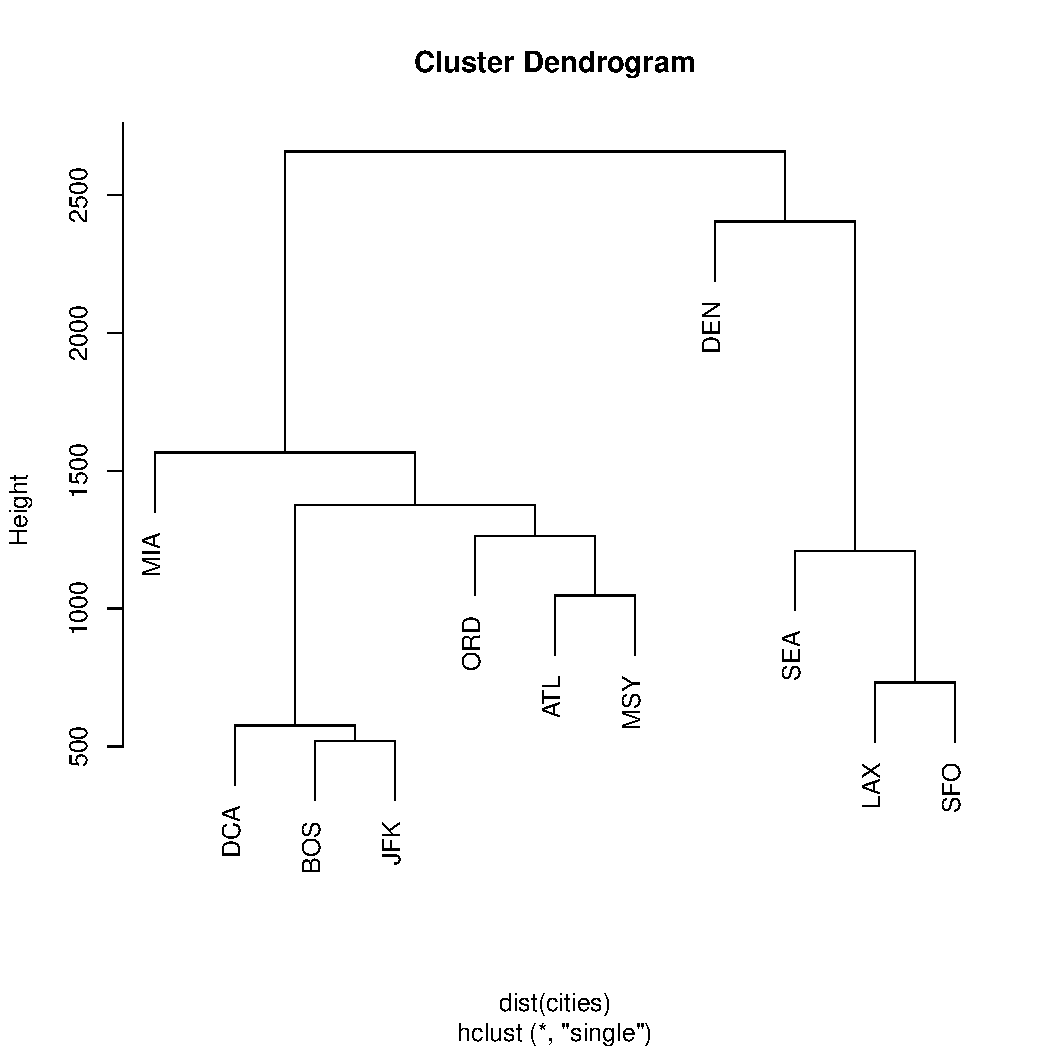
\includegraphics[width=.6\linewidth]{figure/beamer-airport3-2} 

}



\end{knitrout}
\end{frame}


\begin{frame}
  \frametitle{$k$-means Clustering}
  \begin{itemize}
\item Specify a number of potential clusters ($k$)
\item Split of the data (either randomly or based on some previous results) into $k$ partitions
\item Compute the mean (aka centroid) for each partition
\item For the first point (sample) determine the {\it nearest} centroid
\item The closeness is typically quantified using the Euclidean distance
\item Assign that point to that center
\item Repeat for points 2 through $n$
\item Assess the fit using the intra-cluster variance
\item Repeat as needed.
\end{itemize}
\end{frame}
\begin{frame}
  \frametitle{$k$-means Illustration}
\begin{figure}
   \centering
   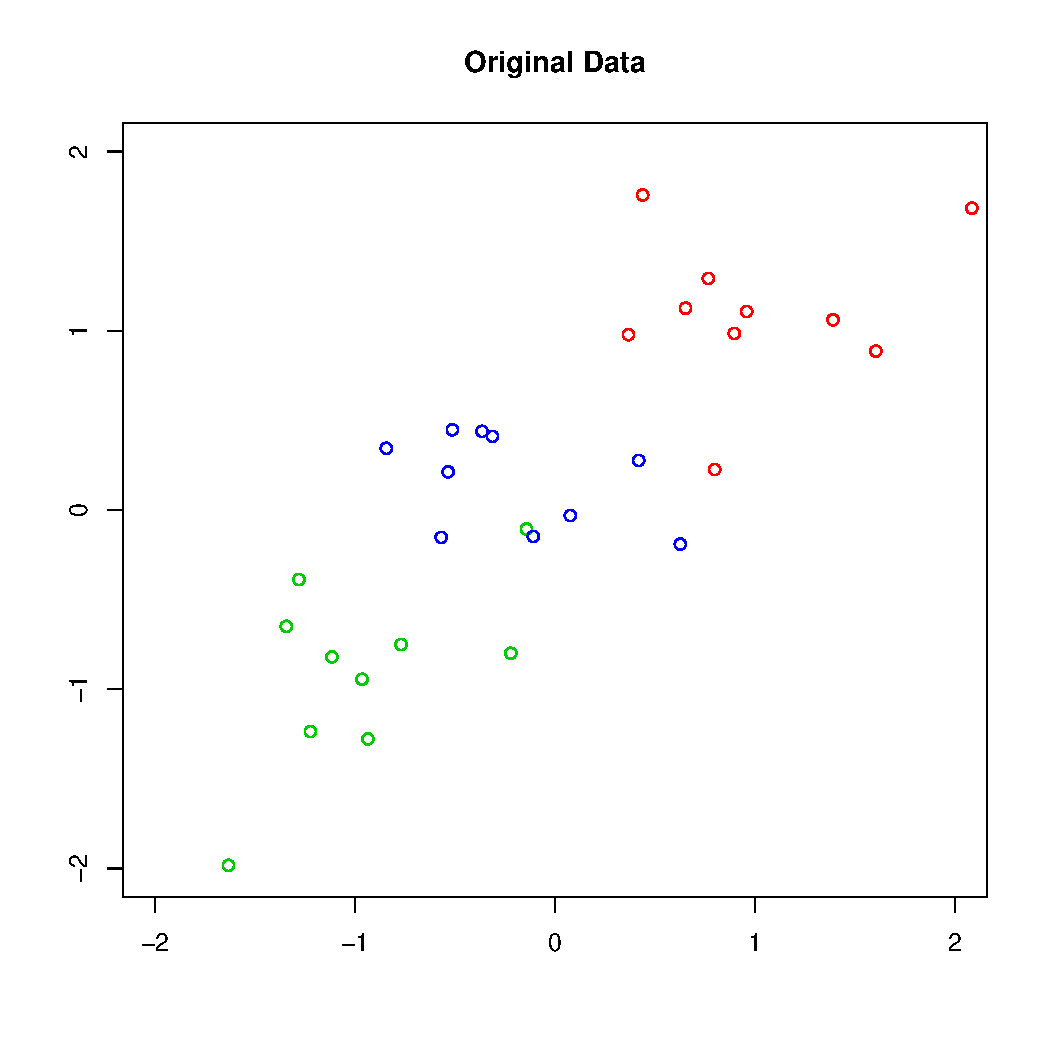
\includegraphics[scale=0.45]{Figures/kmean1.pdf}
 \end{figure}

\end{frame}

\begin{frame}
  \frametitle{$k$-means Illustration}
\begin{figure}
   \centering
   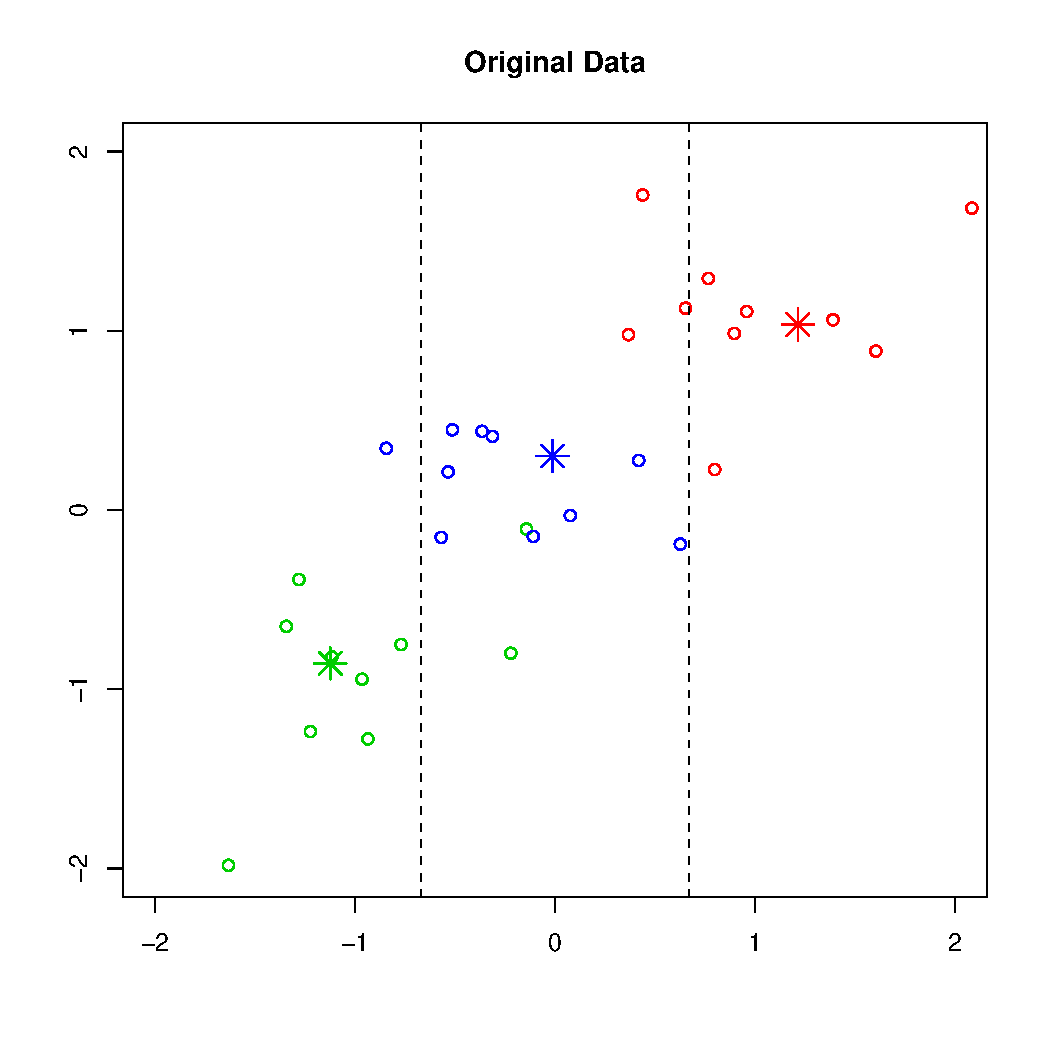
\includegraphics[scale=0.45]{Figures/kmean11.pdf}
 \end{figure}

\end{frame}


\begin{frame}
  \frametitle{$k$-means Illustration}
\begin{figure}
   \centering
   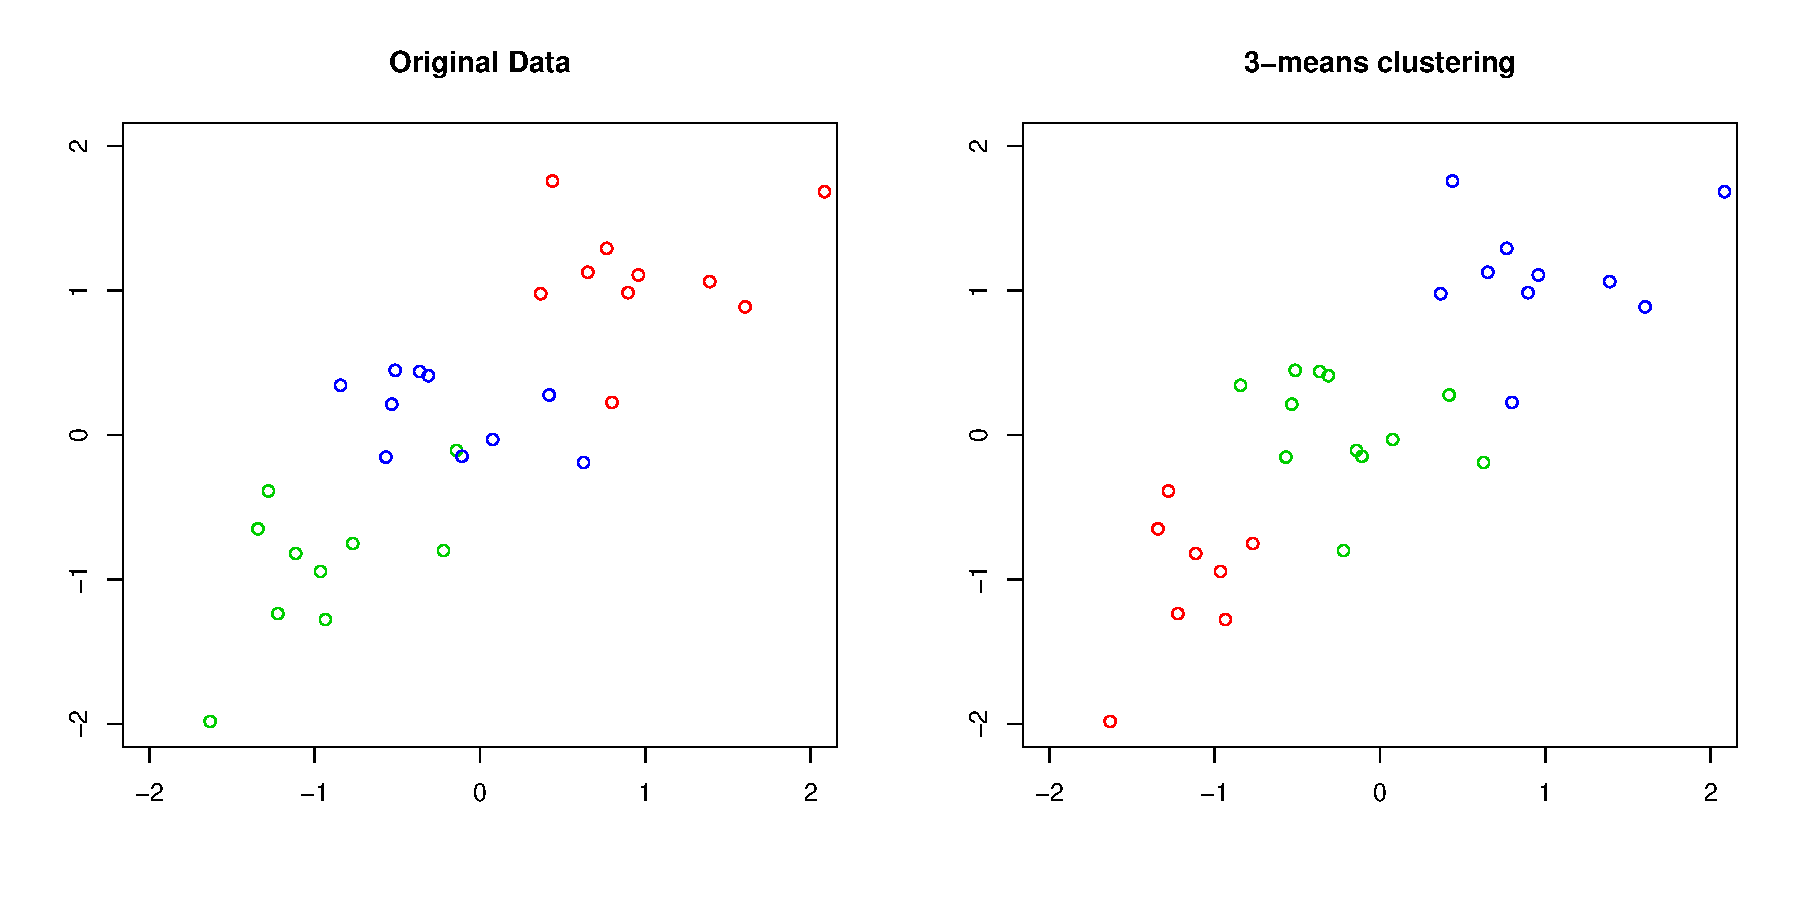
\includegraphics[scale=0.38]{Figures/kmean3.pdf}
 \end{figure}

\end{frame}

\begin{frame}
  \frametitle{$k$-means}
  \begin{itemize}
\item This is an example of {\it non-hierarchical} clustering
\item Need to specify the number of clusters up front
\item Need to specify (deterministically or randomly) the 
      centers of the clusters up front
\item Results are sensitive to the choice of $k$ and initial partitions
\item There is a relationship between $k$-means and PCA.
\end{itemize}
\end{frame}



\begin{frame}
  \frametitle{Batch Effect Discovery}
  \begin{itemize}
\item The MDS method is very useful for detecting batch effects
\item Batch effects tend to be stronger that biological effects
\item They also affect most probe sets (the biological effect may only be captured by a few)
\item This can be an effective weapon in your QC arsenal (this is how I start any new analysis)
\end{itemize}
\end{frame}

\begin{frame}{From CCR 2008 Paper}
   \begin{figure}
   \centering
   \includegraphics[scale=0.45]{Figures/CCR-FIG1.pdf}
 \end{figure}
  
\end{frame}
\begin{frame}
  \frametitle{ALL/AML Data}

  \begin{figure}
   \centering
   \includegraphics[scale=0.45]{Figures/CTS-ALLAML-MDS.pdf}
 \end{figure}

\end{frame}

\begin{frame}
  \frametitle{Semi-supervised Learning}
  \begin{itemize}
\item Heatmap illustration:
  \begin{itemize}
  \item Select a panel of probe-sets based on the two-sample $t$-test
  \item Carry out hierarchical clustering with respect to the patients (the columns)
  \item Carry out hierarchical clustering with respect to the probe sets in the panel (the rows)
  \item Present the results using a heatmap
  \end{itemize}
\item Some consider this an {\it unsupervised} analysis as the hierarchical clustering algorithm
      is unaware of the classes
\item This is not an accurate assessment: It is semi-supervised in the sense that we are picking
      genes based on the phenotype
\item A procedure is {\it unsupervised} if the class info is only used for annotation
\end{itemize}
\end{frame}



\begin{frame}[containsverbatim]
  \frametitle{{\tt R} Code to simulate Heatmap}
\footnotesize
\begin{knitrout}\tiny
\definecolor{shadecolor}{rgb}{0.969, 0.969, 0.969}\color{fgcolor}\begin{kframe}
\begin{alltt}
\hlstd{simulate.noise.heatmap}\hlkwb{=}\hlkwa{function}\hlstd{(}\hlkwc{n}\hlstd{,}\hlkwc{m}\hlstd{,}\hlkwc{alpha}\hlstd{)}
  \hlstd{\{}
    \hlcom{# Simulate Expression Matrix}
    \hlstd{EXPRS}\hlkwb{=}\hlkwd{matrix}\hlstd{(}\hlkwd{rnorm}\hlstd{(}\hlnum{2}\hlopt{*}\hlstd{n}\hlopt{*}\hlstd{m),m,}\hlnum{2}\hlopt{*}\hlstd{n)}
    \hlstd{grp}\hlkwb{=}\hlkwd{factor}\hlstd{(}\hlkwd{rep}\hlstd{(}\hlnum{0}\hlopt{:}\hlnum{1}\hlstd{,}\hlkwd{c}\hlstd{(n,n)))}
    \hlkwd{rownames}\hlstd{(EXPRS)}\hlkwb{=}\hlkwd{paste}\hlstd{(}\hlstr{"Gene"}\hlstd{,}\hlnum{1}\hlopt{:}\hlstd{m,}\hlkwc{sep}\hlstd{=}\hlstr{""}\hlstd{)}
    \hlkwd{colnames}\hlstd{(EXPRS)}\hlkwb{=}\hlkwd{paste}\hlstd{(}\hlstr{"patient id"}\hlstd{,}\hlnum{1}\hlopt{:}\hlstd{(}\hlnum{2}\hlopt{*}\hlstd{n),}\hlkwc{sep}\hlstd{=}\hlstr{""}\hlstd{)}

    \hlcom{# Get the two sample t-statistics}
    \hlstd{pvals}\hlkwb{=}\hlkwd{rowttests}\hlstd{(EXPRS, grp)}\hlopt{$}\hlstd{p.value}
    \hlstd{topgenes}\hlkwb{=}\hlkwd{which}\hlstd{(pvals}\hlopt{<}\hlstd{alpha)}
    \hlstd{EXPRS}\hlkwb{=}\hlstd{EXPRS[topgenes,]}
    \hlstd{annodat}\hlkwb{=}\hlkwd{data.frame}\hlstd{(}\hlkwc{Condition}\hlstd{=}\hlkwd{ifelse}\hlstd{(grp}\hlopt{==}\hlnum{0}\hlstd{,}\hlstr{"N"}\hlstd{,}\hlstr{"Y"}\hlstd{),}\hlkwc{row.names}\hlstd{=}\hlkwd{colnames}\hlstd{(EXPRS))}
    \hlkwd{pheatmap}\hlstd{(EXPRS,}
             \hlkwc{border_color} \hlstd{=}\hlnum{NA}\hlstd{,}
             \hlkwc{show_rownames} \hlstd{=} \hlnum{FALSE}\hlstd{,}
             \hlkwc{show_colnames}\hlstd{=}\hlnum{FALSE}\hlstd{,}
             \hlkwc{annotation_col}\hlstd{=annodat,}
             \hlkwc{color}\hlstd{=}\hlkwd{colorRampPalette}\hlstd{(}\hlkwd{c}\hlstd{(}\hlstr{"red3"}\hlstd{,} \hlstr{"black"}\hlstd{,} \hlstr{"green3"}\hlstd{))(}\hlnum{50}\hlstd{),}
             \hlkwc{annotation_colors}\hlstd{=}\hlkwd{list}\hlstd{(}\hlkwc{Condition}\hlstd{=}\hlkwd{c}\hlstd{(}\hlkwc{Y}\hlstd{=}\hlstr{"blue"}\hlstd{,}\hlkwc{N}\hlstd{=}\hlstr{"yellow"}\hlstd{)))}
    \hlkwd{return}\hlstd{(}\hlkwd{length}\hlstd{(topgenes))}
  \hlstd{\}}
\end{alltt}
\end{kframe}
\end{knitrout}
\end{frame}


\begin{frame}[containsverbatim]
  \frametitle{Heatmap Example: $m=20,000, n=20$, $\alpha=0.005$}
\begin{knitrout}\tiny
\definecolor{shadecolor}{rgb}{0.969, 0.969, 0.969}\color{fgcolor}

{\centering \includegraphics[width=.5\linewidth]{figure/beamer-hm1-1} 

}



\end{knitrout}

\end{frame}


\begin{frame}[containsverbatim]
  \frametitle{Heatmap Example: $m=40,000, n=20$, $\alpha=0.0025$}

\begin{knitrout}\tiny
\definecolor{shadecolor}{rgb}{0.969, 0.969, 0.969}\color{fgcolor}

{\centering \includegraphics[width=.5\linewidth]{figure/beamer-hm2-1} 

}



\end{knitrout}
\end{frame}


\begin{frame}[containsverbatim]
  \frametitle{Heatmap Example: $m=20,000, n=3$, $\alpha=0.005$}

\begin{knitrout}\tiny
\definecolor{shadecolor}{rgb}{0.969, 0.969, 0.969}\color{fgcolor}

{\centering \includegraphics[width=.5\linewidth]{figure/beamer-hm3-1} 

}



\end{knitrout}
\end{frame}



\begin{frame}[containsverbatim]
  \frametitle{{\tt R} Code to simulate PC}
\footnotesize
\begin{knitrout}\tiny
\definecolor{shadecolor}{rgb}{0.969, 0.969, 0.969}\color{fgcolor}\begin{kframe}
\begin{alltt}
\hlstd{simulate.noise.PC}\hlkwb{=}\hlkwa{function}\hlstd{(}\hlkwc{n}\hlstd{,}\hlkwc{m}\hlstd{,}\hlkwc{alpha}\hlstd{)}
  \hlstd{\{}
    \hlcom{# Simulate Expression Matrix}
    \hlstd{EXPRS}\hlkwb{=}\hlkwd{matrix}\hlstd{(}\hlkwd{rnorm}\hlstd{(}\hlnum{2}\hlopt{*}\hlstd{n}\hlopt{*}\hlstd{m),m,}\hlnum{2}\hlopt{*}\hlstd{n)}
    \hlstd{grp}\hlkwb{=}\hlkwd{factor}\hlstd{(}\hlkwd{rep}\hlstd{(}\hlnum{0}\hlopt{:}\hlnum{1}\hlstd{,}\hlkwd{c}\hlstd{(n,n)))}
    \hlcom{# Get the two sample t-statistics}
    \hlstd{pvals}\hlkwb{=}\hlkwd{rowttests}\hlstd{(EXPRS, grp)}\hlopt{$}\hlstd{p.value}
    \hlstd{topgenes}\hlkwb{=}\hlkwd{which}\hlstd{(pvals}\hlopt{<}\hlstd{alpha)}
    \hlstd{EXPRS}\hlkwb{=}\hlstd{EXPRS[topgenes,]}
    \hlstd{annodat}\hlkwb{=}\hlkwd{data.frame}\hlstd{(}\hlkwc{Condition}\hlstd{=}\hlkwd{ifelse}\hlstd{(grp}\hlopt{==}\hlnum{0}\hlstd{,}\hlstr{"N"}\hlstd{,}\hlstr{"Y"}\hlstd{),}\hlkwc{row.names}\hlstd{=}\hlkwd{colnames}\hlstd{(EXPRS))}
    \hlstd{PC}\hlkwb{=}\hlkwd{cmdscale}\hlstd{(}\hlkwd{dist}\hlstd{(}\hlkwd{t}\hlstd{(EXPRS)))}
    \hlkwd{plot}\hlstd{(PC,}\hlkwc{xlab}\hlstd{=}\hlstr{"PC1"}\hlstd{,}\hlkwc{ylab}\hlstd{=}\hlstr{"PC2"}\hlstd{,}\hlkwc{col}\hlstd{=}\hlkwd{ifelse}\hlstd{(grp}\hlopt{==}\hlnum{0}\hlstd{,}\hlstr{"yellow"}\hlstd{,}\hlstr{"blue"}\hlstd{),}\hlkwc{pch}\hlstd{=}\hlnum{19}\hlstd{)}
    \hlkwd{return}\hlstd{(}\hlkwd{length}\hlstd{(topgenes))}
\hlstd{\}}
\end{alltt}
\end{kframe}
\end{knitrout}
\end{frame}


\begin{frame}[containsverbatim]
  \frametitle{Heatmap Example: $K=20000, n=20$, $\alpha=0.005$}
\begin{knitrout}\tiny
\definecolor{shadecolor}{rgb}{0.969, 0.969, 0.969}\color{fgcolor}

{\centering \includegraphics[width=.5\linewidth]{figure/beamer-pc1-1} 

}



\end{knitrout}

\end{frame}


\begin{frame}[containsverbatim]
  \frametitle{Heatmap Example: $K=40000, n=20$, $\alpha=0.0025$}

\begin{knitrout}\tiny
\definecolor{shadecolor}{rgb}{0.969, 0.969, 0.969}\color{fgcolor}

{\centering \includegraphics[width=.5\linewidth]{figure/beamer-pc2-1} 

}



\end{knitrout}
\end{frame}


\begin{frame}[containsverbatim]
  \frametitle{Heatmap Example: $K=20000, n=3$, $\alpha=0.005$}

\begin{knitrout}\tiny
\definecolor{shadecolor}{rgb}{0.969, 0.969, 0.969}\color{fgcolor}

{\centering \includegraphics[width=.5\linewidth]{figure/beamer-pc3-1} 

}



\end{knitrout}








\end{frame}



\begin{frame}{Reminder: A Self-fulfilling Prophecy}
  \begin{itemize}
  \item Statistical method for unsupervised learning guarantee one thing
  \item They will return a clustering of your data
  \item What they do not guarantee and are invariably unable to 
        verify, is the biological relevance or reproducibility of the clustering
  \item In light of this Self-fulfilling Prophecy, these methods should be used
      with utmost care
  \end{itemize}
\end{frame}



\section[Multiple Testing]{Elements of Multiple Testing}

\begin{frame}[fragile]{Multiple Testing: Motivation}
  \begin{itemize}
  \item Flip a single coin from a large batch of newly minted coins 10 times
  \end{itemize}
\begin{knitrout}\tiny
\definecolor{shadecolor}{rgb}{0.969, 0.969, 0.969}\color{fgcolor}\begin{kframe}
\begin{verbatim}
##  [1] "T" "T" "T" "T" "T" "T" "T" "H" "T" "T"
\end{verbatim}
\end{kframe}
\end{knitrout}
\begin{itemize}
\item Is this a biased coin?
\end{itemize}
\begin{knitrout}\tiny
\definecolor{shadecolor}{rgb}{0.969, 0.969, 0.969}\color{fgcolor}\begin{kframe}
\begin{verbatim}
## 
## 	Exact binomial test
## 
## data:  sum(x == "T") and length(x)
## number of successes = 9, number of trials = 10, p-value = 0.02148
## alternative hypothesis: true probability of success is not equal to 0.5
## 95 percent confidence interval:
##  0.5549839 0.9974714
## sample estimates:
## probability of success 
##                    0.9
\end{verbatim}
\end{kframe}
\end{knitrout}
\end{frame}



\begin{frame}[fragile]{Multiple Testing: Motivation}
  \begin{itemize}
  \item Flip two coins each 10 times
  \end{itemize}
\begin{knitrout}\tiny
\definecolor{shadecolor}{rgb}{0.969, 0.969, 0.969}\color{fgcolor}\begin{kframe}
\begin{verbatim}
##  [1] "T" "T" "T" "T" "T" "T" "T" "H" "T" "T"
##  [1] "T" "H" "T" "H" "H" "H" "T" "T" "H" "H"
\end{verbatim}
\end{kframe}
\end{knitrout}
\begin{itemize}
\item Are any of the two coins biased?
\end{itemize}
\begin{knitrout}\tiny
\definecolor{shadecolor}{rgb}{0.969, 0.969, 0.969}\color{fgcolor}\begin{kframe}
\begin{alltt}
\hlkwd{binom.test}\hlstd{(}\hlkwd{sum}\hlstd{(x1}\hlopt{==}\hlstr{'T'}\hlstd{),} \hlkwc{n}\hlstd{=}\hlkwd{length}\hlstd{(x),} \hlkwc{p} \hlstd{=} \hlnum{0.5}\hlstd{)}
\end{alltt}
\begin{verbatim}
## 
## 	Exact binomial test
## 
## data:  sum(x1 == "T") and length(x)
## number of successes = 9, number of trials = 10, p-value = 0.02148
## alternative hypothesis: true probability of success is not equal to 0.5
## 95 percent confidence interval:
##  0.5549839 0.9974714
## sample estimates:
## probability of success 
##                    0.9
\end{verbatim}
\begin{alltt}
\hlkwd{binom.test}\hlstd{(}\hlkwd{sum}\hlstd{(x2}\hlopt{==}\hlstr{'T'}\hlstd{),} \hlkwc{n}\hlstd{=}\hlkwd{length}\hlstd{(x),} \hlkwc{p} \hlstd{=} \hlnum{0.5}\hlstd{)}
\end{alltt}
\begin{verbatim}
## 
## 	Exact binomial test
## 
## data:  sum(x2 == "T") and length(x)
## number of successes = 4, number of trials = 10, p-value = 0.7539
## alternative hypothesis: true probability of success is not equal to 0.5
## 95 percent confidence interval:
##  0.1215523 0.7376219
## sample estimates:
## probability of success 
##                    0.4
\end{verbatim}
\end{kframe}
\end{knitrout}

\end{frame}




\begin{frame}
  \frametitle{Multiple Testing}
  \begin{itemize}
      \item We have previously considered testing for significance of a single gene
      \item The analysis of high-dimensional data, including array and sequencing data,
            is concerned with testing the significance of multiple loci/genes
            \begin{itemize}
            \item Microarray : 20,000-50,000 probe sets
            \item GWAS:        500,000-5,000,000 typed SNPs
            \item RNA-Seq:     22,000 genes (humans), ? genes (ecoli)
            \end{itemize}
      \item Let $m$ denote the number of genes (or SNPs) to be tested
      \item Rather than testing a single hypothesis, we are concerned with testing multiple hypotheses
      \item The decision rule must now account for testing $m$ hypotheses  simultaneously (multiple testing)
  \end{itemize}
\end{frame}


\begin{frame}{Hypothesis Notation}
  \begin{itemize}
  \item Gene $j$ (among the $m$ genes) is either associated with the outcome or not
  \item The truth is unknown to us                                     
  \item The null hypothesis for gene $j$ is denoted by $H_j$ (gene $j$ is 
  \item $H_j$: gene $j$ is not associated with the outcome of interest
  \item The alternative hypothesis is denoted by $\bar{H}_j$
  \item $\bar{H}_j$: gene $j$ is associated with the outcome of interest
  \item Suppose that we only test a single gene, say gene $j$, among the $m$
        genes
  \item Let $p_j$ (lower case p) denote the corresponding {\it P}-value
  \item $p_j$ is called the {\it marginal}
        or {\it unadjusted} {\it P}-value
  \item 
  \end{itemize}
\end{frame}

\begin{frame}{Unadjusted vs Adjusted {\it P}-values}
  \begin{itemize}
  \item Suppose that we only test a single gene, say gene $j$, among the $m$
        genes
  \item Let $p_j$ (lower case p) denote {\it P}-value corresponding to $H_j$
  \item $p_j$ is called the {\it marginal} or {\it unadjusted} {\it P}-value
  \item If $m$ hypotheses are tested, inference on $H_j$ on the basis of
        $p_j$ is inappropriate
  \item The {\it P}-value for $H_j$ has to account for testing the other $m-1$ hypotheses
  \item We will denote the {\it adjusted} {\it P}-value by  $P_j$ (upper case P)
  \end{itemize}
\end{frame}


\begin{frame}{Additional Notation}
  \begin{itemize}
  \item Suppose that gene $j$ is not associated with the outcome of interest ($H_j$ is true)
  \item Then
    \begin{itemize}
    \item Decision rule rejects $\to$ False-Positive (FP) 
    \item Decision rule fails to reject $\to$ True-Negative (TN) 
    \end{itemize}
  \item Suppose that gene $j$ is associated with the outcome of interest ($H_j$ is false)
  \begin{itemize}
    \item Decision rule rejects $\to$ True-Positive (TP) 
    \item Decision rule fails to reject $\to$  False-Negative (FN) 
    \end{itemize}
  \end{itemize}
\end{frame}




\begin{frame}
  \frametitle{Summarizing a Multiple Testing Procedure}
  \begin{itemize}
\item The results from any multiple testing procedure can be summarized
      as the following table
  \begin{center}
  \begin{tabular}{r|c|c|c}
    & Accept & Reject & Total \\
   \cline{1-4}
  Truth Null & $A_0$ & $R_0$ & $m_0$ \\
  \cline{1-4}
  Alt. & $A_1$ & $R_1$ & $m_1$ \\
  \cline{1-4} 
    & $A$ & $R$ & $m$
  \end{tabular}
  \end{center}
  \item Notation:
    \begin{itemize}
    \item $m$: Number of tests, $m_0,m_1$ number of null/true genes
    \item $R$: Number of genes rejected according to the decision rule
    \item $A$: Number of genes accepted according to the decision rule
    \item $R_0/R_1$ number of TN/FP
    \item $A_0/A_1$ number of FN/TP
    \end{itemize}
    
    \end{itemize}

\end{frame}


\begin{frame}[fragile]{Example}
  \begin{itemize}
  \item Results from an analysis based on $m=10$ genes:  
\begin{knitrout}\tiny
\definecolor{shadecolor}{rgb}{0.969, 0.969, 0.969}\color{fgcolor}\begin{kframe}
\begin{verbatim}
##      gene truth  pvalue
## 1   gene1     0 0.29070
## 2   gene2     1 0.61630
## 3   gene3     1 0.00320
## 4   gene4     0 0.01641
## 5   gene5     0 0.25150
## 6   gene6     0 0.58450
## 7   gene7     0 0.22890
## 8   gene8     1 0.12630
## 9   gene9     0 0.26080
## 10 gene10     0 0.04980
\end{verbatim}
\end{kframe}
\end{knitrout}
\item Investigator decides to use following decision rule:
  Any gene with a corresponding unadjusted {\it P}-value of less than 0.05 will
  be rejected.
  \item Note:
    \begin{itemize}
 \item $m_0=7$ and $m_1=3$ 
  
  \item $R=3$ will be rejected based on the decision rule
  \item Consequently $A=m-R=7$ will be accepted
  \item $R_0=2,R_1=1, A_0=5$ and $A_1=2$
\end{itemize}
\end{itemize}

\end{frame}


\begin{frame}{Example: Fill in the 2x2 table}
 \begin{center}
  \begin{tabular}{r|c|c|c}
    & Accept & Reject & Total \\
   \cline{1-4}
  Truth Null  & $A_0=5$ & $R_0=2$ & $m_0=7$ \\
  \cline{1-4}
    Alt. & $A_1=2$ & $R_1=1$ & $m_1=3$ \\
  \cline{1-4} 
    & $A=7$ & $R=3$ & $m=10$
  \end{tabular}
  \end{center}
 
\end{frame}

\begin{frame}[fragile]{The Truth}
  \begin{itemize}
  \item What know or observe is this
\begin{knitrout}\tiny
\definecolor{shadecolor}{rgb}{0.969, 0.969, 0.969}\color{fgcolor}\begin{kframe}
\begin{verbatim}
##      gene  pvalue
## 1   gene1 0.29070
## 2   gene2 0.61630
## 3   gene3 0.00320
## 4   gene4 0.01641
## 5   gene5 0.25150
## 6   gene6 0.58450
## 7   gene7 0.22890
## 8   gene8 0.12630
## 9   gene9 0.26080
## 10 gene10 0.04980
\end{verbatim}
\end{kframe}
\end{knitrout}
\item and not (truth colum is not known to us):
\begin{knitrout}\tiny
\definecolor{shadecolor}{rgb}{0.969, 0.969, 0.969}\color{fgcolor}\begin{kframe}
\begin{alltt}
\hlstd{dat}
\end{alltt}
\begin{verbatim}
##      gene truth  pvalue
## 1   gene1     0 0.29070
## 2   gene2     1 0.61630
## 3   gene3     1 0.00320
## 4   gene4     0 0.01641
## 5   gene5     0 0.25150
## 6   gene6     0 0.58450
## 7   gene7     0 0.22890
## 8   gene8     1 0.12630
## 9   gene9     0 0.26080
## 10 gene10     0 0.04980
\end{verbatim}
\end{kframe}
\end{knitrout}
  \end{itemize}
\end{frame}



\begin{frame}{Example: Fill in the 2x2 table (based on what we observe)}
   \begin{itemize}
     \item We can only fill in the bottom row of the table
        \begin{center}
          \begin{tabular}{r|c|c|c}
            & Accept & Reject & Total \\
            \cline{1-4}
            Truth Null  & $A_0$ & $R_0$ & $m_0$ \\
            \cline{1-4}
            Alt. & $A_1$ & $R_1$ & $m_1$ \\
            \cline{1-4} 
            & $A=7$ & $R=3$ & $m=10$
     \end{tabular}
   \end{center}
 \item The remaining quantities are fixed unknown quantities or unobservable random variables.
   \end{itemize}
\end{frame}


\begin{frame}
   \frametitle{Framework of multiple testing}
  \begin{center}
  \begin{tabular}{r|c|c|c}
    & Accept & Reject & Total \\
   \cline{1-4}
  Truth Null  & $A_0$ & $R_0$ & $m_0$ \\
  \cline{1-4}
    Alt. & $A_1$ & $R_1$ & $m_1$ \\
  \cline{1-4} 
    & $A$ & $R$ & $m$
  \end{tabular}
  \end{center}
 
  \begin{itemize}
    \item $m$ is a known constant 
    \item $m_0$ and $m_1$ are unknown constants
    \item $R$ and $A$ are determined on the basis of applying the decision rule to the data
    \item They are {\it observable} random quantities
    \item The true states of the genes of the genes are unknown
    \item $A_0,A_1,R_0$ and $R_1$ are  {\it unobservable} random quantities
    \end{itemize}
\end{frame}

\begin{frame}
  \frametitle{Framework versus Method}
  \begin{itemize}
    \item To account for multiple testing one has to first decide on a framework and then
          on a method
    \item {\Large Framework:} The quantity that we aim to control
    \item {\Large Method:} statistical procedure used to for estimating or controlling the error 
      rate for a set of hypothesis tests.
    \item Example: Investment 
      \begin{itemize}
      \item What is the objective: capital preservation or growth
      \item Approach: Index funds, individual stocks, CDs, money under mattress
      \end{itemize}
   \item: When thinking of multiple testing, first decide what the framework is and then
          decide on an appropriate strategy
  \end{itemize}
\end{frame}


\begin{frame}{Family-wise Error Rate (FWER)}
  \begin{itemize}
  \item What is the probability to commit at least one false-rejection (among m) given that 
        {\it all} genes are null
  \item What is the the probability of the event $R\ge 1$ if $m=m_0$
  \item $\mathrm{FWER}=P(R\ge 1|m=m0)$
  \item Note that when $m=1$ (single gene), this definition is identical to the tyep I error
        we have previously considered
  \end{itemize}
\end{frame}

\begin{frame}{Bonferroni}
  \begin{itemize}
  \item A simple method for controlling FWER is called the Bonferroni method
  \item To control the type I error of the experiement at the 
        $\alpha$ level, test each gene at the $\frac{\alpha}{m}$ level
  \item The Bonferroni adjusted {\it P-value} is defined as
    \begin{equation*}
      P_j=m \times p_j
    \end{equation*}
  \item Technical note: $P_j$ is defined above could be larger than 1 so a more technically rigorous definition is
    \begin{equation*}
      P_j=\min\{m \times p_j,1\}
    \end{equation*}
  \item In other words, if $m \times p_j$ is larger than 1, then truncate $P_j$ at 1.
  \end{itemize}
\end{frame}


\begin{frame}{False Discovery Rate (FDR)}
  \begin{itemize}
  \item In the FWER framwork, the objective is to control $\mathrm{FWER}=P(R\ge 1|m=m0)$
  \item This is the probability of at least one false-discovery when none of the genes are true.
  \item Consider the quantity $\frac{R_0}{R}$
  \item This is the proportion of of false discoveries among the genes rejected
  \item This is an {\it unobservable} random quantity (As $R_0$ is not observable)
   \item In the FDR framework is based on controlling the {\it expected} value of this ratio
    \item The FDR is defined as $E[\frac{R_0}{R}]$
    \item Note that when $m_0=m$ (none of the genes are true), FWER=FDR
  \end{itemize}
\end{frame}


\begin{frame}{Methods for the FDR Framework}
  \begin{itemize}
  \item An early method proposed to control FDR, is a method due to
        Benjamini and Hochberg (BH; JRSBB 1985)
  \item One of the assumptions for the BH method is that of independence
        among the genes
  \item That assumption may be questionable (due to co-regulation among genes)
  \item A more recent approach is due to Storey
  \item The adjusted {\it P}-values calculated based on Storey's method
        are called {\it Q}-values
  \end{itemize}
\end{frame}


\begin{frame}{Genome-wide Significance}
  \begin{itemize}
  \item In GWAS papers, $\alpha=5\times 10^{-8}$ is typically considered
        the threshold for genome-wide significance
  \item It is based on a Bonferroni correction: If you consider testing $m=1,000,000$
        SNPs at the FWER level of 0.05, then each SNP should be tested at the
        \begin{equation*}
          \alpha=\frac{0.05}{1,000,000} = 5\times 10^{-8},
        \end{equation*}
        level
  \item Suppose that the unadjusted {\it P}=value for a SNP is $5\times 10^{-7}$
  \item Is this "reaching" genome-wide significance?
  \item The term "suggestive" is also used
  \end{itemize}
\end{frame}

\begin{frame}{"Reaching" Genome-wide Significance}
  \begin{itemize}
  \item Suppose that the $m=1,000,000$ SNPs are independent
  \item The adjusted {\it P}-value is
     \begin{equation*}
          P=5\times 10^{-7} \times m = 5\times 10^{-7} \times 10^6 = 0.5,
        \end{equation*}
  \item This is off by an order of magnitude ($0.5=0.05 \times 10$)
  \item It is not "reaching"
  \end{itemize}
\end{frame}


\begin{frame}
\frametitle{Summary of Multiple Testing}
\begin{itemize}
  \item Multiple testing {\em must} be accounted for when testing for associations in the context of high-dimensional data
  \item FWER and FDR are the two common frameworks for quantifying error
   
  \item Error rate estimates can be used to compute 'adjusted' p-values
   
  \item Resampling-based methods can increase power in controlling error when sample sizes are sufficient
    for their use.
  \item When large-scale patterns of differential expression are observed, it is important to consider if 
    such effects are biologically reasonable, and if technical factors can be attributed to the variation.
      \end{itemize}

\end{frame}



%% \begin{frame}
%%   \frametitle{Family-wise Error Rate (FWER)}
  
%%   \begin{center}
%%   \begin{tabular}{r|c|c|c}
%%     & Accept & Reject & Total \\
%%    \cline{1-4}
%%   Truth Null & $A_0$ & $R_0$ & $m_0$ \\
%%   \cline{1-4}
%%         Alt. & $A_1$ & $R_1$ & $m_1$ \\
%%   \cline{1-4} 
%%     & $A$ & $R$ & $m$
%%   \end{tabular}
%%   \end{center}
%%   \vskip5mm
%%   \begin{itemize}
%%     \item Defined as the probability of at least one false positive test result
%%       \begin{equation*}
%%     \mbox{FWER} = \mbox{Pr}(R_0 > 0)
%%       \end{equation*}
%%       \vskip2mm
%%     \item Because $R_0$, is unobservable, $FWER$ is unknown and therefore {\em estimated} or
%%       {\em controlled} in a given experiment.
%%       \vskip4mm
%%     \item Becomes a more stringent criterion as $m$ increases 
%%   \end{itemize}
%% \end{frame}
  


%% \begin{frame}
%%   \frametitle{Methods for controlling the FWER}
%%   \begin{itemize}
%%     \item Bonferroni correction \\
%%   \begin{equation*}
%%     \mbox{adjusted p:     } \tilde{p}_j = \min(m \cdot p_j, 1)  
%%   \end{equation*}      \vskip2mm
%%     \item Holm's step-down method\\
%%   \begin{equation*}      
%%     \mbox{adjusted p:     } \tilde{p}_{r_j} = \max_{k : 1, \ldots , j} \biggl[ 
%%      \min((m - k + 1) \cdot p_{r_k}, 1) \biggr]        
%%    \end{equation*}
%%   \vskip2mm
%%     \item Westfall-Young maxT method 
%%       \vskip2mm
%%       Resampling-based procedure that requires ${\bf X}$ and $Y$
%%   \end{itemize}
%% \end{frame}

%% \begin{frame}
%%   \frametitle{Aside: Correlation among genes}
%%   \begin{itemize} 
%%     \item {\em Many} of the traditional statistical approaches that are taken
%%       in the analysis of microarrays (and other 'omics data) make an
%%       implicit assumption of independence among genes under the global null.
%%            \vskip5mm     
%%     \item In differential expression, it can be stated as an assumption all
%%           test statistics are independent and identically distributed under the null.
%%           \begin{eqnarray}
%%              H_0: \; \; T_1, \; T_2, \; \ldots \; , \; T_m \; \; 
%%              \mbox{are {\em i.i.d.}  with} \; \; T_i \sim  F_0(t)  \nonumber
%%           \end{eqnarray}
%%            \vskip2mm     
%%     \item However, the scientific basis of microarrays is that genes are
%%       \alert{co-regulated} by biological processes - {\em even when these processes
%%       are independent of the association of interest}.
%%     \vskip5mm
%%     \item These data serve as the basis for identifying gene clusters, pathways and 
%%       ontologies (all to come).
%%       \end{itemize}
%%   \end{frame}
      
%% \begin{frame}
%%   \frametitle{Methods for controlling the FDR}
%%   \begin{itemize}
%%     \item Benjamini-Hochberg step-up \\
%%   \begin{equation*}
%%     \mbox{adjusted p:     } \tilde{p}_{r_j} = \min_{k : j, \ldots , m} \biggl[ 
%%      \min((m - k + 1) \cdot p_{r_k}, 1) \biggr]  
%%   \end{equation*}
%%       \vskip2mm
%%     \item Storey q-value (SAM)
%%      \begin{equation*}
%%     \widehat{FDR}(\alpha) = \frac{\hat{m}_0 \cdot \alpha}{R(\alpha)} 
%%   \end{equation*}   
%%       \vskip2mm
%%     \item Benjamini-Yekutieli 
%%       \vskip2mm
%%       Resampling-based procedure that requires ${\bf X}$ and $Y$
%%   \end{itemize}
%% \end{frame}

%% \begin{frame}
%%   \frametitle{Example: Beer data set}
%% In the earlier example of lung adenocarcinoma (Beer {\em et al.}), survival analysis was used to 
%% identify differentially expressed genes associated with clinical outcome.
%% \vskip5mm 
%% Tests for all $m = 7129$ probe sets can be summarized by tabulating genes ordered by the
%% degree of association. {\em I.e. genelist}
%% \vskip 5mm
%%     \begin{center}    {\scriptsize
%%     \begin{tabular}{|l|r|r|r|r|} \hline
%%      & {\bf  PROBESET}  & {\bf  GENE } & {\bf X.STAT  }  & {\bf PVAL} \\ \hline
%% 1 &    L34838\_at &   INSL4 &  38.28  &  6e-10\\
%% 2 &    U33147\_at & SCGB2A2 &  24.80 &   6e-07\\
%% 3 &  X03363\_s\_at &   ERBB2 &  20.46  &  6e-06\\
%% 4 &    K03195\_at &  SLC2A1 &  20.44  &  6e-06\\
%% 5 &    U33017\_at &  SLAMF1 &  18.38  &  2e-05\\
%% 6 &    D14874\_at &     ADM &  18.12  &  2e-05\\
%% 7  &   X16901\_at &  GTF2F2 &  17.35  &  3e-05\\
%% 8 &    U81607\_at &  AKAP12 &  16.73 &   4e-05\\
%% 9 &    Y08564\_at &    <NA> &  16.13 &   6e-05\\
%% 10 & U49957\_s\_at &     LPP &  14.92 & 0.00011\\\hline
%%     \end{tabular} 
%%     }
%%     \end{center}
%% \end{frame}

%% \begin{frame}
%%   \frametitle{Example: Beer data set}
%%   A histogram of the 7129 p-values is indicative of the extent of differential expression. 
%%   \begin{center}
%%   \vspace{-5mm}
%%   \includegraphics[width=60mm,height=50mm,trim=0in 0in 0in 0.5in,clip]{Figures/HistBeer.pdf}
%%   \end{center}
%% 686 genes are observed to have {\em nominal} $p < 0.05$ 
%% \end{frame}


%% \begin{frame}
%%   \frametitle{Example: Beer data set  }
%% Using the {\em multtest} package in Bioconductor, adjusted p-values are computed to control 
%% \begin{itemize}
%%   \item FWER - Holm's step-down 
%%   \item FDR - Benjamini-Hochberg step-up
%%     \end{itemize}
%% \vskip2mm
%%     \begin{center}    {\scriptsize
%%     \begin{tabular}{|l|r|r|r|r|r|r|} \hline
%%      & {\bf  PROBESET}  & {\bf  GENE } & {\bf X.STAT  }  & {\bf PVAL}& {\bf ADJP.FDR}& {\bf ADJP.FWER} \\ \hline
%% 1 &  L34838\_at  & INSL4 &38.28 & 6e-10  &  4e-06 &   4e-06\\
%% 2 &  U33147\_at  &SCGB2A2&24.80 & 6e-07  & 0.0023 &  0.0045\\
%% 3 &X03363\_s\_at & ERBB2 &20.46 & 6e-06  &  0.011 &  0.0434\\
%% 4 &  K03195\_at  &SLC2A1 &20.44 & 6e-06  &  0.011 &  0.0438\\
%% 5 &  U33017\_at  &SLAMF1 &18.38 & 2e-05  & 0.0246 &  0.1289\\
%% 6 &  D14874\_at  &   ADM &18.12 & 2e-05  & 0.0246 &  0.1478\\
%% 7 &  X16901\_at  &GTF2F2 &17.35 & 3e-05  & 0.0317 &  0.2215\\
%% 8 &  U81607\_at  &AKAP12 &16.73 & 4e-05  & 0.0384 &  0.3069\\
%% 9 &  Y08564\_at  &  <NA> &16.13 & 6e-05  & 0.0468 &  0.4211\\
%% 10& U49957\_s\_at&   LPP &14.92 & 0.00011& 0.0773 &  0.7986\\\hline
%%     \end{tabular} 
%%     }
%%     \end{center}
%% \end{frame}



%% \begin{frame}[containsverbatim]
%%   \frametitle{Example: AML versus ALL }
%% For the Golub dataset, Welch t-tests were used to 
%% identify differentially expressed genes between leukemia subtypes.

%% {\scriptsize 
%% \begin{verbatim}
%%      > library(golubEsets); library(affy)
%%      > data(Golub_Merge)
%%      > 
%%      > data <- exprs(Golub_Merge)
%%      > pheno <- pData(Golub_Merge)$ALL.AML
%%      > table(pheno)
%%      pheno
%%      ALL AML 
%%       47  25 
%%      > 
%%      > get.t <- function(x,y) t.test(x[y],x[!y])$statistic
%%      > get.p <- function(x,y) t.test(x[y],x[!y])$p.value
%%      > 
%%      > t.vec <- apply(data,1,get.t,pheno=="ALL")
%%      > p.vec <- apply(data,1,get.p,pheno=="ALL")
%%      > 
%%      > results <- data.frame(STAT     = t.vec,
%%      +                       PVAL     = p.vec)
%%      > 
%%      > results <- results[order(results$PVAL),]
%% \end{verbatim}
%% }
%% \end{frame}

%% \begin{frame}[containsverbatim]
%%   \frametitle{Example: AML versus ALL}
%% {\scriptsize 
%% \begin{verbatim}
%%      > library(multtest)
%%      > adj.p.FDR <- mt.rawp2adjp(results$PVAL, "BH")$adjp[,2]
%%      > adj.p.FWER <- mt.rawp2adjp(results$PVAL, "Holm")$adjp[,2]
%%      >
%%      > res.p.FWER <- mt.maxT(data, pheno=="ALL", B = 1000)$adjp
%% \end{verbatim}
%% \vskip2mm
%%     \begin{center}   
%%     \begin{tabular}{|l|r|r|r|r|r|} \hline
%%  {\bf  PROBESET}  & {\bf T.STAT  }  & {\bf PVAL} & {\bf ADJ.P.FDR} & {\bf ADJ.P.FWER} & {\bf RES.P.FWER} \\ \hline
%%          X59417\_at & 8.89 & 3e-12 & 2e-08 & 2e-08 & 0.001\\
%%          M92287\_at & 8.83 & 6e-12 & 2e-08 & 5e-08 & 0.001\\
%%          M31523\_at & 8.73 & 1e-11 & 3e-08 & 8e-08 & 0.001\\
%%       M31211\_s\_at & 7.99 & 2e-11 & 4e-08 & 1e-07 & 0.001\\
%%    U05259\_rna1\_at & 8.44 & 4e-11 & 6e-08 & 3e-07 & 0.001\\
%% M84371\_rna1\_s\_at & 8.12 & 5e-11 & 6e-08 & 3e-07 & 0.001\\
%%          J05243\_at & 7.87 & 8e-11 & 9e-08 & 6e-07 & 0.001\\
%%          M11722\_at & 7.99 & 2e-10 & 2e-07 & 2e-06 & 0.001\\
%%          M89957\_at & 7.73 & 3e-10 & 2e-07 & 2e-06 & 0.001\\
%%          S50223\_at & 7.43 & 3e-10 & 2e-07 & 2e-06 & 0.001\\\hline
%%     \end{tabular} 
%%     \end{center}
%%     }
%% \end{frame}



%% \begin{frame}[containsverbatim]
%%   \frametitle{Example: AML versus ALL}
%%   \begin{center}
%%   \includegraphics[width=60mm,height=50mm,trim=0in 0in 0in 0.75in,clip]{Figures/AdjpFWER.pdf}
%%   \end{center}
%%   Even though the resampling based adjustments to FWER are bounded by the number of permutations
%%   ($B = 1000$), the Westfall-Young method is more powerful than those that ignore correlation. 
%% \end{frame}
  
%% \begin{frame}[containsverbatim]
%%   \frametitle{Example: AML versus ALL}
%% \begin{columns}
%% \column{50mm}
%% \begin{verbatim} 
%% > hist(results$p.val)



%% > sum(results$PVAL < 0.05)
%% [1] 2046
%% > sum(adj.p.FDR < 0.05)
%% [1] 1056
%% > sum(res.p.FWER < 0.05)
%% [1] 172
%% \end{verbatim}
%%   \column{60mm}
%%   \begin{center}   
%%   \includegraphics[width=50mm,height=50mm,trim=0in 0in 0in 0.75in,clip]{Figures/HistGolub.pdf}
%%   \end{center}
%% \end{columns}
%% \vskip10mm
%% However, the extent of differential expression observed (greater than 28\% of genes with $p < 0.05$)
%% raises questions about the data set. 
%% \end{frame}


%% \begin{frame}
%%   \frametitle{Example: AML versus ALL }
%%   PCA plot of global patterns of expression in the Golub data
%%    \begin{center}
%%   \includegraphics[width=80mm,height=80mm,trim=0in 0in 0in 0.5in,clip]{Figures/Scatter1Golub.pdf}
%%   \end{center}


%% \end{frame}

%% \begin{frame}
%%   \frametitle{Example: AML versus ALL }
%%   PCA plot of global patterns of expression in the Golub data
%%    \begin{center}
%%   \includegraphics[width=80mm,height=80mm,trim=0in 0in 0in 0.5in,clip]{Figures/Scatter2Golub.pdf}
%%   \end{center}


%% \end{frame}

%%   \begin{frame}
%%   \frametitle{Example: AML versus ALL }
%%  \begin{center}    
%%     \begin{tabular}{|l|c|c|} \hline
%%      & {\bf  ALL}  & {\bf  AML} \\ \hline 
%%   CALGB   &  0 & 15\\
%%   CCG     &  0 &  5\\
%%   DFCI    & 44 &  0\\
%%   St-Jude &  3 &  5\\\hline
%%   \end{tabular}
%%     \end{center}
%%  \vskip5mm
%%   Due to confounding of tumor subtype and source, we can not distinguish whether differential
%%   expression derives from \\
%%   \begin{itemize}
%%     \item biological features\\
%%   or 
%%   \item technical artifacts from the collection 
%%   and processing of the biospecimen.
%%   \end{itemize}
%% \end{frame}

\section[Counts]{Distributions for Counts}


\begin{frame}{Two Approaches for Analysis of RNA-Seq}
  \begin{itemize}
    \item Two-stage method: Convert counts to "Expression" and then
      use statistical methods for microarrays (e.g., t-test)
      and then
    \item One-stage method: Relate the counts directly to the phenotype
    \item This is done through using statistical methods for modeling counts
    \item We generally promote the latter approach for data analysis
    \end{itemize}
\end{frame}    
\begin{frame}{DESeq for RNA-Seq}
  \begin{itemize}    
    \item The goal is to provide sufficient background to 
          understand the DESeq method
  \item We are not suggesting that DESeq is the best approach for analysis 
    of RNA-Seq data
  \item We are considering it in this course as one, of many other methods, that adhere to the one-stage approach principle
  \item Added bonus: Nicely written {\tt R} extension package 
        (important feature for teaching)
  \item DESeq has many limitations (e.g., it cannot directly deal with quantitative and censored outcomes) 
  \item Also some of the theoretical details 
       (e.g., the effect of using plugin estimates for nuisance parameters)
       have seemingly not been fully fleshed out
  \end{itemize}
\end{frame}







\begin{frame}{Three Distributions for Count Data}
  \begin{itemize}
  \item RNA-Seq data are counts (not continuous measurements)
  \item To properly model RNA-Seq data, we need to consider distributions
        to model counts
  \item We will consider three important distributions for counts:
  \begin{itemize}
  \item Binomial
  \item Poisson
  \item Negative Binomial
  \end{itemize}
  \item There are many other distributions for counts (e.g., geometric distribution) that will not be discussed
   \end{itemize}
\end{frame}


\begin{frame}{Distribution for Counts: Support}
  \begin{itemize}
  \item When considering a distribution of a count variable, we first have to determine its {\it support}
  \item The support of the distribution consists of the values that could occur with positive probability
  \item For example, if we toss a coin once and we count the number of heads, the support is $\{0,1\}$
  \item If we flip it twice, the support is $\{0,1,2\}$
  \item Why is 3 not in the support? How about -1?
  \item These values are not {\it possible} (they have zero probability)
  \end{itemize}
\end{frame}
\begin{frame}{Distribution for Counts: Probability Mass Function}
  \begin{itemize}
  \item Example: we toss a fair coin once and we count the number of heads (call it $K$)
    \begin{equation*}
      P(K=0) = \frac{1}{2} \mbox{ and } P(K=1) = \frac{1}{2}
    \end{equation*}
  and 
   \begin{equation*}
      P(K=k) = 0 
    \end{equation*}
  if $k$ is not 0 or 1
  \item The probability mass function (PMF) determines the probability that $K$ assumes value $k$ in the support
  \item Sometimes we use the terms "distribution" and "PMF" interchangeably
  \end{itemize}
\end{frame}

\begin{frame}{Distribution for Counts: Probability Mass Function}
  \begin{itemize}
  \item Example: we toss a fair coin twice and we count the number of heads (call it $K$)
    \begin{equation*}
      P(K=0) = \frac{1}{4} \mbox{ and } P(K=1) = \frac{1}{2} \mbox{ and } P(K=2) = \frac{1}{4} 
    \end{equation*}
 \item Why?
    \item Note that if once adds up $P(K=k)$ over all $k$ in the support the sum should be one
      \begin{equation*}
        \sum_{k} P(K=k) =1
      \end{equation*}
  \end{itemize}
\end{frame}


\begin{frame}{Exercise: Support and PMF}
  \begin{itemize}
  \item we toss a biased coin twice and we count the number of heads (call it $K$)
  \item the probability that any toss lands a head is $\pi=\frac{1}{3}$
  \item What is the support of the distribution
  \item What is the PMF
  \item Repeat the last steps if $\pi$ is any arbitrary number (between 0 and 1 of course)
  \end{itemize}
\end{frame}

\begin{frame}{Exercise: Support and PMF}
  \begin{itemize}
  \item the support is as in the previous example $\{0,1,2\}$
  \item Why is it unchanged
    \begin{equation*}
      P(K=0) = \frac{4}{9} \mbox{ and } P(K=1) = \frac{4}{9} \mbox{ and } P(K=2) = \frac{1}{9} 
    \end{equation*}
  \item More generally
     \begin{equation*}
      P(K=0) = (1-\pi)^2 \mbox{ and } P(K=1) = 2\pi(1-\pi) \mbox{ and } P(K=2) =\pi^2 
    \end{equation*}
  \end{itemize}
  
\end{frame}





\begin{frame}{Flipping the coin}
  \begin{itemize}
  \item Throughout this discussing we will consider flipping
        a coin
  \item The coin lands a head with probability $\pi$ (could be biased) or tail with probability $1-\pi$
  \item For convenience, we will recode H as 1 and T as 0
  \item We will flip it $n$ times. 
  \item Notation: 
    \begin{itemize}
    \item $n$ is to denote the number of {\it trials}
    \item On any trial (or flip), if we land an H we will call it an 
          event (or success)
    \item or if we land a T we will call it a failure
    \end{itemize}
  \item RNA-seq connection: You can think of a read mapping to a gene to be an event
   \end{itemize}
\end{frame}

\begin{frame}{Three Variants of the Coin Tossing Experiment}
  \begin{enumerate}
  \item Fix the number of trials ($n$) upfront and then toss the coin $n$ times
    \begin{itemize}
    \item The number of events (among $n$ trials) is random
    \end{itemize}
  \item Toss the coin a large number of times and assume that each one of these many trials has a small probability of being an event
    \begin{itemize}
    \item Here $n$ is large and $\pi$ is small (close to 0)
    \end{itemize}
  \item Fix the number of desired events upfront, then toss the coin repeatedly to achieve that number
    \begin{itemize}
    \item Here the number of trials $n$ is random
    \end{itemize}
  \end{enumerate}
\end{frame}


\begin{frame}{Example: Fixed $n$}
  \begin{itemize}
  \item We flip the coin $n=6$ times
  \item Observed sequence: TTHTTH
  \item We recode this as 001001
  \item This corresponds to
    \begin{itemize}
    \item $n=6$ trials
    \item $2$ events (or successes)
    \item or equivalently $4$ failures
    \end{itemize}
  \end{itemize}
\end{frame}


\begin{frame}{Number of possible Outcomes}
  \begin{itemize}
  \item Example 1: Suppose that $n=2$
     \begin{itemize}
     \item 4 possible outcomes: $\{00,10,01,11\}$
     \item $4=2\times 2 = 2^2$
     \end{itemize}
   \item Example 2: Suppose that $n=3$
     \begin{itemize}
     \item Eight possible outcomes: $\{000,100,101,001,110,011,101,111\}$
     \item $8=2\times 2 \times = 2^3$
     \end{itemize}
   \item The number of possible outcomes based on $n$ trials is $2^n$
  \end{itemize}
\end{frame}


\begin{frame}{Permutations of the integers 1 through $n$}
  \begin{itemize}
  \item $n=1: \{1\}$
  \item $n=2: \{12,21\}$
  \item $n=3: \{123,132,213,231,312,321\}$
  \item The number of permutations of the integers $1,2,3,\ldots,n$ is $n!$
  \item We say $n$ factorial
  \end{itemize}
\end{frame}

\begin{frame}{Factorial Function}
  \begin{itemize}
  \item Integers are "whole" numbers $\ldots,-2,-1,0,1,2,\ldots$
  \item Consider a non-negative integer $k$ ($0,1,2,\ldots$)
  \item $0!=1$
  \item $1!=1$
  \item $2!=2\times 1 =2$
  \item $3!=3\times 2 \times 1 =6$
  \item $4!=4\times 3 \times 2 =24$
  \item $\cdots$
  \item $k!=k \times (k-1) \times (k-2) \times \ldots 3 \times 2 \times 1$
  \end{itemize}
\end{frame}



\begin{frame}{Number of Permutations}
  \begin{itemize}
  \item Example 1: Suppose that $n=3$ and $k=1$
     \begin{itemize}
  \item We had 1 event among three trials
  \item The three possible permutations are $\{001, 010, 100\}$
  \end{itemize}
   \item Example 2: Suppose that $n=4$ and $k=2$
     \begin{itemize}
     \item We had 2 events among four trials
     \item The three possible permutations are $\{1100, 1010, 1001,0011,0101,0110\}$
     \end{itemize}
   \item What is the number of permutations for $k$ events amomg $n$ trials
  \end{itemize}
\end{frame}


\begin{frame}[fragile]{Number of Permutations}
  \begin{itemize}
  \item The number of possible permutations on the basis of $k$ events
        among $n$ trials
        \begin{equation*}
          {n \choose k} = \frac{n!}{k! (n-k)!}
        \end{equation*}
  \item Example 1: Suppose that $n=3$ and $k=1$
    \begin{equation*}
       {3 \choose 1} =\frac{3!}{1! (2-1)!} = \frac{3\times 2 \times 1}{1 \times 2 \times 1} = 3
    \end{equation*}
\begin{knitrout}\tiny
\definecolor{shadecolor}{rgb}{0.969, 0.969, 0.969}\color{fgcolor}\begin{kframe}
\begin{alltt}
\hlkwd{choose}\hlstd{(}\hlnum{3}\hlstd{,}\hlnum{1}\hlstd{)}
\end{alltt}
\begin{verbatim}
## [1] 3
\end{verbatim}
\end{kframe}
\end{knitrout}
   \item Example 2: Suppose that $n=4$ and $k=2$
       \begin{equation*}
     {4 \choose 2} =
      \frac{4!}{2! (4-2)!} = \frac{4\times 3\times 2 \times 1}{2\times 1 \times 2 \times 1} = \frac{24}{4}=6
    \end{equation*}  
\begin{knitrout}\tiny
\definecolor{shadecolor}{rgb}{0.969, 0.969, 0.969}\color{fgcolor}\begin{kframe}
\begin{alltt}
\hlkwd{choose}\hlstd{(}\hlnum{4}\hlstd{,}\hlnum{2}\hlstd{)}
\end{alltt}
\begin{verbatim}
## [1] 6
\end{verbatim}
\end{kframe}
\end{knitrout}
  \end{itemize}
\end{frame}



\begin{frame}[fragile]{Bernoulli Distribution}
  \begin{itemize}
  \item Suppose that we toss the coin just once
  \item In other words $n=1$
  \item We say that the number of events follows  a Bernoulli distribution with
        parameter $\pi$
  \item The distribution is
    \begin{equation*}
      P[K=k] = \pi^k (1-\pi)^{1-k}, k=0,1
    \end{equation*}
  \end{itemize}
\begin{knitrout}\tiny
\definecolor{shadecolor}{rgb}{0.969, 0.969, 0.969}\color{fgcolor}\begin{kframe}
\begin{alltt}
\hlkwd{set.seed}\hlstd{(}\hlnum{12324}\hlstd{)}
\hlcom{# Simulate 10 Bernoulli random variables with}
\hlcom{# parameter pi=0.5}
\hlkwd{rbinom}\hlstd{(}\hlnum{10}\hlstd{,}\hlnum{1}\hlstd{,}\hlnum{0.5}\hlstd{)}
\end{alltt}
\begin{verbatim}
##  [1] 1 1 1 1 1 0 0 0 0 0
\end{verbatim}
\begin{alltt}
\hlcom{# Simulate 5 Bernoulli random variables with}
\hlcom{# parameter pi=0.23}
\hlkwd{rbinom}\hlstd{(}\hlnum{5}\hlstd{,}\hlnum{1}\hlstd{,}\hlnum{0.23}\hlstd{)}
\end{alltt}
\begin{verbatim}
## [1] 0 0 0 0 0
\end{verbatim}
\end{kframe}
\end{knitrout}
\end{frame}


\begin{frame}[fragile]{Binomial Distribution}
  \begin{itemize}
  \item For the Bernoulli distribution $n=1$
  \item More generally (when $n \ge 1$) the number of events $K$ is said to follow a Binomial distribution with
        parameters $n$ and $\pi$
  \item The distribution is
    \begin{equation*}
      P[K=k]={n \choose k} \pi^k (1-\pi)^{n-k},
    \end{equation*}
    $k=0,1,2,\ldots,n$
\item Note that when $n=1$ the Binomial reduces to a Bernoulli distribution  
  \end{itemize}
\begin{knitrout}\tiny
\definecolor{shadecolor}{rgb}{0.969, 0.969, 0.969}\color{fgcolor}\begin{kframe}
\begin{alltt}
\hlkwd{set.seed}\hlstd{(}\hlnum{12324}\hlstd{)}
\hlcom{# Simulate 10 Binomial random variables with}
\hlcom{# parameter n=2 and pi=0.5}
\hlkwd{rbinom}\hlstd{(}\hlnum{10}\hlstd{,}\hlnum{2}\hlstd{,}\hlnum{0.5}\hlstd{)}
\end{alltt}
\begin{verbatim}
##  [1] 1 2 2 1 2 0 0 1 1 1
\end{verbatim}
\begin{alltt}
\hlcom{# Simulate 5 Binomial random variables with}
\hlcom{# parameter n=2 and pi=0.23}
\hlkwd{rbinom}\hlstd{(}\hlnum{5}\hlstd{,}\hlnum{2}\hlstd{,}\hlnum{0.23}\hlstd{)}
\end{alltt}
\begin{verbatim}
## [1] 0 1 0 0 0
\end{verbatim}
\end{kframe}
\end{knitrout}
\end{frame}


\begin{frame}[fragile]{Negative Binomial Distribution}
  \begin{itemize}
  \item How many times do you have to flip a coin to get
        $r>0$ events
  \item Model the number of {\it random} trials needed
        to get $r$ events
  \item This distribution is called the negative binomial distribution
  \item The probability distribution is
    \begin{equation*}
       P[K=k] = {k+r-1 \choose r-1} \pi^r (1-\pi)^{k},
    \end{equation*}
    where $k=r,r+1,r+2,\ldots$
 \end{itemize}
\begin{knitrout}\tiny
\definecolor{shadecolor}{rgb}{0.969, 0.969, 0.969}\color{fgcolor}\begin{kframe}
\begin{alltt}
\hlkwd{set.seed}\hlstd{(}\hlnum{13224}\hlstd{)}
\hlcom{# Simulate the number of trials needed to get k=5 events}
\hlkwd{rnbinom}\hlstd{(}\hlnum{10}\hlstd{,}\hlnum{5}\hlstd{,}\hlnum{0.1}\hlstd{)}
\end{alltt}
\begin{verbatim}
##  [1] 63 60 56 30 64 62 36 36 44 37
\end{verbatim}
\end{kframe}
\end{knitrout}
\end{frame}


%% \begin{frame}[fragile]{Binomial Distribution: General Case}
%%   \begin{itemize}
%%   \item Suppose that $Y_1$ follows a Bernoulli distribution 
%%         with parameter $\pi$
%%   \item Suppose that $Y_2$ follows a Bernoulli distribution 
%%         with parameter $\pi$
%%   \item We say that $Y=Y_1+Y_2$ follows a Binomialdistribution with
%%         parameter $n=2$ and $\pi$
%%   \item Note that $Y$ is the number of successes among two trials
%%   \end{itemize}
%% <<>>=
%% set.seed(12324)
%% # Simulate 10 Binomial random variables with
%% # parameter n=2 and pi=0.5
%% rbinom(10,2,0.5)
%% # Simulate 5 Binomial random variables with
%% # parameter n=2 and pi=0.23
%% rbinom(5,2,0.23)
%% @   
%% \end{frame}


\begin{frame}[fragile]{Poisson Distribution}
  \begin{itemize}
  \item The number of rare events ($\pi$ is small) among this large number of trials
        follows a Poisson distribution
  \item The probability distribution is
    \begin{equation*}
      P[K=k] = \frac{e^{-\lambda} \lambda^k}{k!},
    \end{equation*}
   where $k=0,1,2,\ldots$
    \end{itemize}
\begin{knitrout}\tiny
\definecolor{shadecolor}{rgb}{0.969, 0.969, 0.969}\color{fgcolor}\begin{kframe}
\begin{alltt}
\hlkwd{set.seed}\hlstd{(}\hlnum{13224}\hlstd{)}
\hlcom{# Simulate 10 Poisson variates with m}
\hlkwd{rpois}\hlstd{(}\hlnum{10}\hlstd{,}\hlnum{0.1}\hlstd{)}
\end{alltt}
\begin{verbatim}
##  [1] 0 1 0 0 0 0 1 0 0 0
\end{verbatim}
\end{kframe}
\end{knitrout}
\end{frame}




\begin{frame}[fragile]{Relationship between Binomial and Poisson Distribution}
  \begin{itemize}
  \item Consider tossing the coin a large number of times
\begin{knitrout}\tiny
\definecolor{shadecolor}{rgb}{0.969, 0.969, 0.969}\color{fgcolor}\begin{kframe}
\begin{alltt}
\hlstd{n}\hlkwb{=}\hlnum{1000000}
\hlstd{p}\hlkwb{=}\hlnum{1}\hlopt{/}\hlstd{n}
\end{alltt}
\end{kframe}
\end{knitrout}
\item Note that we have $n=\ensuremath{10^{6}}$ trials with a low success probability
  of $p=\ensuremath{10^{-6}}$
\item The expected number of events among these \ensuremath{10^{6}} trials is
  $n\times p=1$. Why?

\item Now simulate 99999 numbers from this binomial distribution
\begin{knitrout}\tiny
\definecolor{shadecolor}{rgb}{0.969, 0.969, 0.969}\color{fgcolor}\begin{kframe}
\begin{alltt}
\hlkwd{set.seed}\hlstd{(}\hlnum{9988}\hlstd{)}
\hlstd{x}\hlkwb{=}\hlkwd{rbinom}\hlstd{(B9,n,p)}
\hlkwd{length}\hlstd{(x)}
\end{alltt}
\begin{verbatim}
## [1] 99999
\end{verbatim}
\end{kframe}
\end{knitrout}
\item What is the expected number of events (i.e., the expected number of 
  events (among $n$ trials) across $B=99999$ simulations)?
\begin{knitrout}\tiny
\definecolor{shadecolor}{rgb}{0.969, 0.969, 0.969}\color{fgcolor}\begin{kframe}
\begin{alltt}
\hlkwd{mean}\hlstd{(x)}
\end{alltt}
\begin{verbatim}
## [1] 1.00055
\end{verbatim}
\end{kframe}
\end{knitrout}

\end{itemize}
\end{frame}

\begin{frame}[fragile]{Relationship between Binomial and Poisson Distribution}
  \begin{itemize}
\item Now compare the empirical distributions to the Poisson distributions
\begin{knitrout}\tiny
\definecolor{shadecolor}{rgb}{0.969, 0.969, 0.969}\color{fgcolor}\begin{kframe}
\begin{alltt}
\hlkwd{round}\hlstd{(}\hlkwd{dpois}\hlstd{(}\hlnum{0}\hlopt{:}\hlnum{7}\hlstd{,}\hlkwc{lambda}\hlstd{=}\hlnum{1}\hlstd{),}\hlnum{3}\hlstd{)}
\end{alltt}
\begin{verbatim}
## [1] 0.368 0.368 0.184 0.061 0.015 0.003 0.001 0.000
\end{verbatim}
\begin{alltt}
\hlkwd{round}\hlstd{(}\hlkwd{table}\hlstd{(x)}\hlopt{/}\hlstd{B9,}\hlnum{3}\hlstd{)}
\end{alltt}
\begin{verbatim}
## x
##     0     1     2     3     4     5     6     7 
## 0.367 0.369 0.183 0.061 0.016 0.003 0.000 0.000
\end{verbatim}
\end{kframe}
\end{knitrout}
\end{itemize}
\end{frame}




\begin{frame}{Mean and Variance of Negative Binomial}
  \begin{itemize}
  \item A negative binomial distribution can be parameterized in terms of
    \begin{itemize}
    \item $r$ and $p$
    \item or $\mu$ and $\sigma^2$
    \item or $\mu$ and a dispersion parameter $\alpha$ (more on this later)
    \end{itemize}
  \item The relationship between these two parametrizations is given by
    \begin{equation*}
      \mu=r\frac{1-p}{p}\mbox{ and } \sigma^2=r\frac{1-p}{p^2},
    \end{equation*}
    and
    \begin{equation*}
      p=\frac{\mu}{\sigma^2} \mbox{ and } r=\frac{\mu^2}{\sigma^2-\mu}
    \end{equation*}
  \item If you provide $r$ and $p$, you can calculate $\mu$
        and $\sigma^2$
  \item Or, if you provide $\mu$ and $\sigma^2$, you can recover
        $r$ and $p$.
  \end{itemize}
\end{frame}

\begin{frame}{Negative Binomial PMF in terms of $\mu$ and $\alpha$}
  \begin{itemize}
  \item The NB PMF parametrized in terms of $p$ and $r$ 
    (the number of events) is
    \begin{equation*} 
    P[K=k] = {k+r-1 \choose r-1} \pi^r (1-\pi)^{k},
    \end{equation*}
    where $k=r,r+1,r+2,\ldots$
  

  \item The NB PMF parametrized in terms of the mean $\mu$ and the dispersion
        parameter $\alpha$ is
        \begin{equation*}
           P[K=k]=\frac{\Gamma[k+\alpha^{-1}]}{\Gamma[\alpha^{-1}]\Gamma[k+1]}
             \bigg(\frac{1}{1+\mu\alpha}\bigg)^{\alpha^{-1}}
             \bigg(\frac{\mu}{\alpha^{-1}+\mu}\bigg)^k,
        \end{equation*}
     where $k=0,1,\ldots$
   \item The variance is $\mu ( 1+\alpha\mu)$
   \item As $\alpha$ shrinks to 0 (no-dispersion), the distribution becomes Poisson 
  \end{itemize}
\end{frame}

\begin{frame}{Means and Variances}
  \begin{table}
    \centering
    \begin{tabular}{|l|l|l|l|}\hline
      Distribution&Support&Mean&Variance\\\hline\hline
      Bernoulli($\pi$)&0,1&$\pi$&$\pi(1-\pi)$\\\hline
      Binomial($n,\pi$)&$0,1,\ldots,n$&$n\pi$&$n\pi(1-\pi)$\\\hline
      Poisson($\lambda$)&$0,1,2,\ldots,$&$\lambda$&$\lambda$\\\hline
      NB($p,r$)&$r,r+1,r+2,\ldots,$&$r\frac{1-p}{p}$&$r\frac{1-p}{p^2}$\\\hline\hline
    \end{tabular}
  \end{table}
\end{frame}


\section[GLM]{Logistic Regression}



\begin{frame}{Linear Regression Example: Gene Expression}
  \begin{itemize}
  \item Consider the simple linear regression model
    \begin{equation*}
      Y=\beta_0+\beta_1 x + \epsilon,
    \end{equation*}
  where 
  \begin{itemize}
  \item   $x=0$ (untreated)
    \item or $x=1$ (treated)
  \end{itemize}
\item $Y$ is the observed "expression" of the gene
 \item $\epsilon$ is the measurement noise term
 \item We assume that it follows a normal distribution  with mean 0
       and variance $\sigma^2$
       \end{itemize}
\end{frame}

\begin{frame}{Reminder: Important Fact about Normal Distribution}
  \begin{itemize}
  \item Consider a normal distribution with mean 0 and standard deviation
        $\sigma$
  \item If the data are shifted by a constant $\mu$, then
    \begin{enumerate}
    \item  resulting
        distribution remains normal
     \item The mean of the new distribution is $\mu+0=\mu$
  \item Its standard deviation remains unchanged
    \end{enumerate}
  \item The last two (but not first) property are true for any distribution
  \item Recall $Y=\beta_0+\beta_1 x + \epsilon$
  \item $Y$ follows a normal distribution with mean $\mu=\beta_0+\beta_1 x$ and variance $\sigma^2$
  \item IMPORTANT: $\mu$ depends on $x$ (unless of course $\beta_1=1$)
  \end{itemize}
\end{frame}



\begin{frame}{Linear Regression Example: Interpretation}
  \begin{itemize}
  \item Model
    \begin{equation*}
      Y=\beta_0+\beta_1 x + \epsilon,
    \end{equation*}
\item The goal of (mean) regression is to estimate the expected value of $Y$ given treatment status
  \item Conditional on $x=0$ (i.e., not receiving treatment), the expected value of $Y$ is
    \begin{equation*}
      \beta_0 + \beta_1 \times 0 =\beta_0
    \end{equation*}
  \item Conditional on $z=1$ (i.e., receiving treatment), the expected value of $Y$ is
    \begin{equation*}
      \beta_0 + \beta_1 \times 1 =\beta_0+\beta_1
    \end{equation*}
    \end{itemize}
    
\end{frame}
\begin{frame}{Linear Regression Example: Interpretation}
  \begin{itemize}
  \item Model
    \begin{equation*}
      Y=\beta_0+\beta_1 x + \epsilon,
    \end{equation*}
\item $\beta_0$ (the intercept) is the expected value of $Y$ if no treatment is administered (average baseline value)
\item $\beta_1$ is the treatment effect
\item If treatment is administered, the expected value of expression is 
  \begin{itemize}
  \item increased by $\beta_1$ units if $\beta_1>0$
  \item decreased by $\beta_1$ units if $\beta_1<0$
  \item unchanged if $\beta_1=0$
  \end{itemize}
    \end{itemize}
    
\end{frame}


\begin{frame}{Regression for Binary Outcomes}
  \begin{itemize}
  \item Suppose that $Y$ is a binary outcome
  \item It assumes values 0 or 1
  \item Consider the previous model
    \begin{equation*}
      Y=\beta_0+\beta_1 x + \epsilon,
    \end{equation*}
  \item Is it appropriate? Why or why not?
  \end{itemize}
\end{frame}


\begin{frame}{Logistic Regression}
  \begin{itemize}
  \item Relate the probability of the outcome of the event $Y=1$ to treatment
  \item More specifically, relate the log-odds to the treatment
  \item The log-odds will be modeled as a linear function of $x$
    \begin{equation*}
      \beta_0+\beta_1 x + \epsilon
    \end{equation*}
  \item This is an example of a generalized linear model
  \item The expected outcome of $Y$ is not modeled directly as a linear function
  \item A transformation of the expected outcome of $Y$ is modeled as a linear function
  \end{itemize}
\end{frame}


\begin{frame}{Expected value of a binary event}
  \begin{itemize}
  \item Suppose that $Y$ assumes 1 with probability $\pi$ or 0 with probability $1-\pi$
  \item $P(Y=1)=\pi$ and $P(Y=0)=1-\pi$
  \item IMPORTANT: $P(Y=1)=E(Y)$
  \item The expected value of $Y$ is the probability that it assumes the value 1
  \item Why?
  \end{itemize}
\end{frame}

%% \begin{frame}{Regression}
%%   \begin{itemize}
%%   \item Instead of relating the eve
%%   \end{itemize}
%% \end{frame}
%% \begin{frame}{The expit function}
%% <<echo=FALSE>>=
%% pp=seq(-30,30,length=1000)
%% plot(pp,exp(pp)/(1+exp(pp)),type="l")
%% @ 
%% \end{frame}

\begin{frame}{Odds vs Probability}
  \begin{itemize}
  \item Suppose that $\pi=P(Y=1)$
  \item The odds of the event $Y=1$ (to occur) is defined as
    \begin{equation*}
      \mathrm{Odds}[Y=1]=
      \frac{\mbox{Probability that $Y=1$ occurs}}{\mbox{Probability that $Y=1$ does not occur}}=
        \frac{\pi}{1-\pi}
    \end{equation*}
  \end{itemize}
\end{frame}

\begin{frame}{Odds Ratio Versus Relative Risk}
  \begin{itemize}
  \item $\pi_0=P[Y=1|X=0]$: Probability that the event occurs if
        sample is not treated
   \item $\pi_1=P[Y=1|X=1]$: Probability that the event occurs if
        $X=1$sample is treated
   \item The odds-ratio is 
     \begin{equation*}
       \mathrm{OR} = \frac{\frac{\pi_1}{1-\pi_1}}{\frac{\pi_0}{1-\pi_0}}
     \end{equation*}
   \item The relative risk is 
     \begin{equation*}
       \mathrm{RR} = \frac{\pi_1}{\pi_0}
     \end{equation*}
  \end{itemize}
\end{frame}


\begin{frame}{The Logistic Model}
  \begin{itemize}
  \item The log-odds of the event $Y=1$ 
    \begin{equation*}
      \log \frac{P(Y=1|X=x)}{1-P(Y=1|X=x)} = \beta_0+\beta_1 x
    \end{equation*}
  \item or equivalently
       \begin{equation*}
      \log \frac{E(Y|X=x)}{1-E(Y|X=x)} = \beta_0+\beta_1 x
    \end{equation*}
    \item Recall that in the simple linear regression case, we assumed that
      \begin{equation*}
        E[Y|X=x]= \beta_0+\beta_1 x
      \end{equation*}
  \end{itemize}
\end{frame}

\begin{frame}{Link Function}
  \begin{itemize}
  \item For a probability $\pi$, define the "logit" transformation as
    \begin{equation*}
      \log \frac{\pi}{1-\pi}
    \end{equation*}
  \item This is the log-odds of an event with probability $\pi$
  \item Note that in the logistic model, the probability of the event is linear in the parameter through this
       logit transformation
         \begin{equation*}
      \log \frac{\pi}{1-\pi}= \beta_0+\beta_1 x
    \end{equation*}
  \item In the GLM literature, this is called the link function
  \end{itemize}
\end{frame}


\begin{frame}{Overdispersion}
  \begin{itemize}
  \item Recall that if $K$ follows a binomial distribution with parameters $n$ and $\pi$, then
    \begin{itemize}
    \item mean $\mu=n\pi$
    \item variance $\sigma^2=n\pi(1-\pi)$
    \end{itemize}
  \item Clustering in the data results in the actual variance to be different than the nominal variance ($n\pi(1-\pi)$)
    \begin{itemize}
    \item Overdispersion: Actual variance is larger than nominal variance
    \item Underdispersion: Actual variance is smaller than nominal variance
    \end{itemize}
  \item The choice of a GLM and evaluation of its performance {\it should} start and end with considering/addressing the overdispersion issue
    \item The use of Poisson and Negative Binomial models are two common choices for GLM for overdispersed data
  \end{itemize}
\end{frame}


\begin{frame}{Generalized Linear Models (GLM)}
  Define $\mu_x=E(Y|X=x)$ as the expected value of the outcome given treatment status ($x=0$ or $x=1$)  
  \begin{table}
    \footnotesize
    \centering
    \begin{tabular}{llll}\hline
      Distribution&Support&Link&Mean\\\hline\hline
      Binomial&$0,1,\ldots,n$&$\beta_0+\beta_1 x = \log \frac{\mu_x}{1-\mu_x}$&$\mu_x=\frac{\exp(\beta_0+\beta_1 x)}{1+\exp(\beta_0+\beta_1 x)}$\\\hline
      Poisson&$0,1,2,\ldots$&$\beta_0+\beta_1 x=\log(\mu_x)$&$\mu_x=\exp(\beta_0+\beta_1 x)$\\\hline
      Negative Binomial&$r,r+1,\ldots$&$\beta_0+\beta_1 x=\log(\mu_x)$&$\mu_x=\exp(\beta_0+\beta_1 x)$\\\hline
    \end{tabular}
  \end{table}
\end{frame}
\section[RNA-Seq GLM]{Negative Binomial GLM for RNA-Seq}

\begin{frame}{General Note}
  \begin{itemize}
  \item Recall the simple linear regression model for expression
    \begin{equation*}
      Y=\beta_0+\beta_1 x + \epsilon,
    \end{equation*}
  where 
  \begin{itemize}
  \item   $x=0$ (untreated)
    \item or $x=1$ (treated)
  \end{itemize}
\item $Y$ is the observed "expression" of the gene
 \item $\epsilon$ is the measurement noise term
 \item The parameter of interest is $\beta_1$ (the treatment effect)
 \item There are two other unknown parameters, $\beta_0$ and $\sigma^2$
  the estimation procedure has to deal with in a {\it principled} manner
\item $\beta_0$ and $\sigma^2$ are {\it nuisance} parameters
\item They are not of primary (or any) interest. But you have to deal with them!
  \end{itemize}
\end{frame}



\begin{frame}{General Hypothesis}
  \begin{itemize}
  \item Is the RNA abundance level for any of the $m$ genes affected by treatment
  \item Let $H_j$ denote the null hypothesis for gene $j$
  \item $H_j$: The  RNA abundance level for gene $j$ is not affected by treatment
  \item $\bar{H}_j$: The  RNA abundance level for gene $j$ is affected by treatment
  \item The global null hypothesis: $H_1$ and $H_2$ and .... and $H_m$ are all true
  \item The global alternative: $\bar{H}_1$ or $\bar{H}_2$ or .... or $\bar{H}_m$ is true
  \item In other words, under the alternative at least one of the marginal null hypotheses is false
  \end{itemize}
\end{frame}

\begin{frame}{Observed Data}
  \begin{itemize}
  \item Some notation
  \begin{itemize}
    
  \item $n$ denotes the number of samples
  \item $m$ denotes the number of genes
  \item $K_{ij}$ denotes the {\it observed} number of reads mapped to gene $i$ for sample $j$
  \item $x_j=0$ or 1 denotes the treatment status for sample $j$
  \end{itemize}
  \item What is observed for sample $j$ is the vector
    \begin{equation*}
      K_{1j},\ldots,K_{mj},x_j
    \end{equation*}
  \item In other words $m$ counts (one per gene) and the experimental factor
  \item Note that the $K_{ij}$ form a table of counts of dimension $n\times m$ ($n$ samples and
    $m$ genes)
  \end{itemize}
\end{frame}

\begin{frame}{DESeq: Notation for Negative Binomial Distribution}
  \begin{itemize}
  \item The count $K$ is assumed to follow a negative binomial distribution with parameters $p\in (0,1)$ and $r>1$
  \item The distribution is PMF is 
    \begin{equation*}
      P(K=k)={k+r-1 \choose r-1} p^r (1-p)^k,
    \end{equation*}
  for $k=r,r+1,\ldots$
  \item Rather than considering the model as $\mathrm{NB}[p,r]$ we will consider it as
    $\mathrm{NB}[\mu,\alpha]$, where
      \begin{equation*}
           P[K=k]=\frac{\Gamma[k+\alpha^{-1}]}{\Gamma[\alpha^{-1}]\Gamma[k+1]}
             \bigg(\frac{1}{1+\mu\alpha}\bigg)^{\alpha^{-1}}
             \bigg(\frac{\mu}{\alpha^{-1}+\mu}\bigg)^k,
        \end{equation*}
     where $k=0,1,\ldots$

  \end{itemize}
\end{frame}

%% \begin{frame}{Yet Another Representation of the NB PMF}
%%   \begin{itemize}
%%   \item 
%%     \begin{equation*}
%%       P(K=k)=\frac{\gamma(k+\phi^{-1})}{\gamm(\pi^{-1}
%%     \end{equation*}
%%   \end{itemize}
%% \end{frame}


\begin{frame}{DESeq: Notation}
  \begin{itemize}
  \item $K_{ij}$ denotes the {\it observed} number of reads mapped to gene $i$ for sample $j$
  \item $K_{ij}$ follows a negative binomial distribution with
    \begin{itemize}
    \item Mean $\mu_{ij}$ (indexed by gene $i$ {\it and} sample $j$)
    \item Dispersion parameter $\alpha_i$ (indexed by the gene $i$)
    \end{itemize}
  \item The mean is assumed to be $\mu_{ij}=s_{j} q_{ij}$
    where
    \begin{itemize}
    \item  $\log q_{ij} = \beta_{i0} + \beta_{i1} x_j$
    \item  $s_j$ is a gene $j$ specific normalization constant
  \end{itemize}
    \end{itemize}
\end{frame}


\begin{frame}{DESeq: Reformulate Hypotheses}
  \begin{itemize}
    \item Hypotheses of interest
       \begin{itemize}
   \item The global null hypothesis: $H_1$ and $H_2$ and .... and $H_m$ are all true
  \item The global alternative: $\bar{H}_1$ or $\bar{H}_2$ or .... or $\bar{H}_m$ is true
    \end{itemize}
   \item Reformulation
     \begin{itemize}
     \item The global null hypothesis: $\beta_{11}=0$ and $\beta_{21}=0$ and .... and $\beta_{m1}=0$
      \item In other words, all of the $\beta_{j1}$ are equal to zero
       \item The global alternative: $\beta_{11} \ne 0$ or $\beta_{21}=0$ or .... or $\beta_{m1}=0$
       \item In other words, at least one of the $\beta_{j1}$ is not equal to zero
     \end{itemize}
    
    \end{itemize}
\end{frame}


\begin{frame}{DESeq: Assumption on Distribution}
  $K_{ij}$ follows a negative binomial distribution with mean $\mu$ and dispersion parameter $\alpha$
\end{frame}

\begin{frame}{DESeq: Assumption on Mean of Distribution}
  \begin{itemize}
  \item Conditional on the treatment status of sample $j$ ($x_j=0$ or 1), the expected value of $K_{ij}$ is
    \begin{equation*}
      \mu_{ij} = s_{j} \times q_{ij}
    \end{equation*}
 where
    \begin{equation*}
     \log q_{ij} = \beta_{i0} + \beta_{i1} x_j
    \end{equation*}
  \item Note that two regression parameters are indexed by $i$
  \item Why? Because these are gene $i$ specific parameters
  \item Why is $x_j$ not indexed by $i$?
  \item Final Assumption: $s_{ij}=s_j$
  \item In other words: Within sample $j$, the normalization parameter is constant across the genes
  \item How many assumptions so far?
  \end{itemize}
\end{frame}

\begin{frame}{DESeq: Main parameters and Nuisance Parameters}
  \begin{itemize}
    \item The $m$ main parameters of interest
      \begin{equation*}
        \beta_{11},\ldots,\beta_{m1}
      \end{equation*}
  \item The unknown nuisance parameters are
    \begin{itemize}
      \item The $m$ gene specific intercepts
        \begin{equation*}
          \beta_{10},\ldots,\beta_{m0}
        \end{equation*}
      \item the $n$ sample specific normalization constants
        \begin{equation*}
          s_1,\ldots,s_n
        \end{equation*}
      \item The $m$ gene specific nuisance parameters
         \begin{equation*}
          \alpha_{1},\ldots,\alpha_{m}
        \end{equation*}
       \end{itemize}
  \end{itemize}
\end{frame}


\begin{frame}{DESeq: Main parameters and Nuisance Parameters}
  \begin{itemize}
   \item Assuming the model assumptions are correct, the estimation of the regression parameters $\beta_{i0},\beta_{i1}$
         is fairly straightforward
   \item The DESeq authors propose to estimate the normalization constant for sample $j$ as
     \begin{equation*}
       s_j =\mathrm{median} \frac{K_{ij}}{K_i^R},
     \end{equation*}
     where 
     \begin{equation*}
       K_i^R=\bigg(\prod_{j=1}^m K_{ij} \bigg)^{\frac{1}{m}}
     \end{equation*}
   \item Here $K_i^R$ is the geometric mean of $K_{i1},\ldots,K_{in}$ (the $n$ counts for gene $i$)
   \item The median is taken over all $m$ genes for which $K_i^R$ is positive
  \end{itemize}
\end{frame}

\begin{frame}{DESeq: Dispersion parameter}
  \begin{itemize}
  \item A key issue in using the NB model is proper handling of the gene specific dispersion parameters
    \begin{equation*}
       \alpha_{1},\ldots,\alpha_{m}
    \end{equation*}
  \item The estimation of the dispersion parameter is a challenging task
  \item DESeq2 assumes that $\alpha_i$ is random following a normal distribution
  \item The results are sensitive to the estimates
  \item One of the key differences between DESeq2 and DESeq is the approach taken to estimate these nuisance 
    parameters
  \end{itemize}
\end{frame}

\begin{frame}{DESeq Software Overview}
  \begin{itemize}
  \item The analysis of RNA-Seq data  using the {\tt DESeq2} package will be 
        reviewed in detail in the upcoming weeks
  \item The estimation and inference for the model is done through the {\tt DESeq}
    function
  \item It performs the following steps in the order give
    \begin{enumerate}
    \item estimation of size factors $s_1,\ldots,s_n$
    \item estimation of dispersion parameters $\alpha_1,\ldots,alpha_m$
    \item Fit NB GLM model
     \end{enumerate}
  \end{itemize}
\end{frame}


\begin{frame}{DESeq: Model Exercise}
  \begin{itemize}
   \item $K_{ij}$ denotes the {\it observed} number of reads mapped to gene $i$ for sample $j$
  \item $x_j=0$ or 1 denotes the treatment status for sample $j$
  \item Say we want to account for another covariate $z_j$ (e.g., temperature)
  \item What is observed for sample $j$ is the vector
    \begin{equation*}
      K_{1j},\ldots,K_{mj},x_j,z_j
    \end{equation*}
  \item Questions
    \begin{itemize}
    \item State the hypotheses
    \item Propose a model (that incorporates the additional covariate)
    \item List any assumptions that you have made
    \end{itemize}
  \end{itemize}
\end{frame}

\begin{frame}{DESeq: Model Exercise}
  \begin{itemize}
  \item The null hypothesis $H_0: \beta_{11}=0 \mbox{ and } \beta_{21}=0 \mbox{ and } \ldots \beta_{m1}=0$
   \item Conditional on $x_j$ and $z_j$, the observed number of reads mapped to gene $i$ for sample $j$, $K_{ij}$, follows a 
     negative binomial distribution with
    \begin{itemize}
    \item Mean $\mu_{ij}$ 
    \item Dispersion parameter $\alpha_i$ (gene specific)
    \end{itemize}
  \item Conditional on the treatment status of sample $j$ ($x_j=0$ or 1) and the temperature $z_j$, 
    the expected value of $K_{ij}$ is
    \begin{equation*}
      \mu_{ij} = s_{j} \times q_{ij}
    \end{equation*}
  where
    \begin{equation*}
     \log q_{ij} =\beta_{i0} + \beta_{i1} x_j + \beta_{i2} z_j
    \end{equation*}
    \item The normalization parameters are assumed to be sample (not gene) specific ($s_{ij}=s_j$)
  \end{itemize}
\end{frame}

\begin{frame}{DESeq: Model Nuisance Parameter}
   \begin{itemize}
    \item The $m$ main parameters of interest
      \begin{equation*}
        \beta_{11},\ldots,\beta_{m1}
      \end{equation*}
  \item The unknown nuisance parameters are
    \begin{itemize}
      \item The $m$ gene specific intercepts
        \begin{equation*}
          \beta_{10},\ldots,\beta_{m0}
        \end{equation*}
         \item The $m$ gene specific coefficients for the new covariate
        \begin{equation*}
          \beta_{12},\ldots,\beta_{m2}
        \end{equation*}
      \item the $n$ sample specific normalization constants
        \begin{equation*}
          s_1,\ldots,s_n
        \end{equation*}
      \item The $m$ gene specific nuisance parameters
         \begin{equation*}
          \alpha_{1},\ldots,\alpha_{m}
        \end{equation*}
       \end{itemize}
  \end{itemize}
\end{frame}

\begin{frame}{edgeR: Another NB Model for RNA-Seq Counts}
  \begin{itemize}
  \item Assume that the $K_{ij}$ follows a NB distribution with mean $\mu_{ij}$ and dispersion
        paramater $\alpha_i$
  \item The mean (conditional on treatment status $x$) is
    \begin{equation*}
      \mu_ij=M_j p_{xi} 
    \end{equation*}
    where
    \begin{itemize}
    \item $M_j$ is the library size (total number of reads for sample $j$
    \item $p_{xi}$ is the relative abudance of the gene $i$ given treatment status $x$ 
      \begin{itemize}
      \item $p_{0i}$ is the relative abudance of the gene $i$ given no treatment
       \item $p_{1i}$ is the relative abudance of the gene $i$ given treatment
      \end{itemize}
    \end{itemize}
  \item Treatment changes the abudance of RNA in gene $i$ if $p_{0i}\ne p_{1i}$
  \item This is same distributional assumption as in DESeq
  \end{itemize}
\end{frame}


%% \begin{frame}
%% <<echo=FALSE>>=
%% attach("Data/NGSdry.Rdata")
%% cond=factor(rep(0:1,each=3))
%% ds=DESeqDataSetFromMatrix(NGSdrycounts, DataFrame(cond), ~ cond)
%% ds=estimateSizeFactors(ds)

%% @

\begin{frame}{MLE Illustration}
  \begin{itemize}
  \item In a GLM, the parameters $\beta_{i0}$ and $\beta_{i1}$ are estimated using the
    method of Maximum likelihood (MLE)
  \item We illustrate the method using this coin tossing example:
  \item We toss a coin once and record the number of heads
  \item Suppose that you conduct two independent replicates of this experiment
  \item $K_1$ the number of events (among $n=1$ trial) in experiment 1
  \item $K_2$ the number of events (among $n=1$ trial) in experiment 2
  \item The PMF of $K_1$ is
    \begin{equation*}
      P(K_1=k) = \pi^k (1-\pi_k)^{1-k}
    \end{equation*}
   \item The PMF of $K_1$ is
    \begin{equation*}
      P(K_2=k) = \pi^k (1-\pi_k)^{1-k}
    \end{equation*}
   \item Here $k=0$ or 1
  \end{itemize}
\end{frame}


%% \begin{frame}{Joint Distribution}
%%   \begin{itemize}
%%   \item These
%%     \begin{equation*}
%%       P(K_1=k) = \pi^k (1-\pi)^{1-k}
%%     \end{equation*}
%%     and
%%       \begin{equation*}
%%       P(K_2=k) = \pi^k (1-\pi)^{1-k}
%%     \end{equation*}
%%     are the marginal PMFs
%%   \item What is the joint PMF
%%     \begin{equation*}
%%       P(K_1=k_1,K_2=k_2) = \pi^{k_1} (1-\pi)^{1-k_1} \times \pi^{k_2} (1-\pi)^{1-k_2}
%%     \end{equation*}
%%   \end{itemize}
%% \end{frame}

\begin{frame}{Joint Distribution}
  \begin{itemize}
  \item Repeat the experiment $B$ times
  \item The joint PMF is
    \begin{equation*}
      P(K_1=k_1,\ldots,K_B=k_B) = \pi^{k_1} (1-\pi)^{1-k_1} \times \ldots \times \pi^{k_B} (1-\pi)^{1-k_B}
    \end{equation*}
  \item Note that the implicit assumption is that the experiments are mutually independent
  \item Under this assumption, the joint PMF is the product of the marginal PMFs
  \item Plugging in the {\it observed} counts into the joint PMF yields the likelihood function
  \end{itemize}
\end{frame}

\begin{frame}[fragile]{Binomial Example: Observed data}
\begin{knitrout}\tiny
\definecolor{shadecolor}{rgb}{0.969, 0.969, 0.969}\color{fgcolor}\begin{kframe}
\begin{alltt}
\hlkwd{set.seed}\hlstd{(}\hlnum{2131}\hlstd{)}
\hlstd{x}\hlkwb{=}\hlkwd{rbinom}\hlstd{(}\hlnum{5}\hlstd{,}\hlnum{1}\hlstd{,}\hlnum{0.5}\hlstd{)}
\hlstd{x}
\end{alltt}
\begin{verbatim}
## [1] 1 0 0 0 1
\end{verbatim}
\end{kframe}
\end{knitrout}
\begin{itemize}
\item Observed data 
  $x_1=1$, $x_1=0$,
  $x_3=0$, $x_4=0$ and
  $x_5=1$
  \item What is the likelihood?
\end{itemize}
\end{frame}

\begin{frame}[fragile]{Binomial Example: Likelihood}
  \begin{itemize}
\item Observed data 
  $x_1=1$, $x_1=0$,
  $x_3=0$, $x_4=0$ and
  $x_5=1$
  \item The likelihood
\begin{eqnarray*}
  L[\pi] & = & 
  \pi^{x_1} (1-\pi)^{x_1} \times 
    \pi^{x_2} (1-\pi)^{x_2} \times 
      \pi^{x_3} (1-\pi)^{x_3} \times
    \\ 
    & &
        \pi^{x_4} (1-\pi)^{x_4} \times 
          \pi^{x_5} (1-\pi)^{x_5} \times\\
          & = &
  \pi^{1} (1-\pi)^{1-1}\times
   \pi^{0} (1-\pi)^{1-0}\times
    \pi^{0} (1-\pi)^{1-0}\times
     \\ 
    & &
     \pi^{0} (1-\pi)^{1-0}\times
      \pi^{1} (1-\pi)^{1-1}\\
      & = &
      \pi^{2} (1-\pi)^{3}
\end{eqnarray*}
\item Given the observed data find the value of $\pi$ that maximizes this
  probability
\end{itemize}
\end{frame}


\begin{frame}[fragile]{Binomial Example: Maximum Likelihood}
  The maximum value of the function $L[\pi]=\pi^{2} (1-\pi)^{3}$ occurs at $\pi=0.4$.
\begin{knitrout}\tiny
\definecolor{shadecolor}{rgb}{0.969, 0.969, 0.969}\color{fgcolor}

{\centering \includegraphics[width=.6\linewidth]{figure/beamer-unnamed-chunk-88-1} 

}



\end{knitrout}
\end{frame}

\begin{frame}[fragile]{Maximum Likelihood Calculation for NB}
  \begin{itemize}
  \item For gene $i$, let $k_{11},\ldots,k_{1n}$ the $n$ observed counts
  \item For patient $j$ plug the observed count $k_{ij}$ into the PMF of
  the NB distribution $f[k_{ij};\mu_{ij};\alpha_i]$
  \item Write the likelihood function as a product of these $n$ terms
    \begin{equation*}
      L=\prod_{j=1}^n f[k_{ij};\mu_{ij};\alpha_i]=f[k_{ij};\beta_{0i}, \beta_{1i}, s_j, \alpha_i]
    \end{equation*}
  \item The function depends on $\beta_{0i}, \beta_{1i}, s_j$ and $\alpha_i$
  \item One approach: Come up with some estimates of $s_j$ and $\alpha_i$ and
    plug them into the likelihood
  \item Pretend that these are the {\it true} values
  \item Now the likelihood is only a function of $\beta_{0i}$ and $\beta_{1i}$
  \end{itemize}
\end{frame}



%% \begin{frame}
%% <<>>=
%% set.seed(534)
%% n=10
%% b=rep(rnorm(n,0,0),each=5)
%% p=exp(1+b)/(1+exp(1+b))
%% x=rbinom(n*5,1,p)
%% grp=rep(0:1,each=25)

%% glm(x~grp,family="binomial")




%% @   
%% \end{frame}

\section[Interaction]{Interaction versus Additive Effects}

\begin{frame}{Example 1: No Interaction}
\begin{knitrout}\tiny
\definecolor{shadecolor}{rgb}{0.969, 0.969, 0.969}\color{fgcolor}

{\centering \includegraphics[width=.6\linewidth]{figure/beamer-unnamed-chunk-89-1} 

}



\end{knitrout}
\end{frame}

\begin{frame}{Example 2: No Interaction}
\begin{knitrout}\tiny
\definecolor{shadecolor}{rgb}{0.969, 0.969, 0.969}\color{fgcolor}

{\centering \includegraphics[width=.6\linewidth]{figure/beamer-unnamed-chunk-90-1} 

}



\end{knitrout}
\end{frame}


\begin{frame}{Example 3: Interaction}
\begin{knitrout}\tiny
\definecolor{shadecolor}{rgb}{0.969, 0.969, 0.969}\color{fgcolor}

{\centering \includegraphics[width=.6\linewidth]{figure/beamer-unnamed-chunk-91-1} 

}



\end{knitrout}
\end{frame}




\begin{frame}{Model Interaction}
  \begin{itemize}
  \item $Y$ denotes the gene expression
  \item Let $x$ denote the treatment indicator
    \begin{itemize}
    \item $x=0$ if not treated or 1 if treated
    \end{itemize}
  \item Let $z$ denote the knock-out indicator
    \begin{itemize}
    \item $z=0$ is WT or 1 otherwise
    \end{itemize}
  \item The expected value of $Y$ given treatment indicator $x$ and knock out
       indicator $z$ is denoted by
       \begin{equation*}
         \mu_{x,z}=E[Y|X=x,Z=z]
       \end{equation*}
  \item The model will be
    \begin{equation*}
      Y=  \mu_{x,z} + \epsilon
    \end{equation*}
    where $\epsilon$ is a the measurement error
  \end{itemize}
\end{frame}


\begin{frame}{Example 1: Linear Model for No Interaction}
  \begin{equation*}
    Y=\beta_0 + \beta_1 z + \epsilon \mbox{ $(\beta_2=0)$}
  \end{equation*}
\begin{knitrout}\tiny
\definecolor{shadecolor}{rgb}{0.969, 0.969, 0.969}\color{fgcolor}

{\centering \includegraphics[width=.6\linewidth]{figure/beamer-unnamed-chunk-92-1} 

}



\end{knitrout}
\end{frame}


\begin{frame}{Example 2: No Interaction}
   \begin{equation*}
    Y=\beta_0 + \beta_1 z + \beta_2 x + \epsilon
  \end{equation*}
  
\begin{knitrout}\tiny
\definecolor{shadecolor}{rgb}{0.969, 0.969, 0.969}\color{fgcolor}

{\centering \includegraphics[width=.6\linewidth]{figure/beamer-unnamed-chunk-93-1} 

}



\end{knitrout}
\end{frame}


\begin{frame}{Example 3: Interaction}
   \begin{equation*}
    Y=\beta_0 + \beta_1 z + \beta_2 x + \beta_3 xz +  \epsilon
  \end{equation*}
\begin{knitrout}\tiny
\definecolor{shadecolor}{rgb}{0.969, 0.969, 0.969}\color{fgcolor}

{\centering \includegraphics[width=.6\linewidth]{figure/beamer-unnamed-chunk-94-1} 

}



\end{knitrout}
\end{frame}


\begin{frame}{Interaction Examples}
  \begin{itemize}
  \item Example 1: What are the signs for $\beta_0$ and $\beta_1$?
  \item Example 2: What are the signs for $\beta_0, \beta_1$ and $\beta_2$?
  \item Example 2: What are the signs for $\beta_0, \beta_1, \beta_2$ and $\beta_3$?
  \end{itemize}
\end{frame}


\begin{frame}{Incorporating Interactions into the NB Model}
  \begin{itemize}
     \item Conditional on $x_j$ and $z_j$, the observed number of reads mapped to gene $i$ for sample $j$, $K_{ij}$, follows a 
     negative binomial distribution with
    \begin{itemize}
    \item Mean $\mu_{ij}$ 
    \item Dispersion parameter $\alpha_i$ (gene specific)
    \end{itemize}
  \item Conditional on the treatment status of sample $j$ ($x_j=0$ or 1) and the temperature $z_j$, 
    the expected value of $K_{ij}$ is
    \begin{equation*}
      \mu_{ij} = s_{j} \times q_{ij}
    \end{equation*}
  where
    \begin{equation*}
     \log q_{ij} =\beta_{i0} + \beta_{i1} x_j + \beta_{i2} z_j + \beta_{i3} x_j z_j
    \end{equation*}
    \item The normalization parameters are assumed to be sample (not gene) specific ($s_{ij}=s_j$)
  \end{itemize}
\end{frame}

  
\begin{frame}{Example 1: No Time Course Effect}
  There is no time-course effect
\begin{knitrout}\tiny
\definecolor{shadecolor}{rgb}{0.969, 0.969, 0.969}\color{fgcolor}

{\centering \includegraphics[width=.6\linewidth]{figure/beamer-unnamed-chunk-95-1} 

}



\end{knitrout}
\end{frame}


\begin{frame}{Example 2: Time Course Effect}
  There is a time course effect
\begin{knitrout}\tiny
\definecolor{shadecolor}{rgb}{0.969, 0.969, 0.969}\color{fgcolor}

{\centering \includegraphics[width=.6\linewidth]{figure/beamer-unnamed-chunk-96-1} 

}



\end{knitrout}
\end{frame}

\begin{frame}{Example 3: Time Course Effect}
  There is a time-course effect within each condition but not time-course effect
  across conditions. Is this interesting? 
\begin{knitrout}\tiny
\definecolor{shadecolor}{rgb}{0.969, 0.969, 0.969}\color{fgcolor}

{\centering \includegraphics[width=.6\linewidth]{figure/beamer-unnamed-chunk-97-1} 

}



\end{knitrout}
\end{frame}

\begin{frame}{Example 4: Time Course Effect}
   There is a time-course effect within each condition and a vertical shift with respect to treatment.
   Is this interesting? 
\begin{knitrout}\tiny
\definecolor{shadecolor}{rgb}{0.969, 0.969, 0.969}\color{fgcolor}

{\centering \includegraphics[width=.6\linewidth]{figure/beamer-unnamed-chunk-98-1} 

}



\end{knitrout}
\end{frame}
\begin{frame}{Example 5: Time Course Effect}
   There is a time-course effect within each condition and a phase shift with respect to treatment.
   Is this interesting? 
\begin{knitrout}\tiny
\definecolor{shadecolor}{rgb}{0.969, 0.969, 0.969}\color{fgcolor}

{\centering \includegraphics[width=.6\linewidth]{figure/beamer-unnamed-chunk-99-1} 

}



\end{knitrout}
\end{frame}



\begin{frame}{Example 6: Treatment Time Course Effect}
\begin{knitrout}\tiny
\definecolor{shadecolor}{rgb}{0.969, 0.969, 0.969}\color{fgcolor}

{\centering \includegraphics[width=.6\linewidth]{figure/beamer-unnamed-chunk-100-1} 

}



\end{knitrout}
\end{frame}

\begin{frame}{Example 6: Treatment Time Course Effect}
\begin{knitrout}\tiny
\definecolor{shadecolor}{rgb}{0.969, 0.969, 0.969}\color{fgcolor}

{\centering \includegraphics[width=.6\linewidth]{figure/beamer-unnamed-chunk-101-1} 

}



\end{knitrout}
\end{frame}
%% \section{Misc}
%% <<misc, child='Modules/misc.Rnw'>>=
%% @

\end{document}


